\documentclass{article}

% --- KHAI BÁO THƯ VIỆN ---
\usepackage[nonatbib, final]{neurips_2025} % Load template NeurIPS
\usepackage[utf8]{inputenc}         % Đọc hiểu ký tự UTF-8 (tiếng Việt)
\usepackage[T5]{fontenc}            % Hiển thị dấu tiếng Việt (ế, ả, ữ, ệ...)
\usepackage{hyperref}               % Cho phép dùng lệnh \url{} và tạo link
\usepackage{enumitem}               % Cho phép format list: [noitemsep, leftmargin=...]
\usepackage{booktabs}               % Cho phép kẻ bảng chuyên nghiệp: \toprule, \midrule
\usepackage{amsmath}
\usepackage{graphicx}              % Cho phép chèn hình ảnh
\usepackage{float}                 % Cho phép dùng [H] để cố định vị trí hình/bảng

\title{%
  Vòng 1 Datathon 2026 - The Gridbreakers (VinTelligence)
}

\author{%
  \textbf{Liên Minh Gridbreakers: Những Kẻ Tái Định Nghĩa Thực Tại Dữ Liệu}\\
  \textbf{và Kiến Tạo Tương Lai Cho Doanh Nghiệp}\\
  Trưởng đội: Nguyễn Ngọc Khoa\\
  \texttt{GitHub: \url{https://github.com/khoaoe/datathon-2026-gridbreakers}}
}


\begin{document}

\maketitle

% ============================================================
% ABSTRACT
% ============================================================
\begin{abstract}
Nghiên cứu phân tích toàn diện dữ liệu kinh doanh mười năm (2012--2022) của một doanh nghiệp thời trang thương mại điện tử tại Việt Nam, triển khai song song hai hướng: phân tích kinh doanh và dự báo chuỗi thời gian. Về phía phân tích, nghiên cứu định lượng năm nhóm vấn đề tồn đọng cốt lõi bao gồm cấu trúc lợi nhuận mỏng do khuyến mãi phá giá, rủi ro tập trung danh mục sản phẩm, nghịch lý tồn kho theo mùa, suy giảm tăng trưởng khách hàng mới và tỷ lệ hoàn trả dai dẳng; từ đó đề xuất lộ trình can thiệp chiến lược hai giai đoạn. Về phía mô hình, hệ thống dự báo doanh thu và giá vốn 548 ngày được xây dựng trên \texttt{LightGBM} với kỹ nghệ đặc trưng chuyên sâu và kiến trúc lai \texttt{bridge blending} kiểm soát tích lũy sai số đệ quy, đạt \texttt{MAE = 791,764 VND}, cải thiện 36,5\% so với baseline.
\end{abstract}

% ============================================================
% EDA
% ============================================================

\section{Trực quan hóa và phân tích dữ liệu}
\label{sec:eda}
\subsection{Phân tích kết quả kinh doanh}
Trong giai đoạn 2012-2022, doanh nghiệp trải qua hai thời kỳ biến động rõ rệt với đỉnh cao về quy mô và doanh thu vào năm 2016 (Hình~\ref{fig:2.1}). Sau đà tăng trưởng ban đầu, hoạt động kinh doanh dần sa sút từ sau năm 2018, chạm đáy vào năm 2021 trước khi có dấu hiệu phục hồi nhẹ trong năm 2022\. Mặc dù biên lợi nhuận gộp trung bình năm được duy trì ở mức 13,8\%, nhưng bức tranh hàng tháng lại ẩn chứa nhiều rủi ro khi lợi nhuận thường xuyên rơi xuống mức âm (hơn 30\%) vào tháng 8 theo chu kỳ hai năm một lần (Hình~\ref{fig:2.2}). Việc doanh thu và giá vốn hàng bán thường đạt đỉnh vào giai đoạn tháng 4 đến tháng 6 cho thấy tính mùa vụ rất cao, đồng thời bộc lộ lỗ hổng trong quản lý chi phí khi giá vốn có lúc vượt cả doanh thu, gây ảnh hưởng trực tiếp đến hiệu quả kinh doanh bền vững của công ty.

\subsection{Phân tích các nhân tố thúc đẩy hoạt động kinh doanh}
\subsubsection{Doanh thu của doanh nghiệp phụ thuộc vào việc bán hàng}
\textbf{Doanh thu bán hàng}

Doanh thu của doanh nghiệp phụ thuộc cốt yếu vào hoạt động bán lẻ sản phẩm (Hình~\ref{fig:2.3}), với một sự chuyển dịch rõ rệt trong chiến lược: chấp nhận sụt giảm quy mô đơn hàng để đổi lấy giá trị cao hơn trên từng đơn đơn lẻ. Dòng hàng streetwear vẫn đóng vai trò trụ cột xuyên suốt, đạt đỉnh cao vào năm 2016 trước khi ổn định lại từ sau năm 2018 (Hình~\ref{fig:2.4}). Trong đó, sự trỗi dậy của phân khúc balance là điểm sáng khi chiếm tới gần một nửa doanh thu vào năm 2022 (Hình~\ref{fig:2.5}). Tuy nhiên, doanh nghiệp đang đối mặt với sự lãng phí nguồn lực khi duy trì quá nhiều tổ hợp màu sắc và kích cỡ không mang lại nguồn thu, trong khi dòng tiền thực tế chỉ tập trung vào vài lựa chọn như cỡ XL màu tím, bạc hoặc cỡ L và S màu xanh lá (Hình~\ref{fig:2.6}). Việc tăng giá bán dù giúp giữ vững biên lợi nhuận gộp nhưng lại khiến lượng đơn hàng sụt giảm, đặt ra thách thức lớn về khả năng giữ chân khách hàng trong dài hạn (hình 2.7a, 2.7b), ngoại trừ nhóm Outdoor thường bùng nổ tự nhiên vào tháng 12 do yếu tố lễ hội (Hình~\ref{fig:2.8}).

\textbf{Chi phí giá vốn hàng bán của doanh nghiệp}

Về mặt chi phí, giá vốn hàng bán có sự biến động lớn, đạt đỉnh điểm 1,78 tỷ đồng vào năm 2016 và streetwear luôn là danh mục tốn kém nhất (Hình~\ref{fig:2.9}). Rủi ro lớn nhất hiện nay là tỷ lệ giá vốn thường xuyên duy trì ở mức cao trên 80\%, thậm chí có lúc chạm ngưỡng 92\%, khiến biên lợi nhuận của doanh nghiệp trở nên cực kỳ mỏng và dễ bị tổn thương (Hình~\ref{fig:2.10}). Điểm sáng duy nhất nằm ở nhóm GenZ khi giữ được sự ổn định và tối ưu chi phí tốt nhất. Thực trạng biên lợi nhuận thấp này bắt nguồn từ sự phụ thuộc quá lớn vào khuyến mãi để duy trì doanh số, với tỷ lệ doanh thu khuyến mãi chiếm khoảng 40\% (Hình~\ref{fig:2.11}).

\textbf{Chi phí giá vốn hàng bán và khuyến mãi}

Trong khi các đơn hàng tự nhiên mang lại mức lãi ổn định 20\%, thì hàng khuyến mãi lại liên tục gây thua lỗ từ 10\% đến 20\% (Hình~\ref{fig:2.12}). Nguyên nhân là do giá vốn của nhóm hàng này thường xuyên vượt ngưỡng 100\% doanh thu thuần, nghĩa là doanh nghiệp đang bán lỗ so với chi phí sản xuất gốc (Hình~\ref{fig:2.13a}). Cụ thể, hình thức giảm một số tiền cố định (fixed discount) là tác nhân chính bào mòn biên lợi nhuận khi fixed discount khiến doanh thu phần lớn biến động từ 50\% \- 75\% so với chi phí bỏ ra bao gồm chi phí khuyến mãi (Hình~\ref{fig:2.13b}), đặc biệt ở các phân khúc như streetwear, nơi giá vốn thường chiếm tỷ trọng rất lớn so với giá bán (Hình~\ref{fig:2.13c}). Việc lạm dụng các đợt giảm giá sâu từ 5\% đến 7\%, đặc biệt ở nhóm outdoor va streetwear, đang trực tiếp bào mòn sức khỏe tài chính của công ty (Hình~\ref{fig:2.14}).

Phân tích ma trận rủi ro trên toàn bộ 714.669 dòng giao dịch cho thấy tổ hợp khuyến mãi (performance × fixed) tạo ra mức biên lợi nhuận âm sâu nhất (-63,3\%), trong khi Balanced và Everyday lần lượt chịu tổn thất \-60,7\% và \-58,4\%, tổng cộng 132.244 dòng giao dịch có biên lợi nhuận âm, trong đó 99,4\% xuất phát từ đơn hàng có khuyến mãi (Hình~\ref{fig:2.13d}). Doanh nghiệp cần nghiêm túc xem xét lại chiến lược kích cầu này để tránh những tổn thất trực tiếp trên từng sản phẩm bán ra.

\subsubsection{Vận hành của doanh nghiệp}
\subsubsection{Doanh thu hàng bán theo địa lý}
Bản đồ kinh doanh cho thấy sự áp đảo của vùng phía đông với các trung tâm lớn như Hà Nội, Hải Phòng (Hình~\ref{fig:2.15}). Dù dẫn đầu về khối lượng, những khu vực này cũng chịu chung đà sụt giảm sau giai đoạn hoàng kim, bù lại là sự tăng trưởng bền vững về giá trị trên mỗi đơn hàng tương tự xu hướng chung đã bàn luận (Hình~\ref{fig:2.16}). Trong khi đó, dù vùng phía tây là mắt xích yếu nhất về doanh thu, nhóm hàng \textit{outdoor} tại đây lại thể hiện tiềm năng đáng chú ý ngay cả khi sức mua chung có dấu hiệu đi xuống (Hình~\ref{fig:2.17}) 

\subsubsection{Chi phí theo địa lý và logistic}
Về vận hành, doanh nghiệp đã tối ưu hóa mạng lưới phân phối rất tốt, giúp phí giao hàng trung bình toàn quốc giảm mạnh từ hơn 6 đồng xuống dưới 4 đồng (Hình~\ref{fig:2.18}), xóa bỏ khoảng cách chi phí đắt đỏ trước đây tại vùng phía tây. Tổng thời gian khách hàng nhận được hàng trung bình là 6 ngày (Hình~\ref{fig:2.19}), trong đó khâu xử lý tại kho chỉ mất 1,5 ngày, còn lại phần lớn thời gian nằm ở quá trình vận chuyển thực tế trên đường (Hình~\ref{fig:2.20}). Dù tỷ lệ giao hàng thành công luôn chiếm đa số (Hình~\ref{fig:2.21}), các đơn hàng bị hủy hoặc trả lại vẫn là yếu tố gây tiêu tốn chi phí vận hành và bào mòn hiệu quả kinh doanh mà doanh nghiệp cần đặc biệt lưu tâm.  

\subsubsection{Vấn đề về việc vận hành kho trữ hàng}
Quản lý tồn kho hiện đối mặt với nghịch lý về thời điểm nhập hàng. Dù tỉ lệ đáp ứng đơn hàng đạt 95–96\% (Hình~\ref{fig:2.22}), nhưng thực tế 97,9\% trường hợp hết hàng chỉ là những khoảng trống luân chuyển ngắn dưới 2 ngày (Hình~\ref{fig:2.23}). Với số ngày tồn kho bình quân lên tới 459–1.069 ngày, vấn đề không phải là thiếu hàng mà là nhập hàng quá nhiều và sai thời điểm so với nhu cầu thực tế khi doanh nghiệp luôn bán ra với số lượng tồn kho đang có (Hình~\ref{fig:2.24}). Các nhóm streetwear và outdoor thường xuyên bị cảnh báo tồn kho vượt mức do dự báo quá cứng nhắc theo mùa vụ (Hình~\ref{fig:2.25}). 

\subsubsection{Vấn đề về việc trả hàng của doanh nghiệp}
Về hậu mãi, tỷ lệ trả hàng 5.57\% chủ yếu đến từ việc khách chọn sai kích cỡ (Hình~\ref{fig:2.26}) – tác nhân chính gây thất thoát doanh thu, kế đến là hàng lỗi (1,25\%) và mô tả sản phẩm chưa chuẩn xác (1,1\%). Dù xu hướng trả hàng giảm sau năm 2018 (Hình~\ref{fig:2.27}), việc chưa xử lý triệt để vấn đề kích cỡ và chất lượng vẫn đang trực tiếp bào mòn lợi nhuận và trải nghiệm khách hàng của doanh nghiệp. 

\subsection{2.2.3. Khả năng vận hành nền tảng số của doanh nghiệp}
Giai đoạn 2012-2022 cho thấy hai mảng màu đối lập trong hiệu quả vận hành nền tảng số (Hình~\ref{fig:2.28}). Nếu những năm đầu (2013-2018) mỗi lượt truy cập mang về giá trị rất cao (221,8đ), thì sau năm 2019 hiệu quả này đã giảm quá nửa chỉ còn 101,5đ dù lượng khách ghé thăm không đổi và có phần tăng lên, phản ánh sự suy yếu rõ rệt trong khả năng chuyển hóa của khách hàng khi mất đi động lực mua hàng.

Điện thoại di động (mobile) vẫn là công cụ mua hàng số một, theo sau là máy tính (desktop), nhưng tổng đơn hàng trên mọi thiết bị đều sụt giảm mạnh từ sau năm 2018 (Hình~\ref{fig:2.29}). Khách hàng tìm đến chủ yếu qua tìm kiếm tự nhiên (\textit{organic search}) và quảng cáo tìm kiếm (\textit{paid search}), chiếm hơn nửa lượt xem trang suốt mười năm (Hình~\ref{fig:2.30}). Lượng truy cập thường đạt đỉnh vào tháng 4 và tháng 6, khá tương đồng với nhịp độ doanh thu hàng tháng (Hình~\ref{fig:2.31}). Dù thời gian khách ở lại trang duy trì từ 190 đến 240 giây (Hình~\ref{fig:2.32}), việc chỉ số này không tăng theo lượng truy cập cho thấy nội dung trang vẫn chưa đủ sức giữ chân người dùng lâu hơn.

Một vấn đề chiến lược khác là tệp khách hàng tiềm năng bị bỏ ngỏ: có tới 27,7\% người dùng đã đăng ký tài khoản (tương đương 33.807 người) nhưng chưa hề thực hiện bất kỳ giao dịch nào (Hình~\ref{fig:2.33a}). Về hiệu quả kênh, mạng xã hội (\textit{social media}) và truy cập trực tiếp (\textit{direct}) đang dẫn đầu về tỷ lệ chuyển đổi đơn hàng (lần lượt là 0,745\% và 0,717\%) vượt trội hơn so với kênh tìm kiếm tự nhiên (0,606\%)  (Hình~\ref{fig:2.33b}),. Việc theo dõi và đặt ngưỡng cảnh báo khi tỷ lệ chuyển đổi (\textit{conversion rate}) giảm xuống dưới 0,208\% sẽ giúp bộ phận marketing phản ứng nhanh hơn để điều chỉnh ngân sách kịp thời.

\subsection{2.2.4. Doanh thu hàng bán theo khách hàng}
Trong mười năm qua, hoạt động bán hàng ghi nhận bước ngoặt lớn khi doanh nghiệp chuyển từ việc khai thác khách hàng mới sang dựa vào tệp khách hàng cũ để duy trì sự sống còn. Thời kỳ hoàng kim năm 2016 từng bùng nổ nhờ lượng khách mới khổng lồ, nhưng từ sau năm 2018, nguồn thu này giảm mạnh, khiến khách hàng trung thành trở thành nguồn đóng góp dòng tiền chính vào năm 2022 (Hình~\ref{fig:2.32}).

Nhóm tuổi từ 25 đến 44, đặc biệt là tệp từ 25 đến 34 tuổi, luôn duy trì vị thế mang lại giá trị kinh tế cao nhất (Hình~\ref{fig:2.33}). Đáng chú ý, danh mục \textit{streetwear} có sức hút vượt trội trên mọi giới tính, cho thấy doanh nghiệp đang phụ thuộc rất lớn vào một dòng sản phẩm duy nhất. Dù việc khai thác khách cũ giúp ổn định doanh thu trong giai đoạn sụt giảm, nhưng sự thiếu hụt khách hàng mới những năm gần đây là tín hiệu cảnh báo về khả năng mở rộng quy mô trong tương lai.

\subsection{Tổng kết}
Sau một thập kỷ hoạt động, doanh nghiệp đã dịch chuyển từ giai đoạn bùng nổ quy mô vào năm 2016 sang nỗ lực tối ưu hóa giá trị đơn hàng nhằm bù đắp cho sự sụt giảm lượng khách hàng mới. Nhìn lại toàn bộ hành trình, các khía cạnh về sức khỏe thương mại và năng lực vận hành được tóm lược như sau: 

\subsubsection{Vấn đề tồn đọng}
\begin{itemize}[noitemsep,leftmargin=1.2em]
    \item Chiến dịch khuyến mãi gây hại khi doanh nghiệp đang bị cuốn vào vòng xoáy bán lỗ để lấy doanh số. Căn nguyên nằm ở cấu trúc định giá fixed discount chứ không phải hành vi khách hàng, 132.244 dòng giao dịch có biên lợi nhuận âm (99,4\% từ đơn có khuyến mãi), trong đó tổ hợp khuyến mãi (performance × fixed) chịu mức biên lợi nhuận gộp \-63,3\%.  
    \item Khả năng biến người xem thành người mua đã giảm hơn một nửa từ sau năm 2019, đồng thời 27,7\% khách hàng đăng ký tài khoản (33.807 người) chưa thực hiện bất kỳ giao dịch nào.  
    \item Tình trạng lệch pha tồn kho xuất hiện theo hai chiều trái chiều khi dư thừa hàng tích lũy từ tháng 4 đến tháng 8 trong khi khoảng trống luân chuyển ngắn hạn (trung bình 1,16 ngày/tháng) lại xảy ra đúng vào đỉnh mùa cao điểm Q2, bắt nguồn từ lịch nhập hàng cứng nhắc, không phản ánh tốc độ bán ra thực tế.  
    \item Việc duy trì quá nhiều tổ hợp kích cỡ và màu sắc không có người mua gây đọng vốn và làm tăng độ phức tạp cho khâu quản lý kho.  
    \item Sự suy yếu của tệp khách hàng mới khi doanh nghiệp đang sống dựa trên khách hàng cũ; sự thiếu hụt này sẽ khiến quy mô kinh doanh ngày càng thu hẹp nếu không có chiến lược thu hút được kích hoạt ngay.
\end{itemize}

\textbf{Các điểm sáng}

\begin{itemize}[noitemsep,leftmargin=1.2em]
    \item Dòng hàng \textit{balance} trong danh mục \textit{streetwear} đã chứng minh được sức hút và đang trở thành động lực tăng trưởng mới.  
    \item Nhóm tuổi 25–44 là lượng khách hàng với sự trung thành cao, giúp doanh nghiệp đứng vững trong những giai đoạn thị trường đi xuống.  
    \item Việc giảm phí giao hàng trung bình và đồng bộ hóa tốc độ xử lý kho giữa các vùng là một thành tựu vận hành đáng ghi nhận.  
    \item Hiệu suất giao hàng hiện tại đã đạt mức tốt với 100\% đơn hàng có đánh giá được giao trong vòng 7 ngày với biên dao động điểm rating chỉ 0,013 sao giữa các nhóm tốc độ, không cần đầu tư thêm để rút ngắn thời gian giao hàng.  
    \item Khuyến mãi không làm tăng tỷ lệ trả hàng, đây là tín hiệu tích cực khi không làm tăng chi phí hoàn trả cũng như chi phí giao hàng ngược.  
    \item Tỉ lệ đáp ứng đơn hàng luôn giữ mức trên 95\%.
\end{itemize}

\textbf{Khuyến nghị}

\begin{enumerate}[noitemsep,leftmargin=1.2em]
    \item Thanh lọc danh mục sản phẩm. Quyết liệt loại bỏ các mã hàng (màu sắc/kích cỡ) có tốc độ quay vòng vốn chậm để tập trung nguồn lực vào các sản phẩm chủ lực theo từng size khác nhau.  
    \item Ưu tiên hàng đầu là triển khai hệ thống \textit{rào chắn giá sàn chiết khấu} trong vòng 2 tuần. Hệ thống này sẽ tự động từ chối các yêu cầu khuyến mãi nếu mức giá sau giảm thấp hơn 115\% giá vốn (COGS), đặc biệt tập trung vào các nhóm hàng dễ tổn thương như \textit{performance, balanced} và \textit{everyday}. Việc chấp nhận giảm khoảng 5–8\% lượng đơn hàng khuyến mãi ngắn hạn sẽ giúp doanh nghiệp khôi phục khoảng 97 triệu VND lợi nhuận gộp mỗi năm và nâng biên lợi nhuận tổng thể lên thêm 1,3\%. Song song đó, cần thanh lọc quyết liệt các mã màu sắc và kích cỡ có tốc độ vòng quay vốn chậm, dồn toàn bộ nguồn lực vào các màu chủ lực như tím, bạc và xanh lá để tối ưu hóa dòng tiền.   
    \item Tái cấu trúc vận hành hậu mãi, dồn nguồn lực vào đúng điểm. Dữ liệu cho thấy tốc độ giao hàng nhanh hay chậm không còn là yếu tố chính quyết định sự hài lòng của khách hàng, vì vậy doanh nghiệp nên dừng các khoản đầu tư vào việc rút ngắn thời gian vận chuyển. thay vào đó, nguồn lực cần được dồn vào hai điểm nghẽn lớn nhất:  
    \item Xây dựng hướng dẫn chọn size tương tác: Cung cấp số đo chi tiết theo từng cm trên nền tảng số để giảm thiểu 30\% lỗi sai kích cỡ, dự kiến tiết kiệm 15–20 triệu VND mỗi năm.  
    \item Kiểm soát chất lượng nhà cung cấp: Thực hiện kiểm tra định kỳ (audit QA/QC) đối với dòng hàng \textit{outdoor} để đảm bảo tỷ lệ lỗi dưới 1\%, giúp tiết kiệm thêm khoảng 10 triệu VND chi phí hoàn trả.  
    \item Doanh nghiệp cần chuyển đổi phương thức cảnh báo tồn kho từ dựa trên số ngày tồn kho khả dụng (\textit{days of supply}) sang dựa trên tỉ lệ bán hết (\textit{sell-through rate \- STR}). Cụ thể, lệnh nhập hàng bổ sung sẽ tự động kích hoạt ngay khi chỉ số STR vượt quá 35\% đối với top 10 sản phẩm bán chạy nhất, nhằm rút ngắn khoảng trống luân chuyển từ 1,16 ngày xuống còn 0,5 ngày. Đặc biệt, để chuẩn bị cho mùa cao điểm quý 2, công ty phải xây dựng lượng hàng dự trữ ở mức 150\% nhu cầu trung bình từ 6 tuần trước ngày 1 tháng 4 hàng năm để ngăn chặn tình trạng đứt gãy hàng hóa.   
    \item Để mở rộng quy mô, doanh nghiệp cần khai thác tệp 33.807 khách hàng đã đăng ký nhưng chưa từng mua hàng thông qua chuỗi 3 email tự động:  
    \item Bắt đầu bằng giới thiệu sản phẩm nổi bật, tiếp nối bằng các mặt hàng phù hợp với hành vi duyệt web và kết thúc bằng mã giảm giá cho đơn hàng đầu tiên.  
    \item Về truyền thông, cần dịch chuyển ngân sách một cách có chọn lọc sang các kênh mạng xã hội (\textit{social media}) và truy cập trực tiếp – vốn có tỷ lệ chuyển đổi (CR) cao nhất. Hệ thống cần đặt ngưỡng cảnh báo tự động khi CR thấp hơn 0,208\% để kịp thời điều chỉnh ngân sách tái tiếp thị, tập trung tối đa vào tệp khách hàng chiến lược từ 25–34 tuổi để đạt hiệu quả chi phí cao nhất trên mỗi đơn hàng. 
\end{enumerate}



% ============================================================
% MODELING
% ============================================================

\section{Kiến trúc hệ thống dự báo}
\label{sec:modeling}

Để dự báo doanh thu và giá vốn hàng ngày (multi-step, 548 ngày), hệ thống sử dụng \textbf{LightGBM} làm kiến trúc lõi sau khi benchmark đánh giá: Naive baseline (MAE 1.247M), N-HiTS Deep Learning (quá khớp, 1.28M), và LightGBM (973k, cân bằng nhất). Bảng cấu hình chi tiết tại \textbf{Phụ lục~\ref{app:experiments}}.
Quá trình kỹ nghệ đặc trưng kéo giảm MAE xuống 791k, bao gồm:
\begin{itemize}[noitemsep,leftmargin=1.2em]
    \item \textbf{Hàm khoảng cách liên tục:} Chuyển đổi ngày lễ (\texttt{holidays.VN}) thành khoảng cách liên tục (\texttt{days\_to\_tet}) thay vì nhị phân, hấp thụ hiệu ứng lan tỏa (spillover).
    \item \textbf{Phân rã sự kiện 'Ngày đôi':} Tách thành ba pha: mồi (teasing), bùng nổ (D-Day) và thoái trào (cool-down).
    \item \textbf{Đặc trưng đệ quy đồng bộ:} Ưu tiên tham chiếu dài hạn (\texttt{lag\_365}, \texttt{lag\_183}) thay vì trễ ngắn hạn, giảm rò rỉ dữ liệu.
    \item \textbf{Trọng số mục tiêu kép:} Hàm mất mát tối ưu hóa mức cơ sở đối với doanh thu, và thuộc tính làm trơn đối với dữ liệu giá vốn.
\end{itemize}

\subsection{Khả năng giải thích của mô hình (explainability)}
\label{sec:explainability}

Để đánh giá mức đóng góp biên của từng đặc trưng, nghiên cứu sử dụng phân tích SHAP và chỉ số information gain của LightGBM. Chi tiết các biểu đồ trực quan (SHAP bar chart, LightGBM gain, beeswarm, partial dependence) và phân tích sâu được trình bày tại \textbf{Phụ lục~\ref{app:explainability}}.

Phân tích xác nhận ba nhóm đặc trưng chính chi phối dự báo: (1) \textbf{Biến trễ tự hồi quy:} \texttt{Revenue\_lag\_1} là chỉ báo mạnh nhất, phản ánh đặc thù quán tính cao của bán lẻ thời trang; (2) \textbf{Đặc trưng lịch và mùa vụ:} hiệu ứng chu kỳ lương (payday effect) được lượng hóa rõ nét qua biến \texttt{dayofmonth}, và xu hướng suy giảm dài hạn qua biến \texttt{trend}; (3) \textbf{Hồ sơ lịch sử:} các mẫu hành vi như doanh thu trung bình theo ngày-trong-tháng đóng góp tín hiệu ổn định. Đáng chú ý, sự hiện diện của \texttt{active\_discount\_sum} trong nhóm đóng góp cao cho thấy mô hình đã học được ảnh hưởng trực tiếp của cường độ khuyến mãi lên biến động doanh thu.

\subsection{Tích lũy sai số đệ quy (recursive error accumulation) và giải pháp lai}
Đặc điểm cố hữu làm giới hạn độ chính xác của các mô hình dự báo chuỗi thời gian trong tầm nhìn dài hạn là sự tích lũy sai số đệ quy (recursive error accumulation). 
\begin{itemize}[noitemsep,leftmargin=1.2em]
    \item \textbf{Cơ chế đệ quy (recursive approach):} Phương pháp này ước lượng chính xác mức doanh thu kỳ vọng (base level $\approx$ 3.99 tỷ VND/tháng). Tuy nhiên, sai số ngoại suy cục bộ tại từng bước thời gian lan truyền qua 548 chu kỳ, dẫn đến hiện tượng trôi dạt (drift) xu hướng tuyến tính (ví dụ: dự báo lệch pha từ mức tăng trưởng 5\% trong tháng đầu tiên lên mức định lượng 52\% tại thời điểm tháng thứ 11).
    \item \textbf{Cơ chế phi trạng thái (stateless approach):} Cấu trúc mô hình được tối giản bằng cách loại bỏ các biến đầu vào tự hồi quy, thiết lập hàm quan hệ phụ thuộc hoàn toàn vào đặc trưng thời gian (time-derived features). Cơ chế này loại bỏ triệt để nhiễu đệ quy và duy trì tính ổn định của hàm cấu trúc mùa vụ (seasonality function), nhưng bù lại suy giảm khả năng ước lượng biên độ dao động tổng (chỉ hội tụ ở ngưỡng $\approx$ 3.71 tỷ VND/tháng).
\end{itemize}
\textbf{Giải pháp tích hợp lai (bridge blending):} Để cực đại hóa hiệu quả dự báo, kiến trúc hệ thống áp dụng cơ chế kết hợp (ensemble) có tỷ lệ quy đổi 85\% cho dự báo từ mô hình đệ quy sâu (EX-24) và 15\% từ mô hình phi trạng thái (EX-51). Tại đây, mạng đệ quy đóng vai trò là biến số mỏ neo (anchor) thiết lập trần doanh thu kỳ vọng, trong khi mạng phi trạng thái thực hiện chức năng hiệu chỉnh điều hòa (regularizer), kiểm soát hiện tượng phân kỳ sai số tăng trưởng tại nửa cuối chu kỳ kiểm thử.

\subsection{Tóm tắt thực nghiệm và phân tích cấu trúc mô hình}
Quá trình xây dựng và hiệu chuẩn hệ thống học máy (đạt MAE leaderboard 791,764 từ baseline khởi điểm 1.247M) được thực hiện qua bộ quy trình phân tích với 52 biến thể mô hình. Bảng nhật ký cấu hình chi tiết 20 cột mốc nghiên cứu định lượng được cung cấp tại \textbf{Phụ lục~\ref{app:experiments}}. Từ quá trình này, việc quan sát cấu trúc EX-52 đem đến cái nhìn đa chiều về rủi ro của trạng thái lệch pha giữa phân phối tập kiểm định và tập kiểm tra (CV-LB divergence): cơ chế tái hiệu chuẩn chu kỳ tháng dựa trên sai số CV giảm thiểu đáng kể hàm lỗi nội bộ (CV MAE 726k) nhưng gây tổn hại nghiêm trọng lên năng lực nội suy khi đánh giá độc lập (LB MAE 923k).

\paragraph{Định hướng mở rộng: mô hình hóa phần dư trực tiếp (residual correction).} 
Nhằm thay thế sự phụ thuộc vào cơ chế hiệu chuẩn hậu kiểm của giải pháp lai (bridge blending), chiến lược lý thuyết tiếp theo tập trung vào cấu trúc học bù trừ (rectify-style). Trong hướng tiếp cận này, sau khi bộ mô hình đệ quy hoàn tất bảo toàn ước lượng doanh thu mức cơ sở (level-preserving), một mạng dự báo trực tiếp (direct models) phân rã theo khối thời gian (như $h \in [1-30]$, $h \in [31-90]$) sẽ được huấn luyện thứ cấp để ước tính véc-tơ phần dư (residuals vector). Điều này kỳ vọng sẽ loại bỏ triệt để hiện tượng sai số lan truyền mà không đòi hỏi thao tác can thiệp thủ công.



% ============================================================
% APPENDIX
% ============================================================
\newpage
\appendix
\section{Phụ lục}

\textbf{Tên đội:} Liên Minh Gridbreakers: Những Kẻ Tái Định Nghĩa Thực Tại Dữ Liệu
và Kiến Tạo Tương Lai Cho Doanh Nghiệp \quad (4 thành viên).\\
\textbf{Thành viên:} Nguyễn Ngọc Khoa, Nguyễn Thiên Ấn, Lê Công Minh, Lê Nguyên Khang\\
\textbf{Mã nguồn:} \url{https://github.com/khoaoe/datathon-2026-gridbreakers}

\subsection{Biểu đồ trực quan hóa dữ liệu (EDA)}
\label{app:eda_figures}

Phần này cung cấp các biểu đồ trực quan hóa dữ liệu hỗ trợ cho việc phân tích.

\begin{figure}[H]
    \centering
    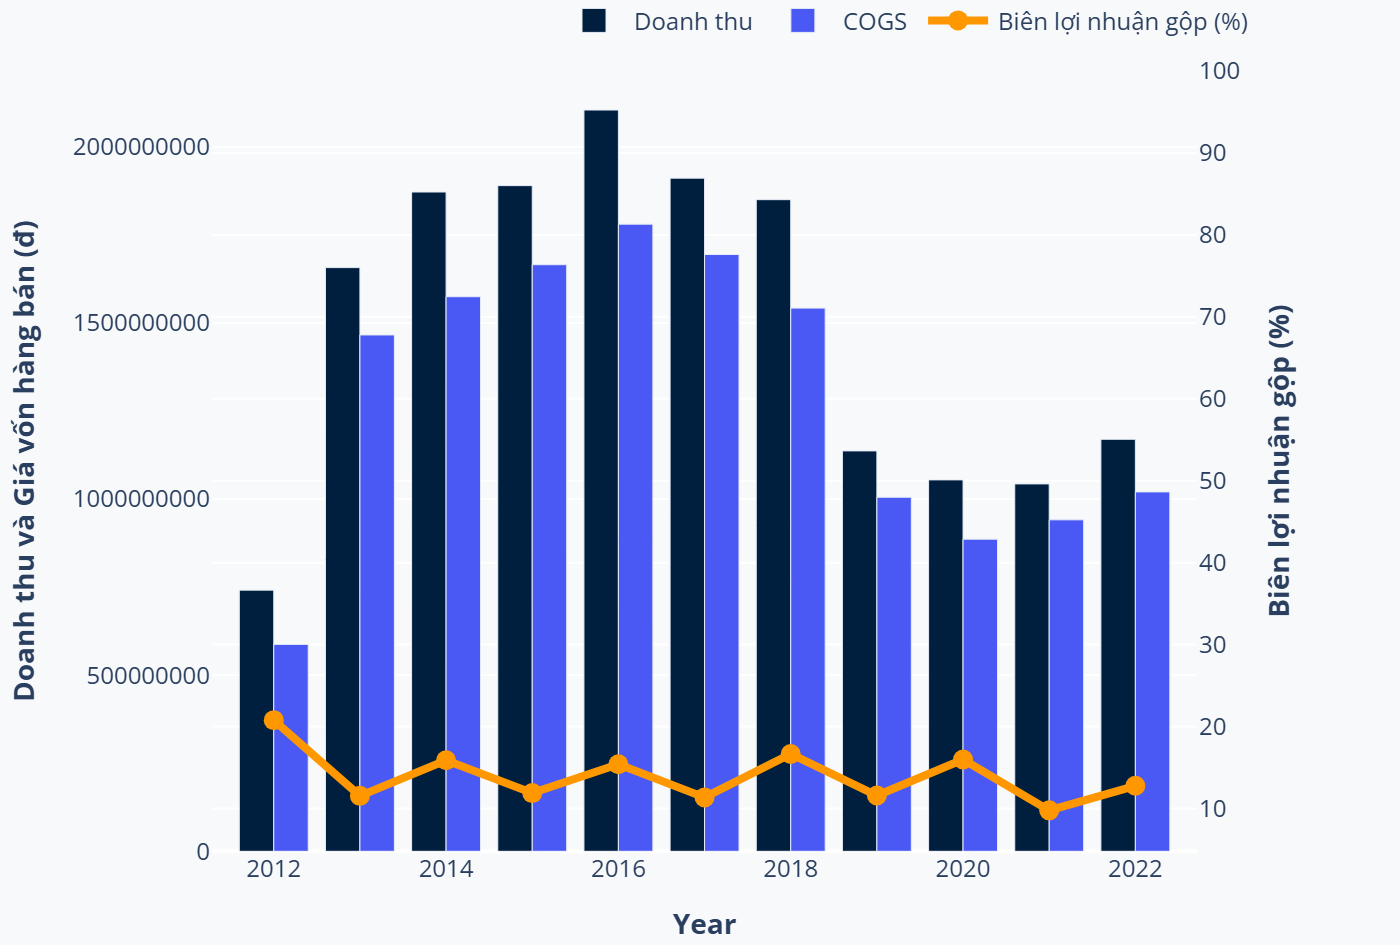
\includegraphics[width=0.8\textwidth]{figures/Hình 2.1.png}
    \caption{Hình 2.1}
    \label{fig:2.1}
\end{figure}

\begin{figure}[H]
    \centering
    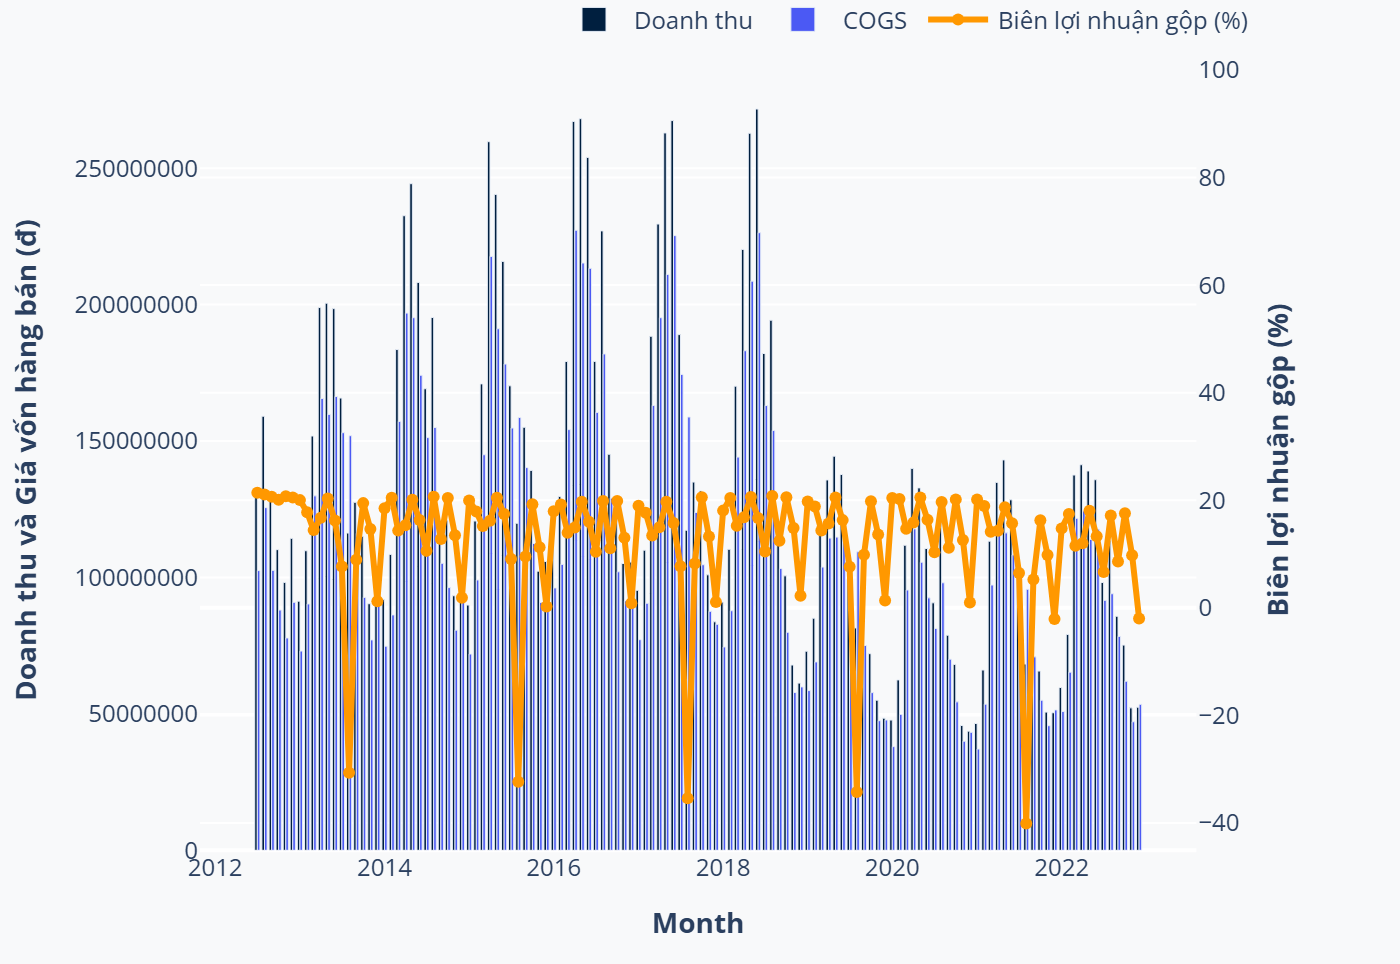
\includegraphics[width=0.8\textwidth]{figures/Hình 2.2.png}
    \caption{Hình 2.2}
    \label{fig:2.2}
\end{figure}

\begin{figure}[H]
    \centering
    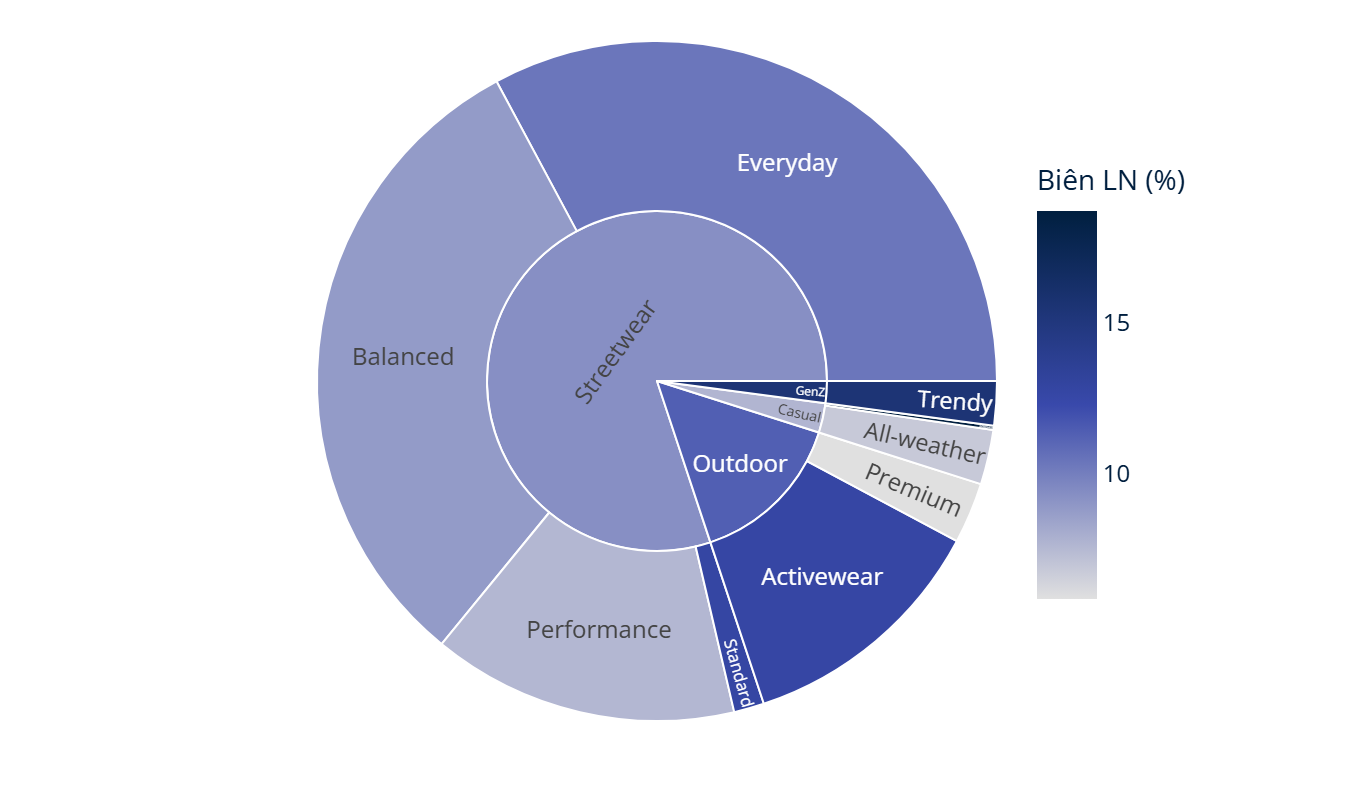
\includegraphics[width=0.8\textwidth]{figures/Hình 2.3.png}
    \caption{Hình 2.3}
    \label{fig:2.3}
\end{figure}

\begin{figure}[H]
    \centering
    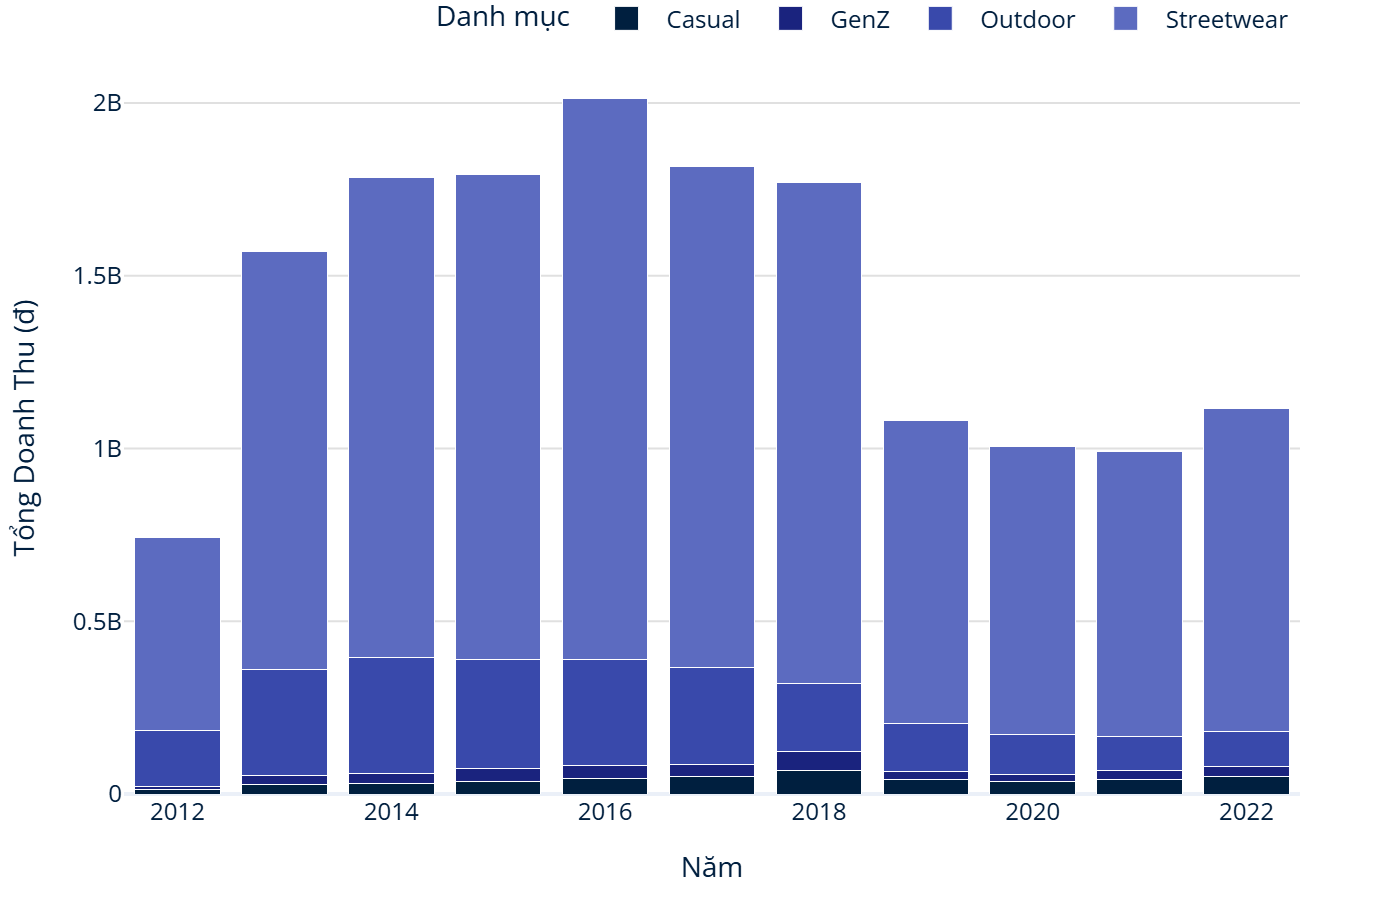
\includegraphics[width=0.8\textwidth]{figures/Hình 2.4.png}
    \caption{Hình 2.4}
    \label{fig:2.4}
\end{figure}

\begin{figure}[H]
    \centering
    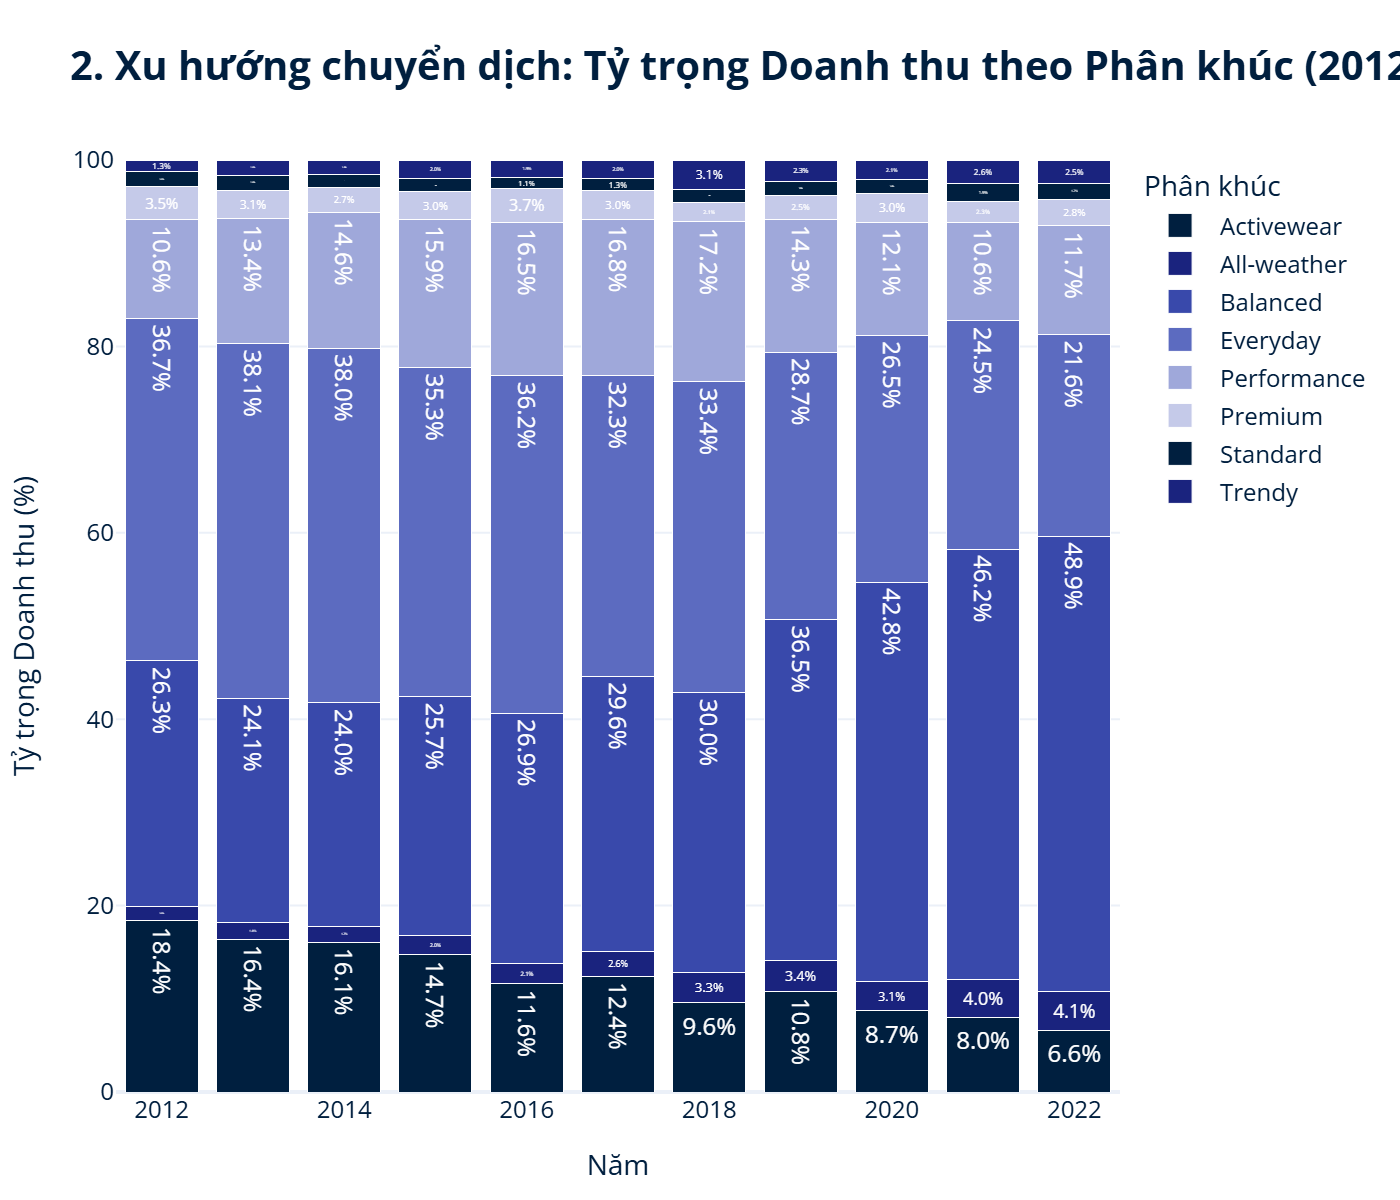
\includegraphics[width=0.8\textwidth]{figures/Hình 2.5.png}
    \caption{Hình 2.5}
    \label{fig:2.5}
\end{figure}

\begin{figure}[H]
    \centering
    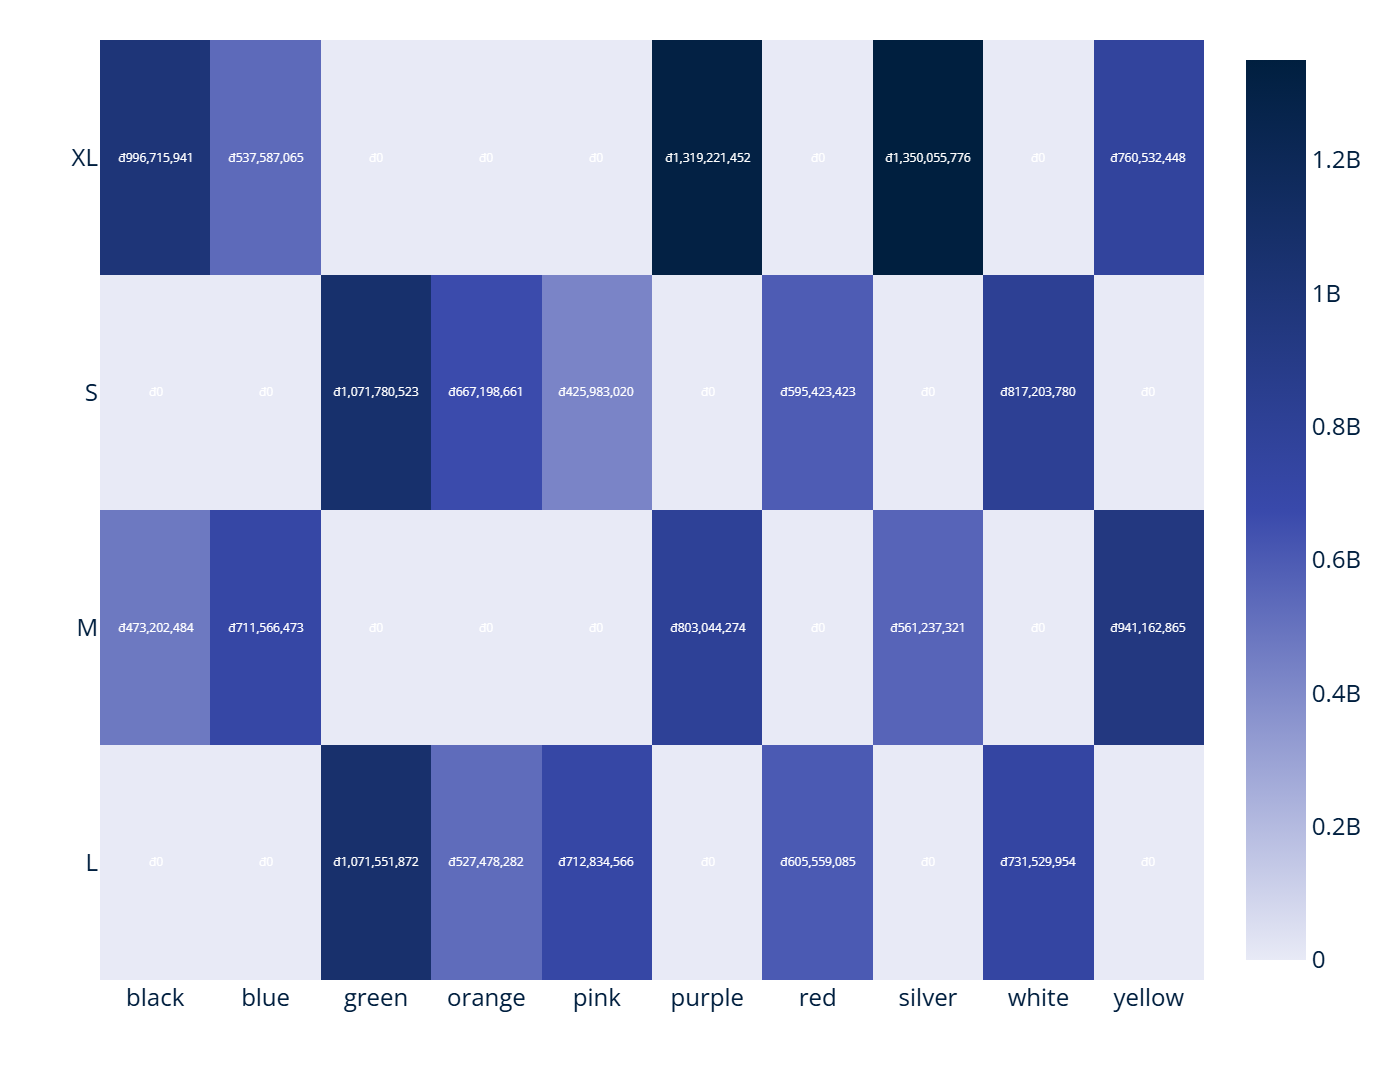
\includegraphics[width=0.8\textwidth]{figures/Hình 2.6.png}
    \caption{Hình 2.6}
    \label{fig:2.6}
\end{figure}

\begin{figure}[H]
    \centering
    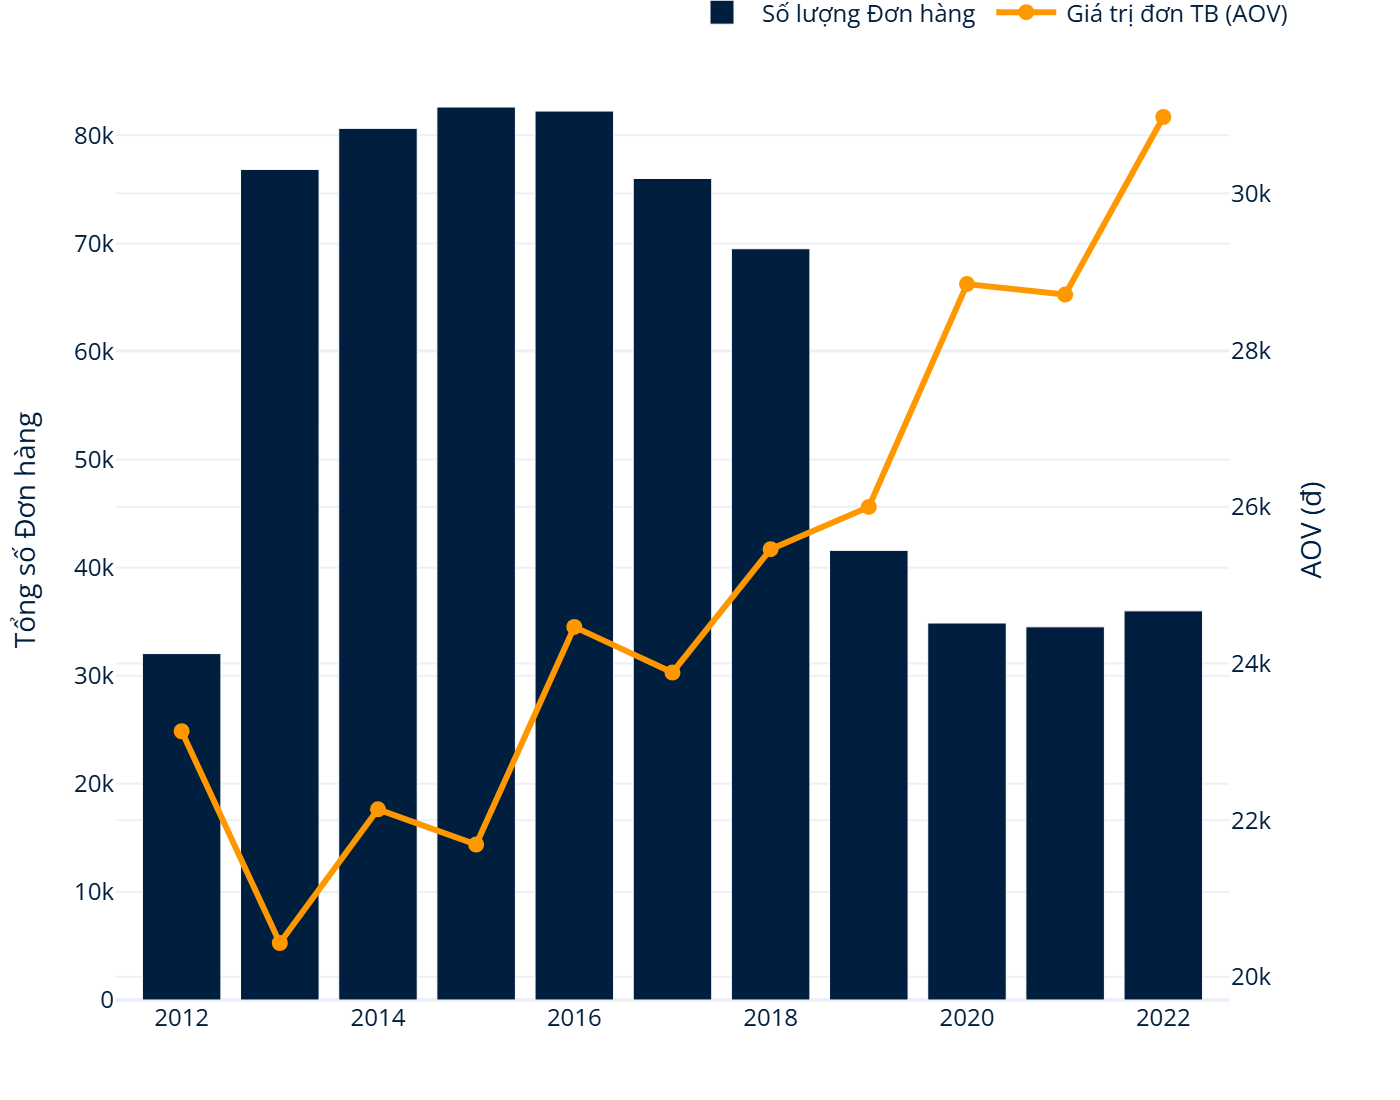
\includegraphics[width=0.8\textwidth]{figures/Hình 2.7a.png}
    \caption{Hình 2.7a}
    \label{fig:2.7a}
\end{figure}

\begin{figure}[H]
    \centering
    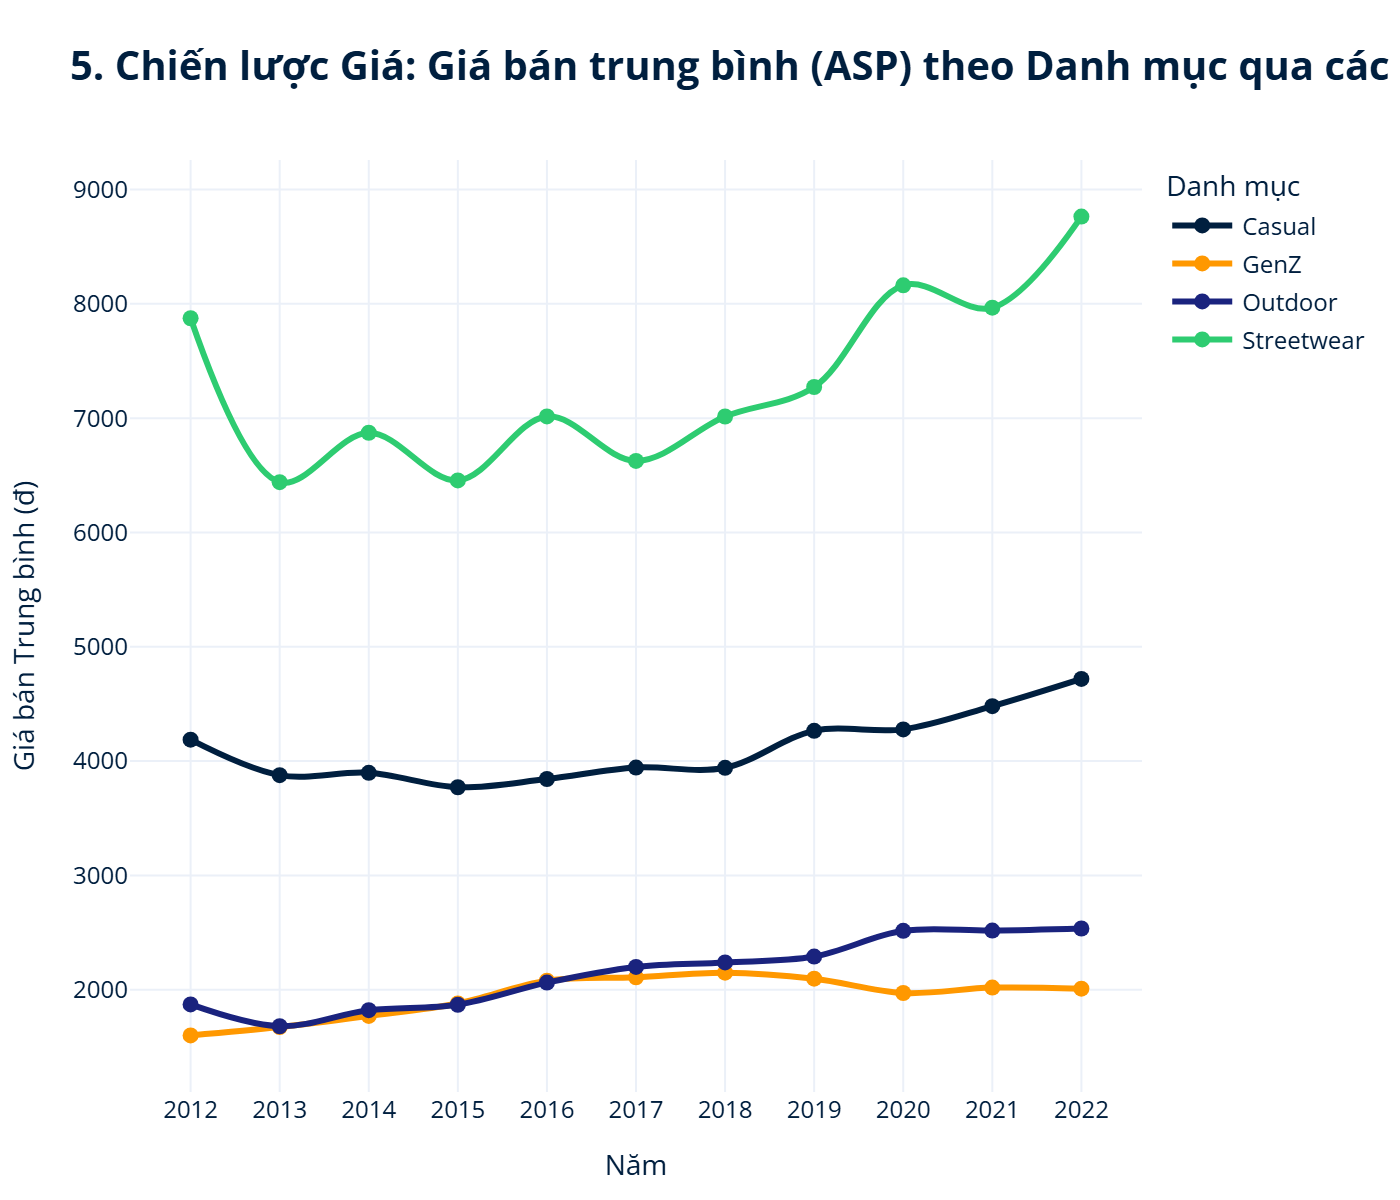
\includegraphics[width=0.8\textwidth]{figures/Hình 2.7b.png}
    \caption{Hình 2.7b}
    \label{fig:2.7b}
\end{figure}

\begin{figure}[H]
    \centering
    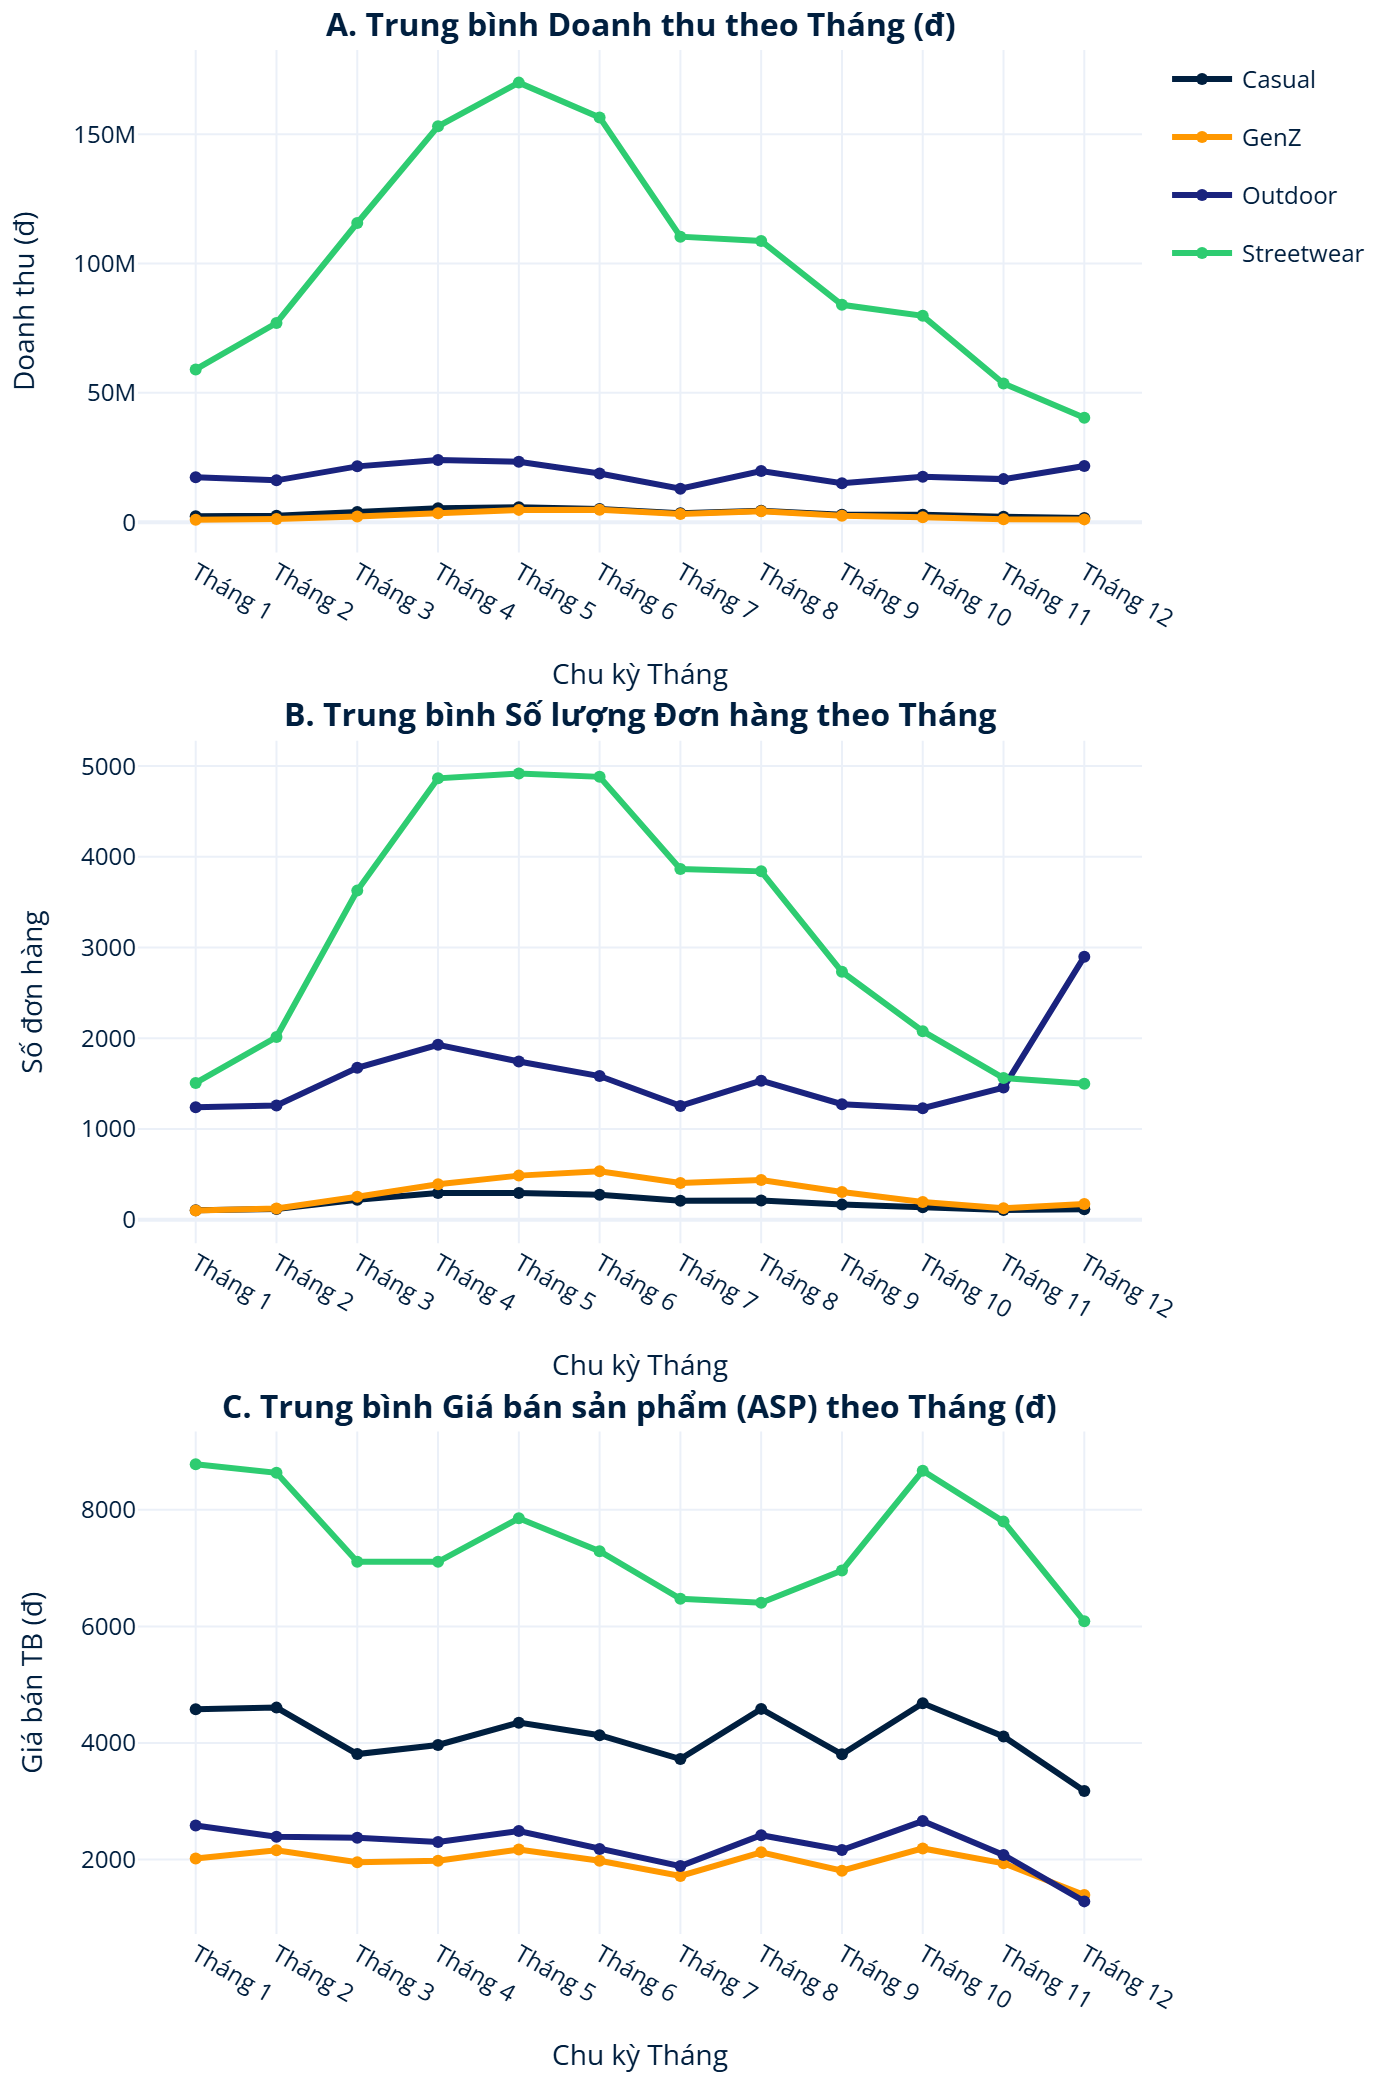
\includegraphics[width=0.8\textwidth]{figures/Hình 2.8.png}
    \caption{Hình 2.8}
    \label{fig:2.8}
\end{figure}

\begin{figure}[H]
    \centering
    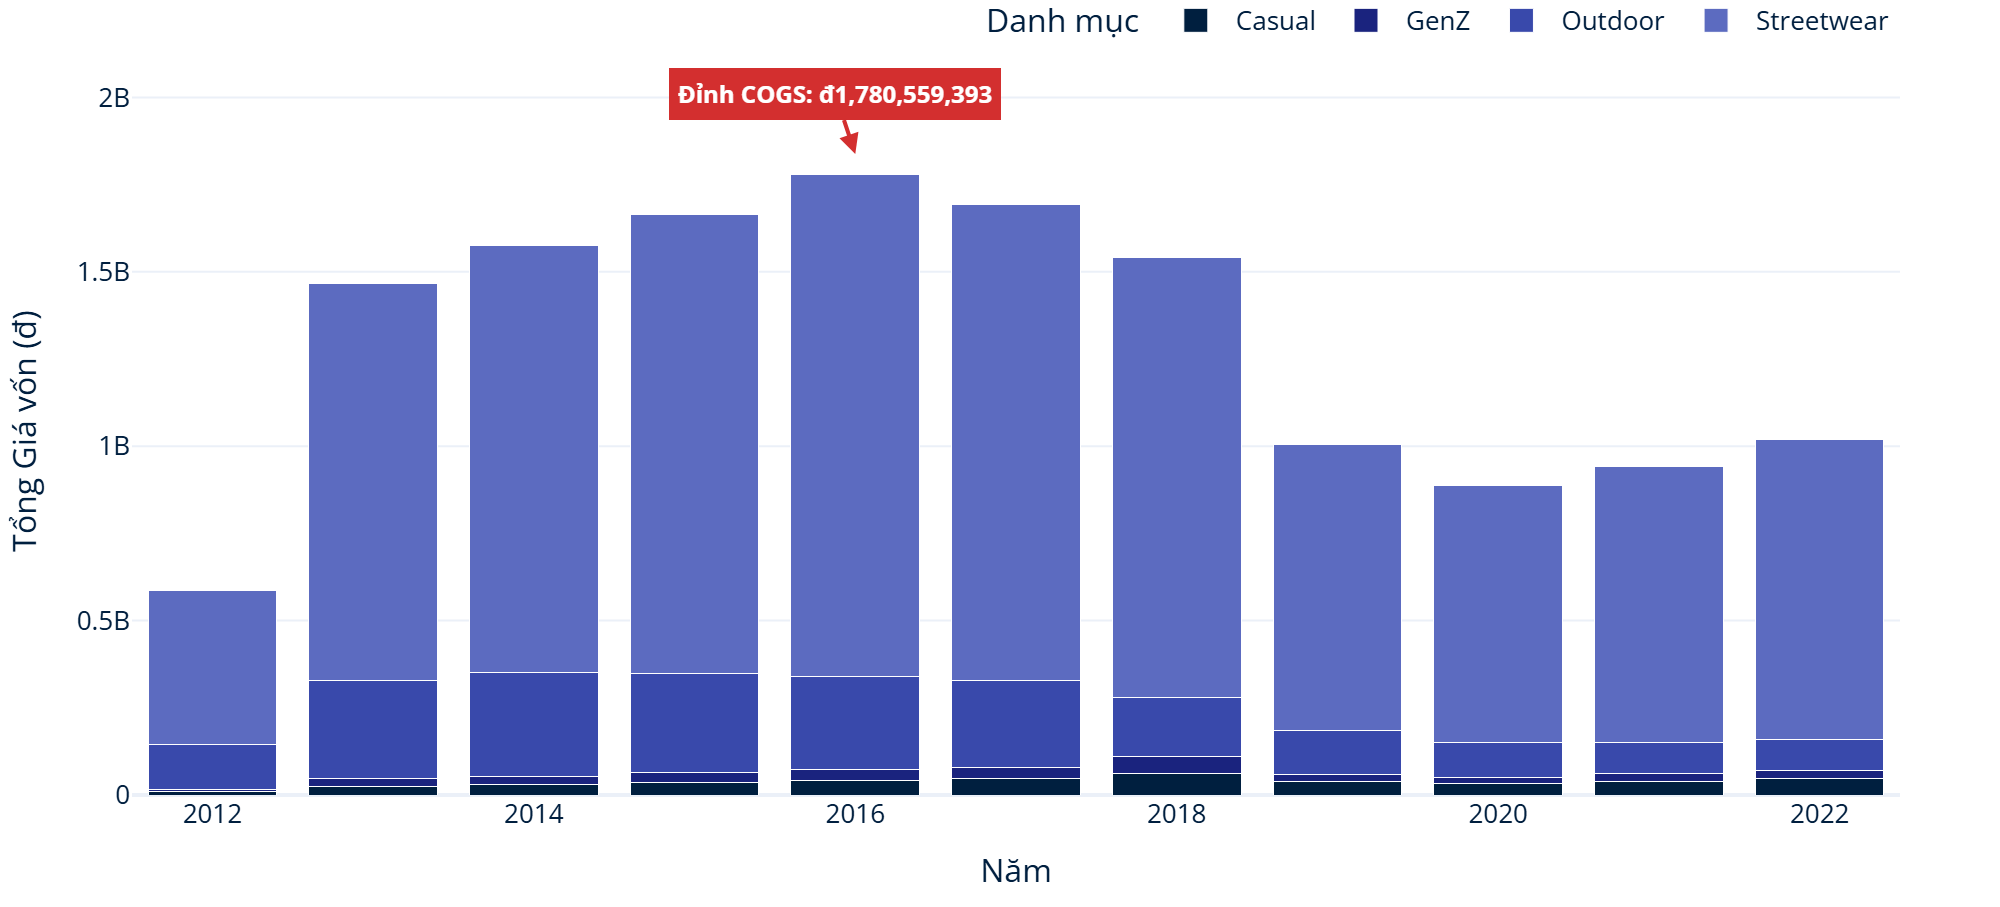
\includegraphics[width=0.8\textwidth]{figures/Hình 2.9.png}
    \caption{Hình 2.9}
    \label{fig:2.9}
\end{figure}

\begin{figure}[H]
    \centering
    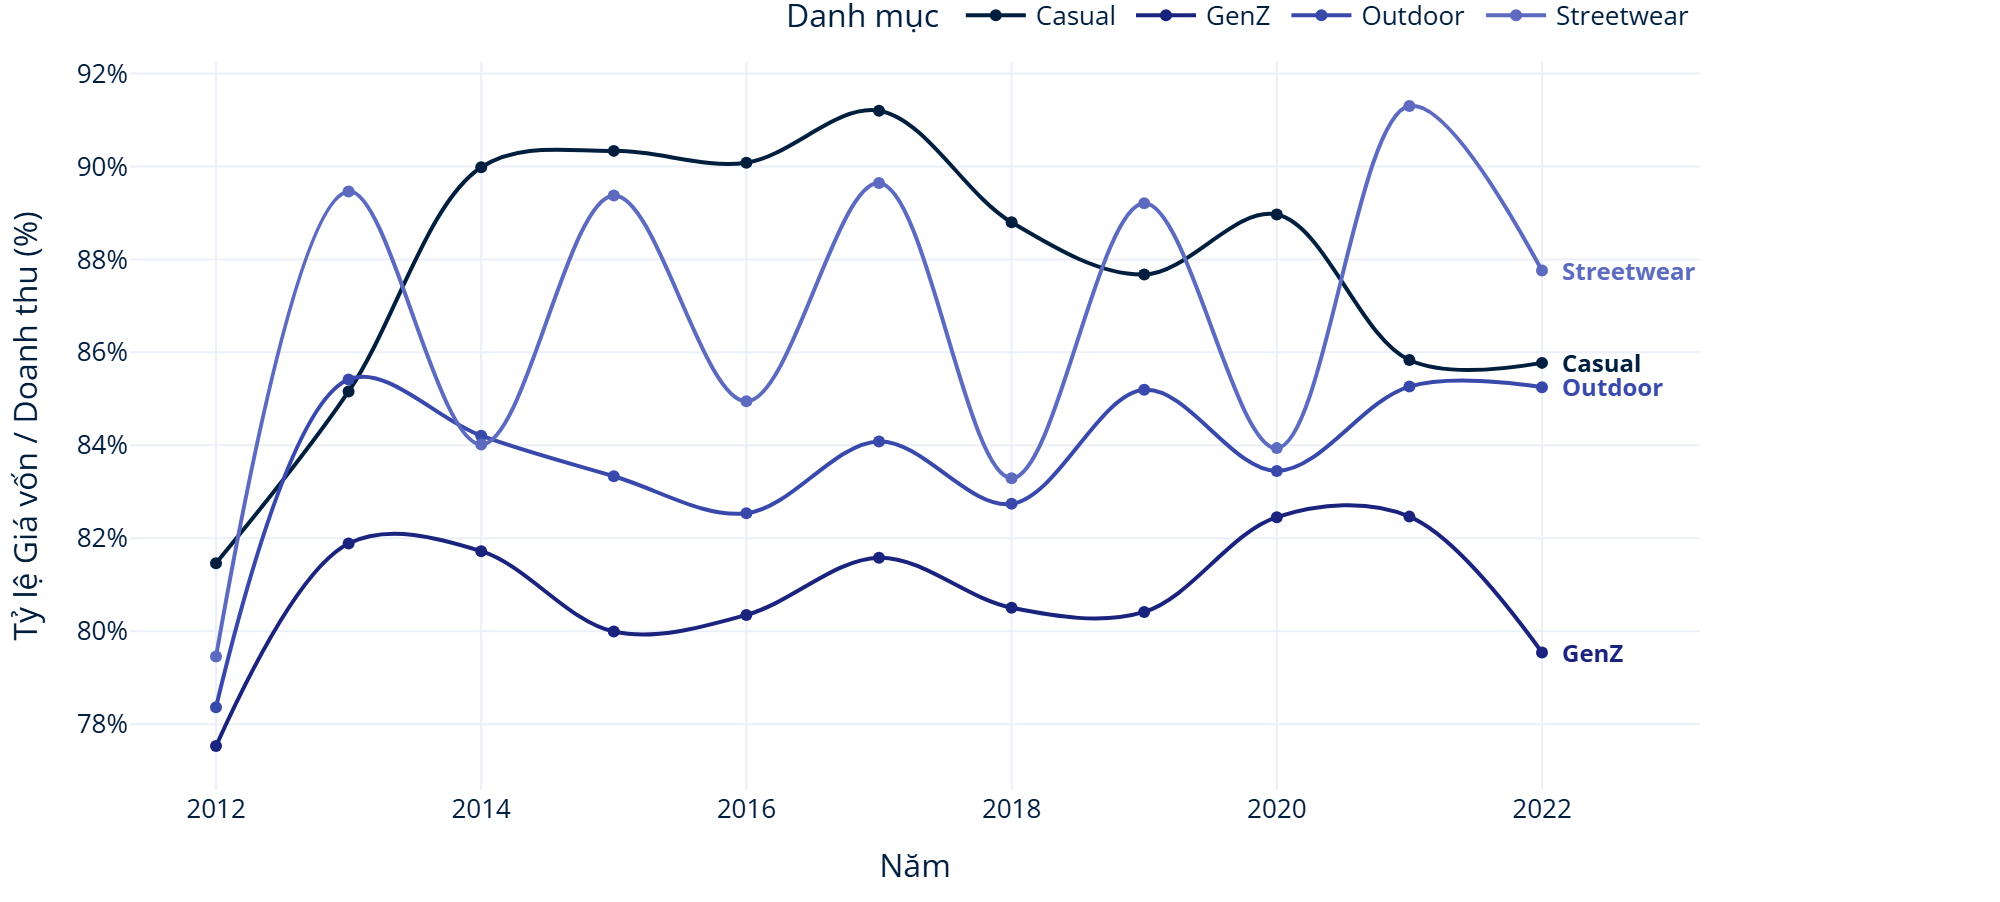
\includegraphics[width=0.8\textwidth]{figures/Hình 2.10.png}
    \caption{Hình 2.10}
    \label{fig:2.10}
\end{figure}

\begin{figure}[H]
    \centering
    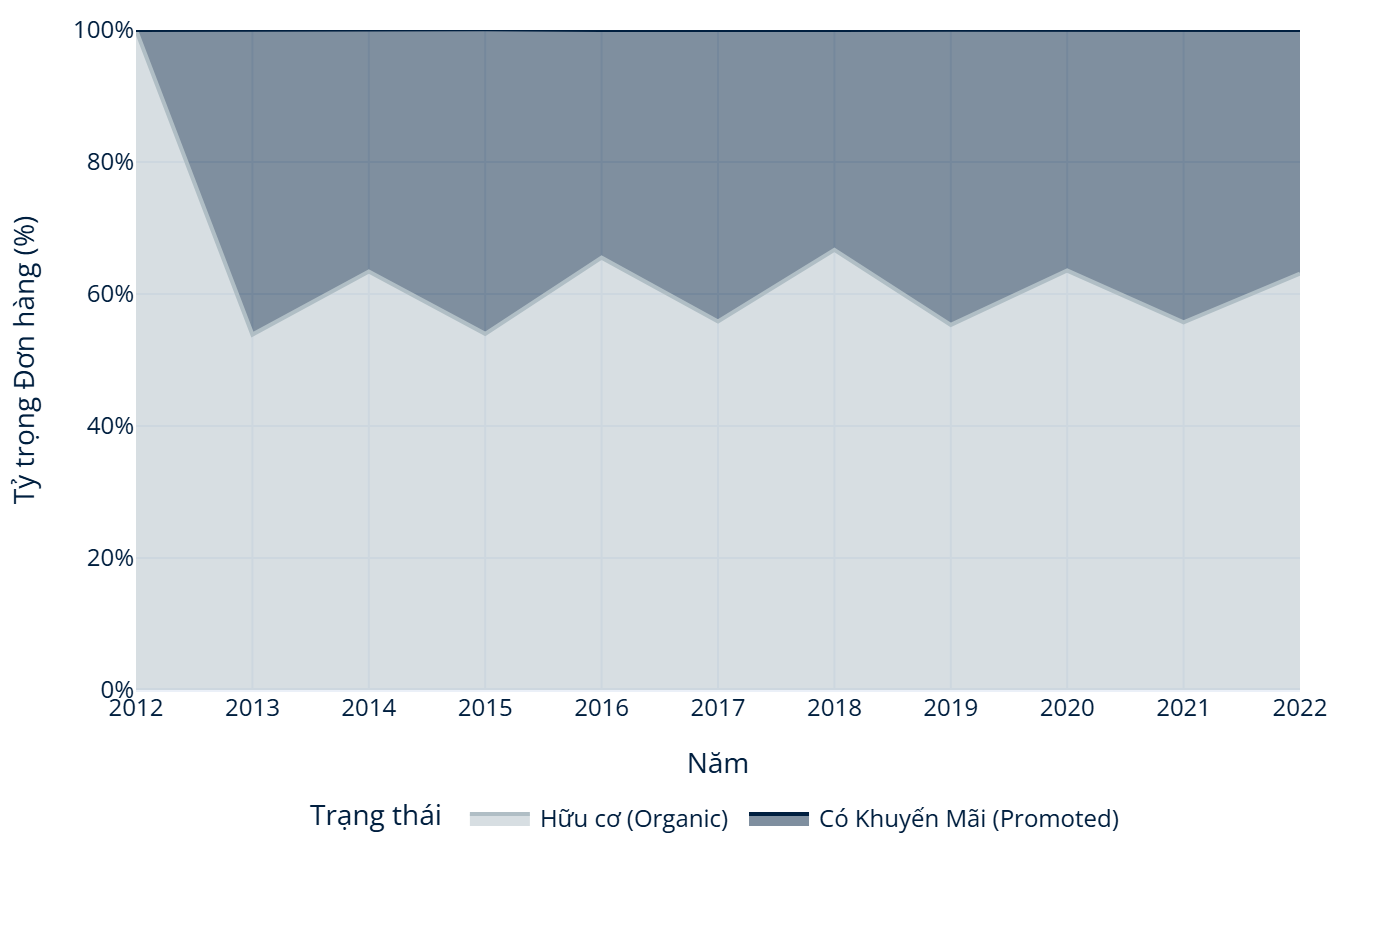
\includegraphics[width=0.8\textwidth]{figures/Hình 2.11.png}
    \caption{Hình 2.11}
    \label{fig:2.11}
\end{figure}

\begin{figure}[H]
    \centering
    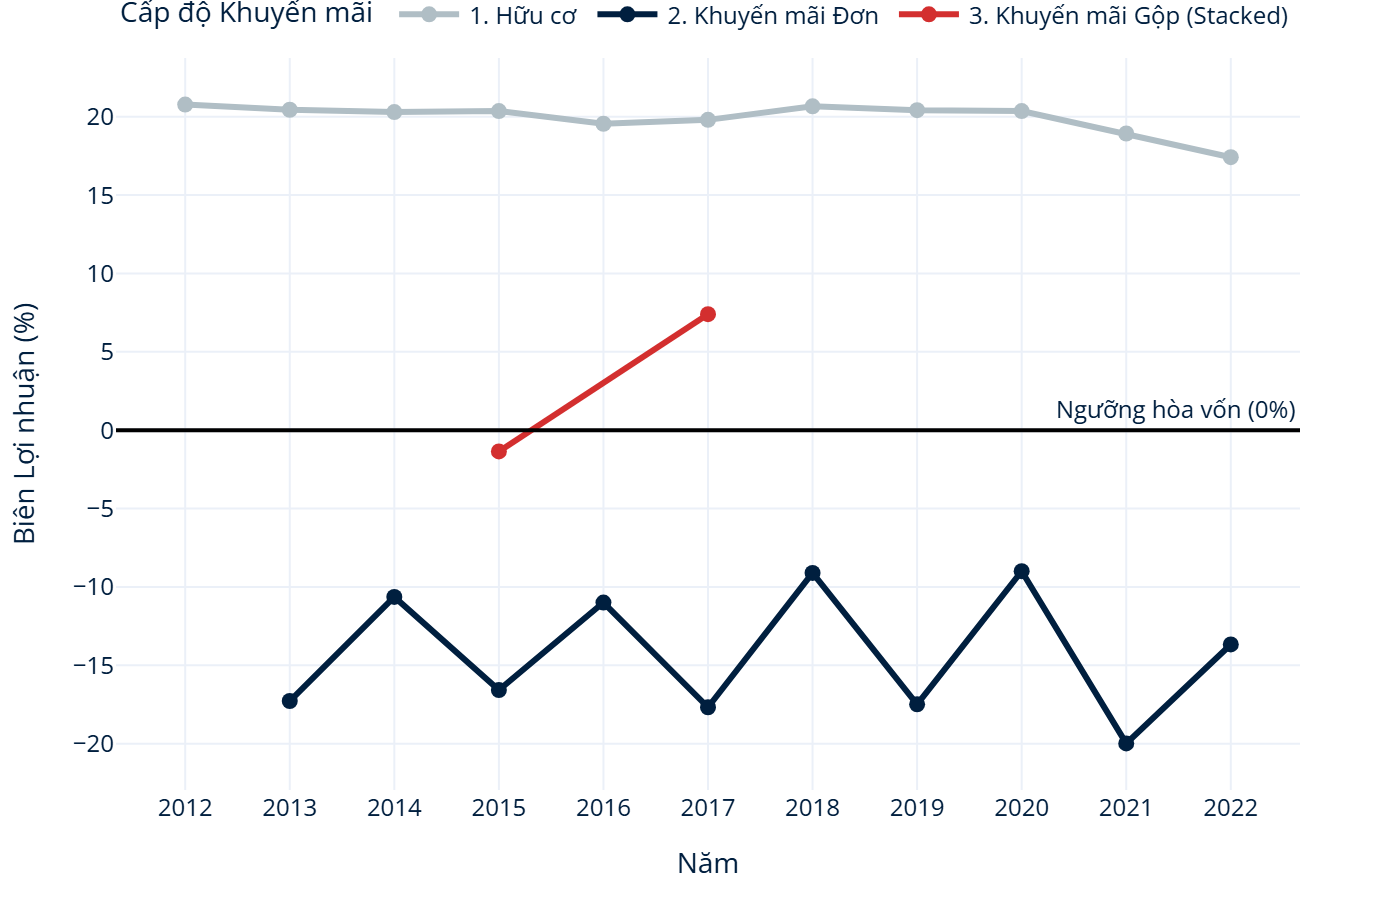
\includegraphics[width=0.8\textwidth]{figures/Hình 2.12.png}
    \caption{Hình 2.12}
    \label{fig:2.12}
\end{figure}

\begin{figure}[H]
    \centering
    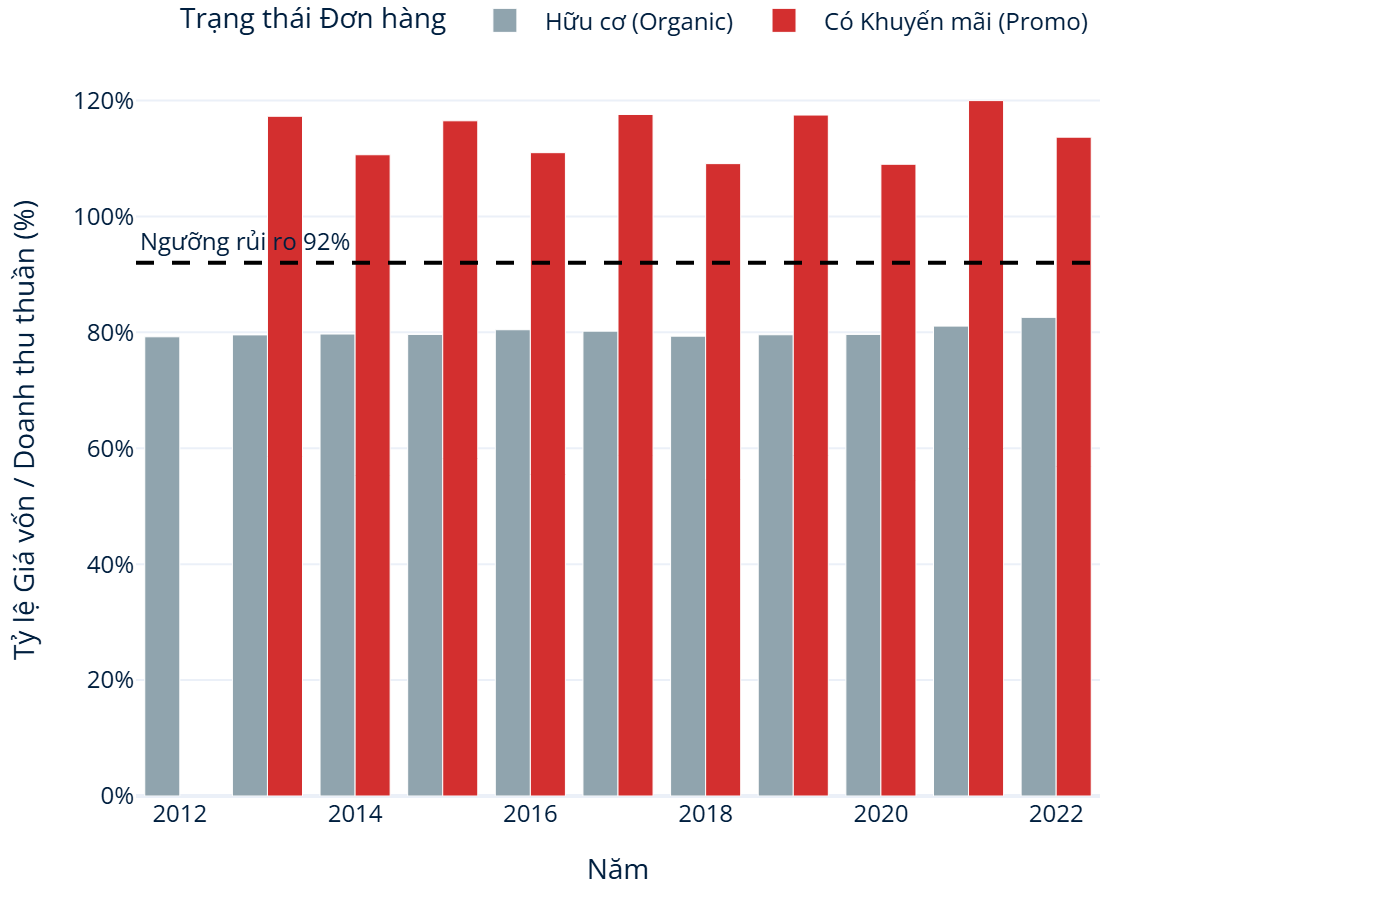
\includegraphics[width=0.8\textwidth]{figures/Hình 2.13a.png}
    \caption{Hình 2.13a}
    \label{fig:2.13a}
\end{figure}

\begin{figure}[H]
    \centering
    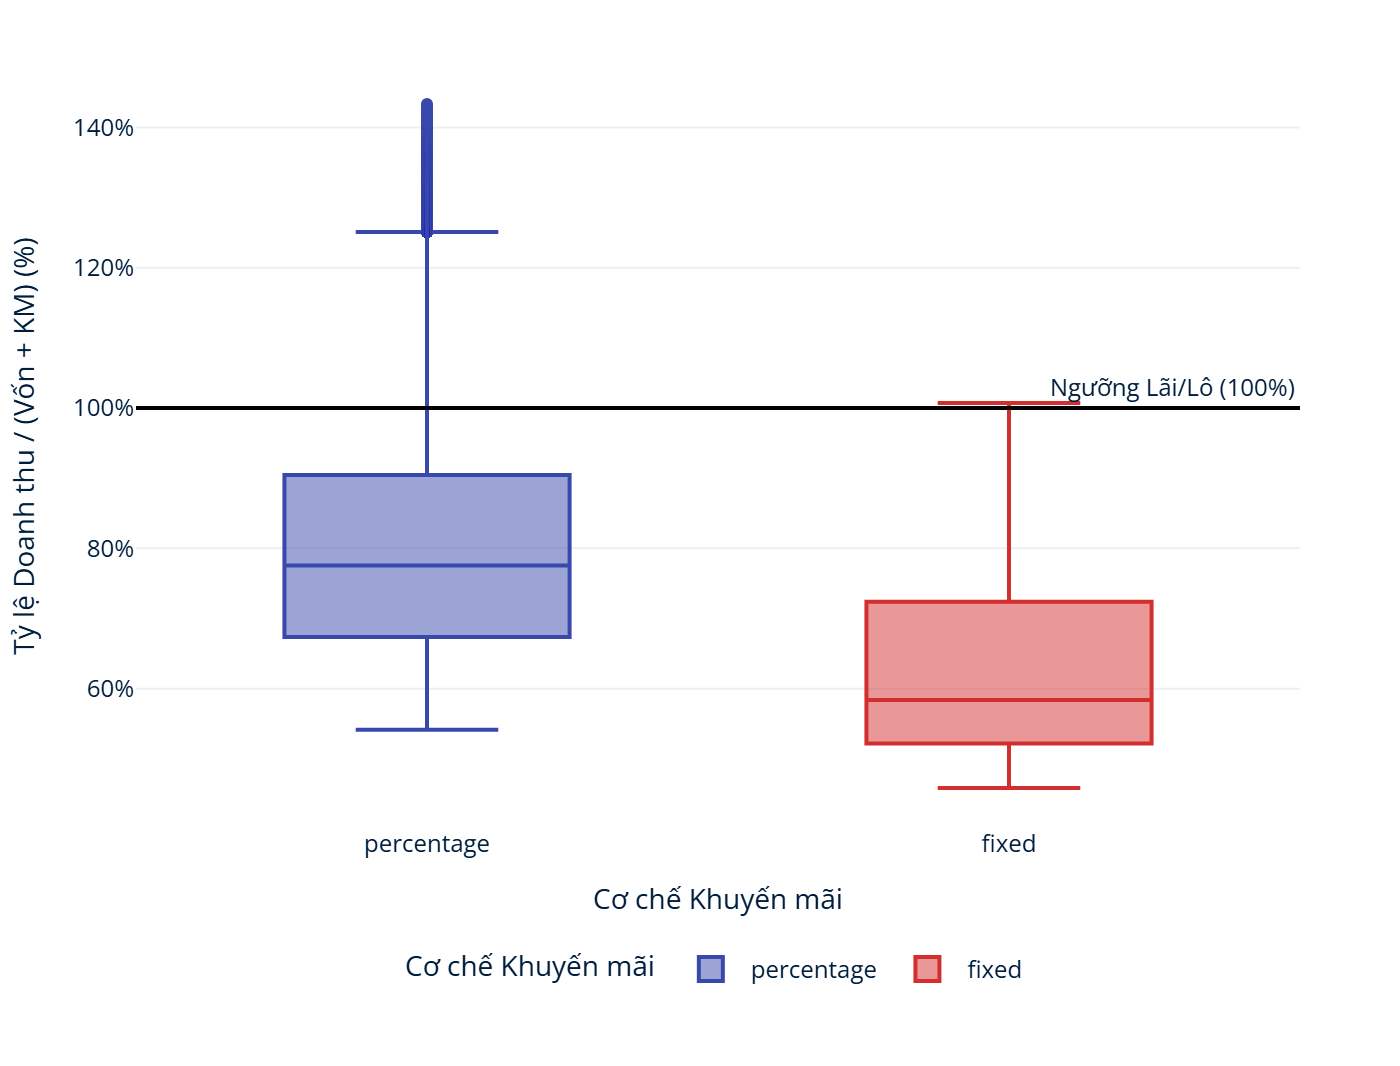
\includegraphics[width=0.8\textwidth]{figures/Hình 2.13b.png}
    \caption{Hình 2.13b}
    \label{fig:2.13b}
\end{figure}

\begin{figure}[H]
    \centering
    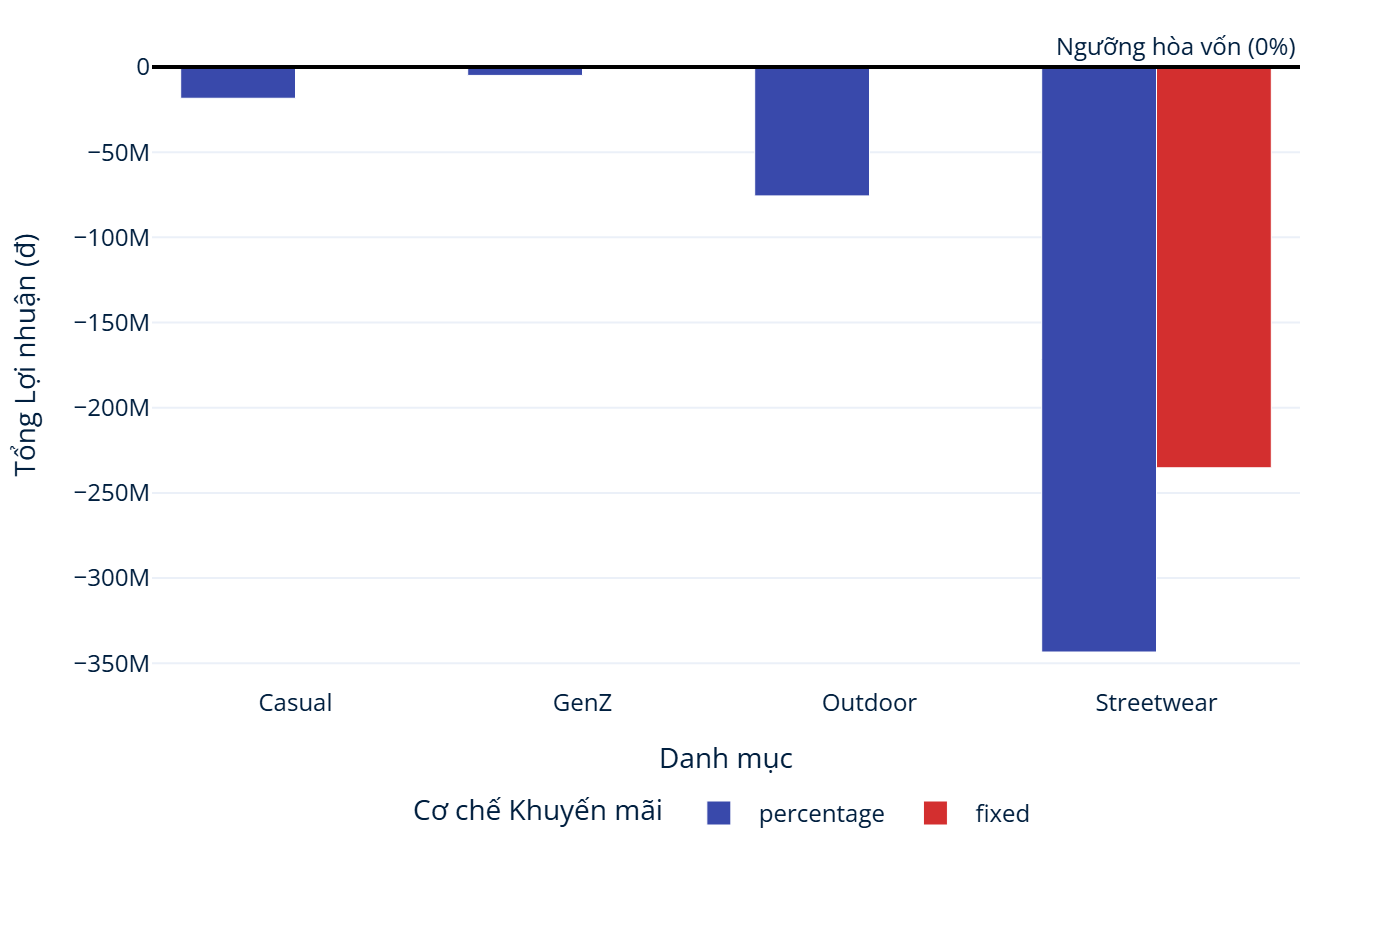
\includegraphics[width=0.8\textwidth]{figures/Hình 2.13c.png}
    \caption{Hình 2.13c}
    \label{fig:2.13c}
\end{figure}

\begin{figure}[H]
    \centering
    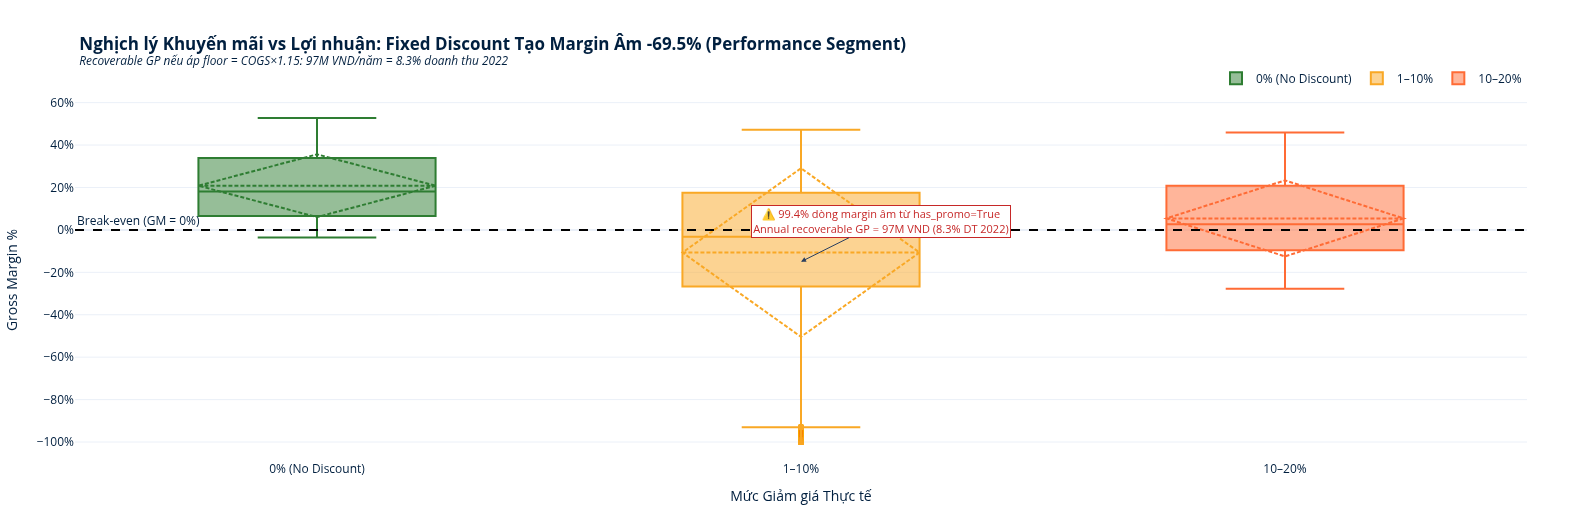
\includegraphics[width=0.8\textwidth]{figures/Hình 2.13d.png}
    \caption{Hình 2.13d}
    \label{fig:2.13d}
\end{figure}

\begin{figure}[H]
    \centering
    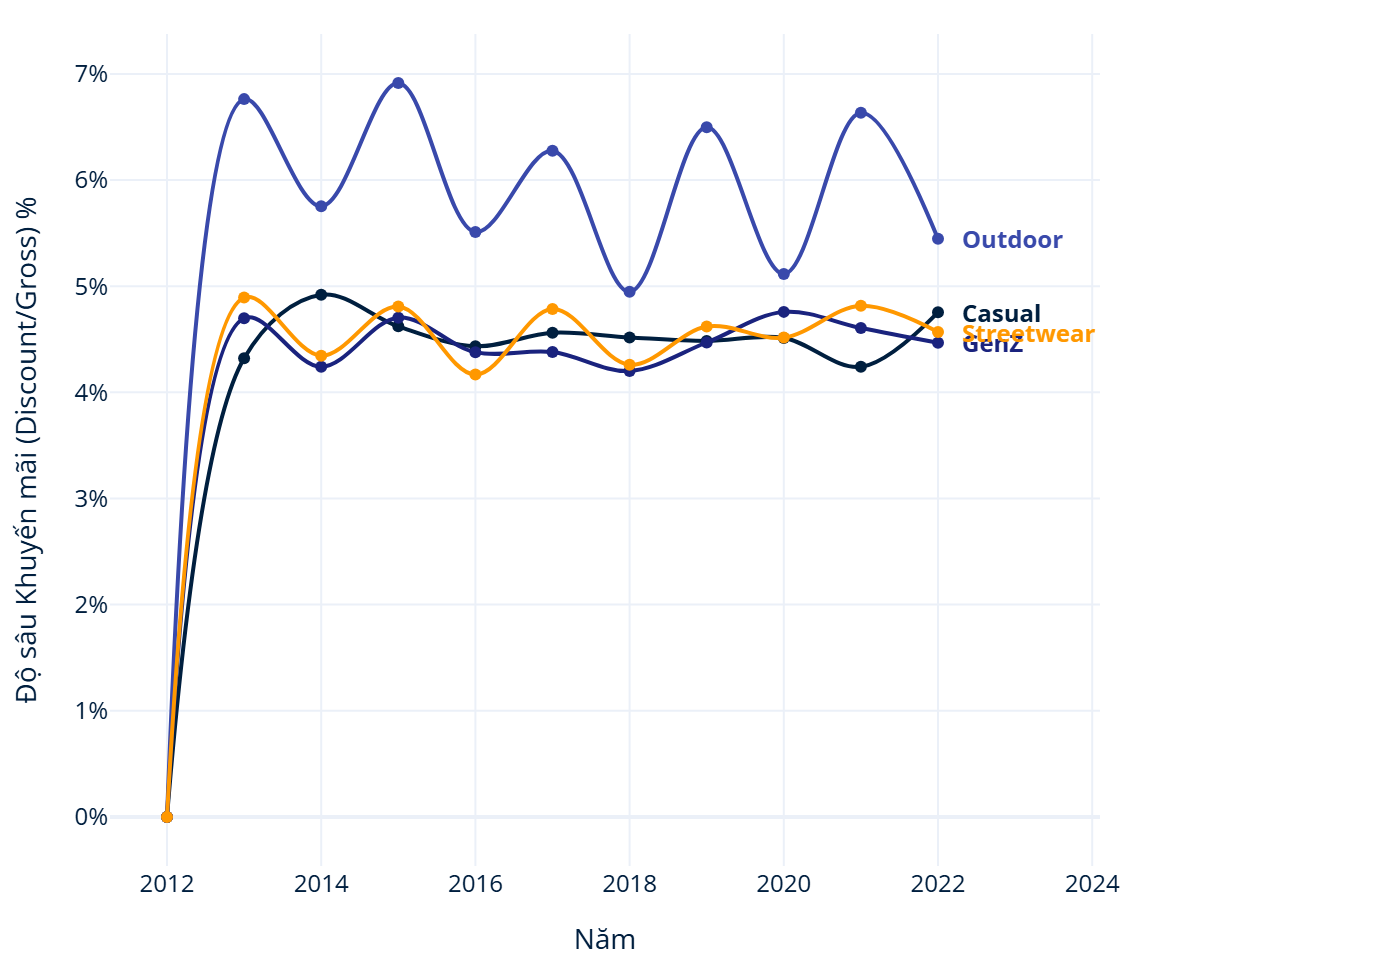
\includegraphics[width=0.8\textwidth]{figures/Hình 2.14.png}
    \caption{Hình 2.14}
    \label{fig:2.14}
\end{figure}

\begin{figure}[H]
    \centering
    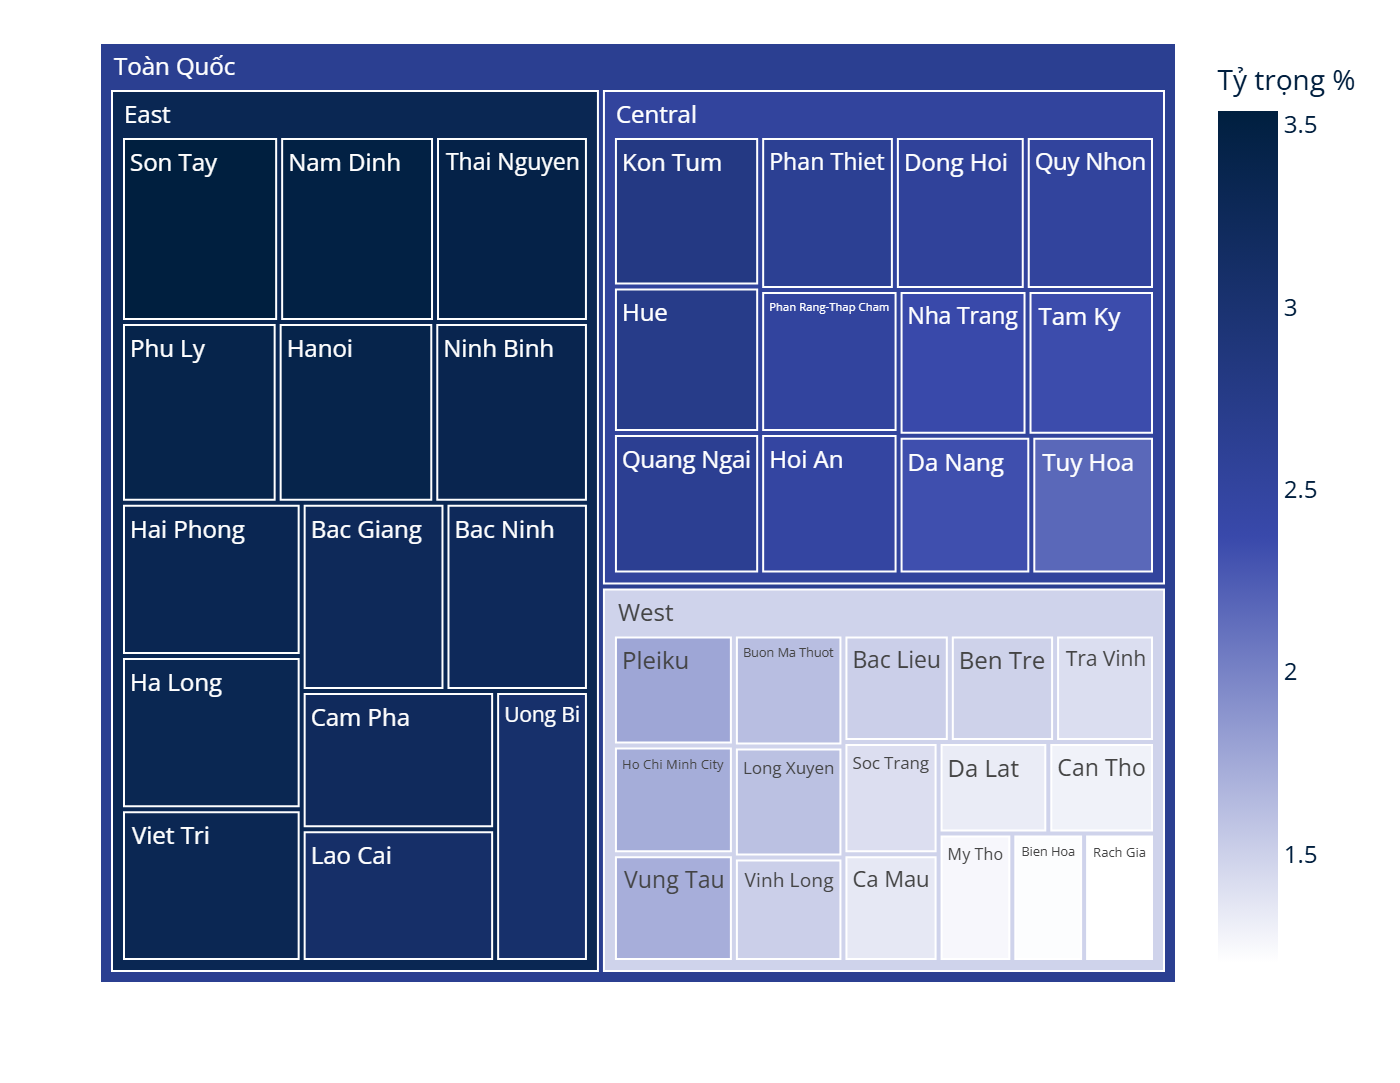
\includegraphics[width=0.8\textwidth]{figures/Hình 2.15.png}
    \caption{Hình 2.15}
    \label{fig:2.15}
\end{figure}

\begin{figure}[H]
    \centering
    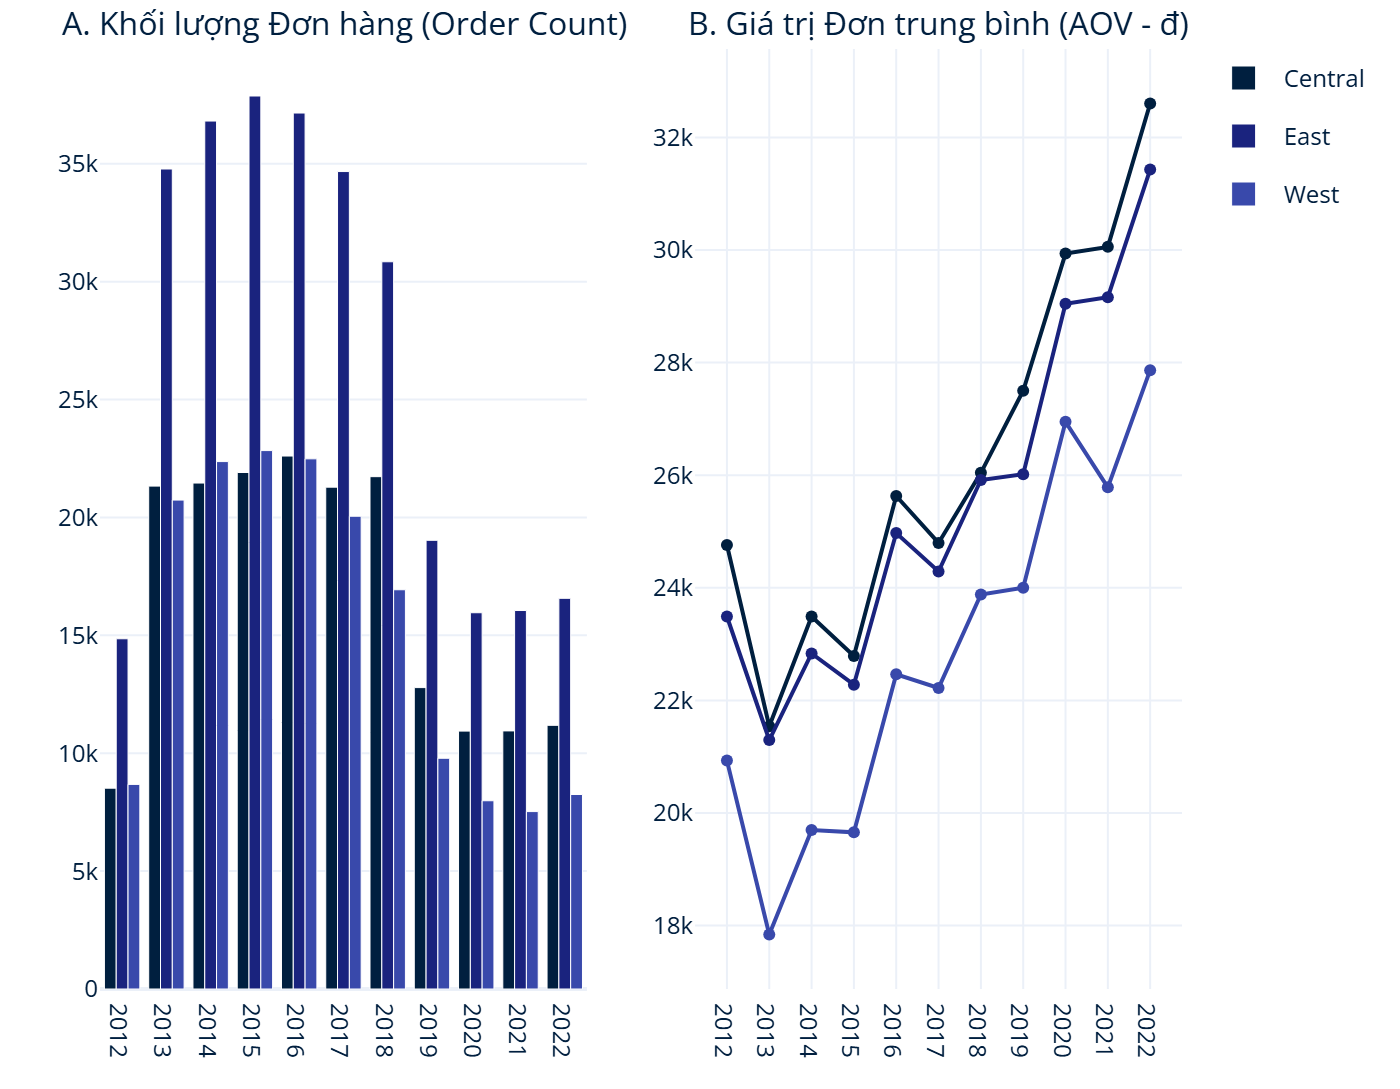
\includegraphics[width=0.8\textwidth]{figures/Hình 2.16.png}
    \caption{Hình 2.16}
    \label{fig:2.16}
\end{figure}

\begin{figure}[H]
    \centering
    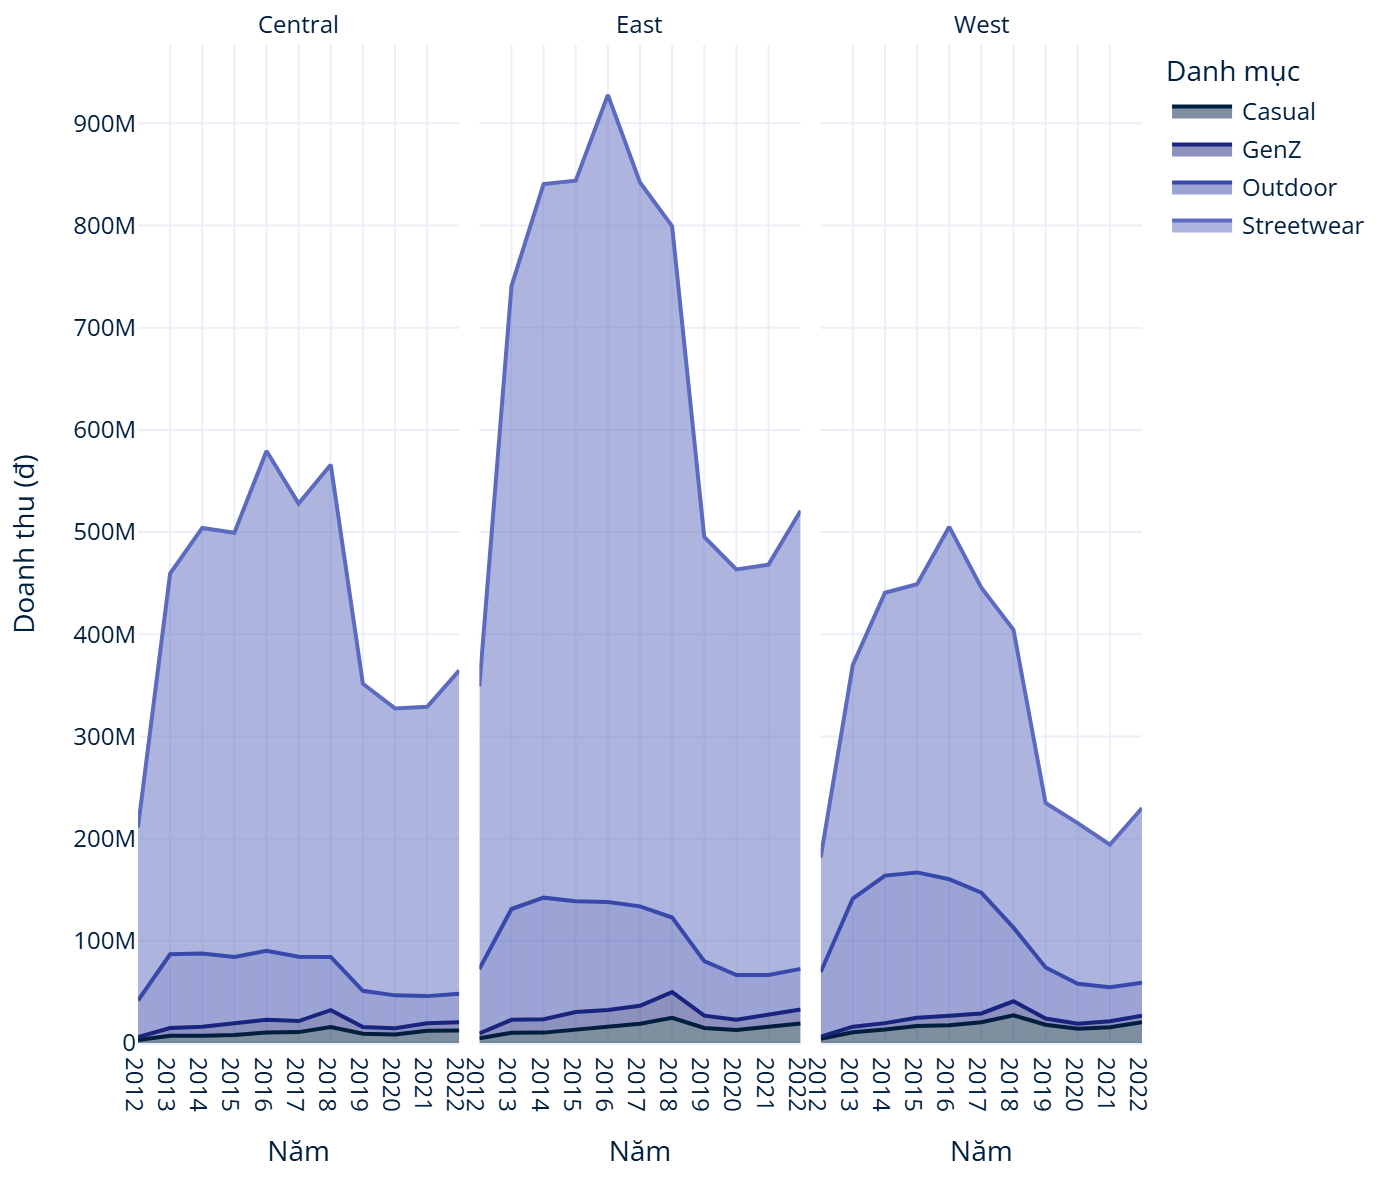
\includegraphics[width=0.8\textwidth]{figures/Hình 2.17.png}
    \caption{Hình 2.17}
    \label{fig:2.17}
\end{figure}

\begin{figure}[H]
    \centering
    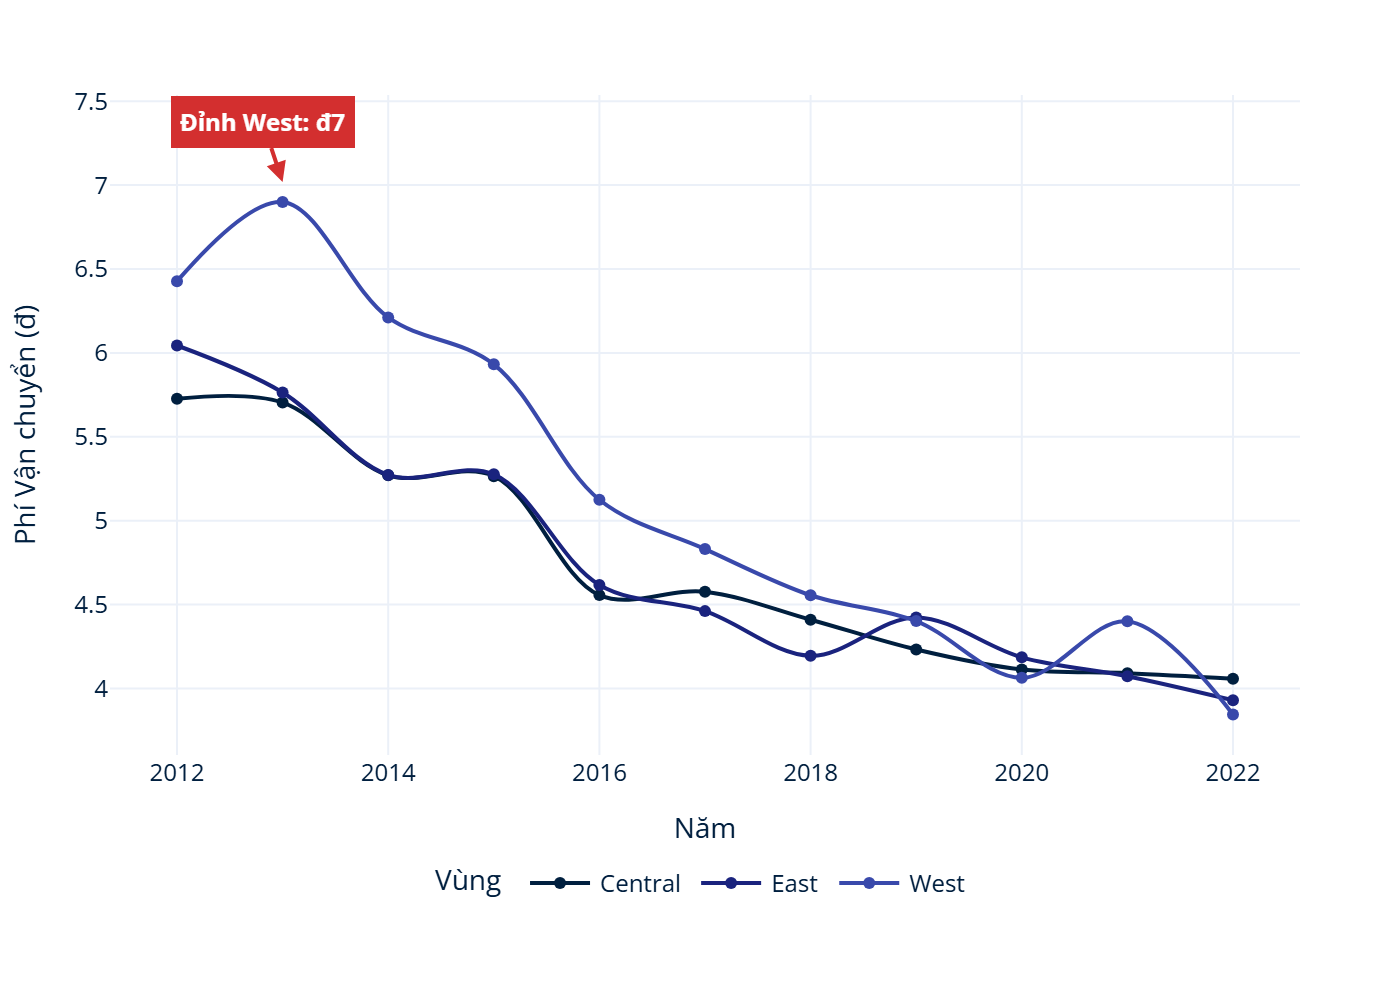
\includegraphics[width=0.8\textwidth]{figures/Hình 2.18.png}
    \caption{Hình 2.18}
    \label{fig:2.18}
\end{figure}

\begin{figure}[H]
    \centering
    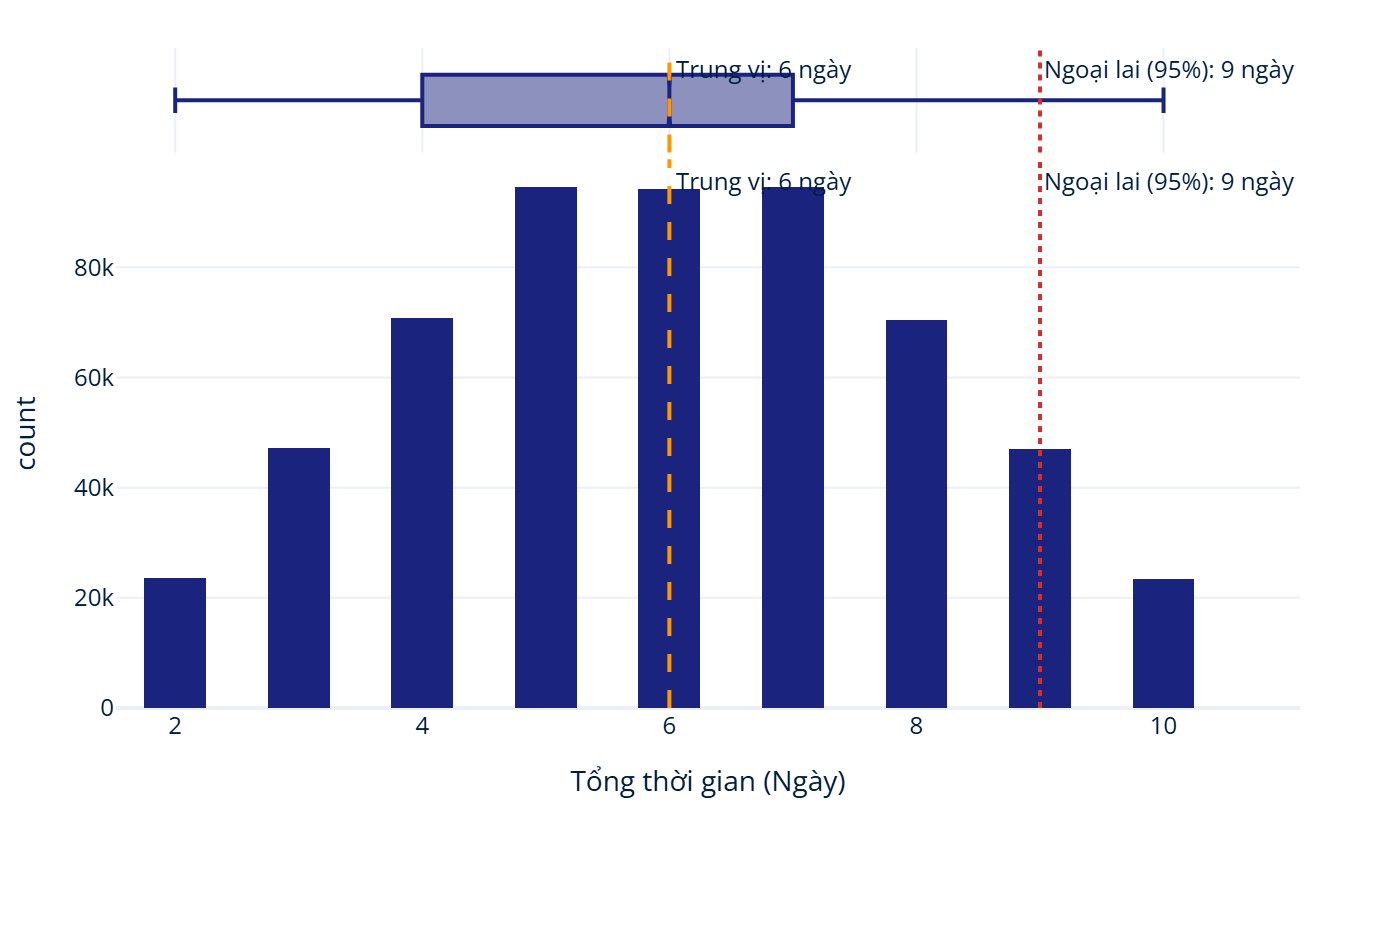
\includegraphics[width=0.8\textwidth]{figures/Hình 2.19.png}
    \caption{Hình 2.19}
    \label{fig:2.19}
\end{figure}

\begin{figure}[H]
    \centering
    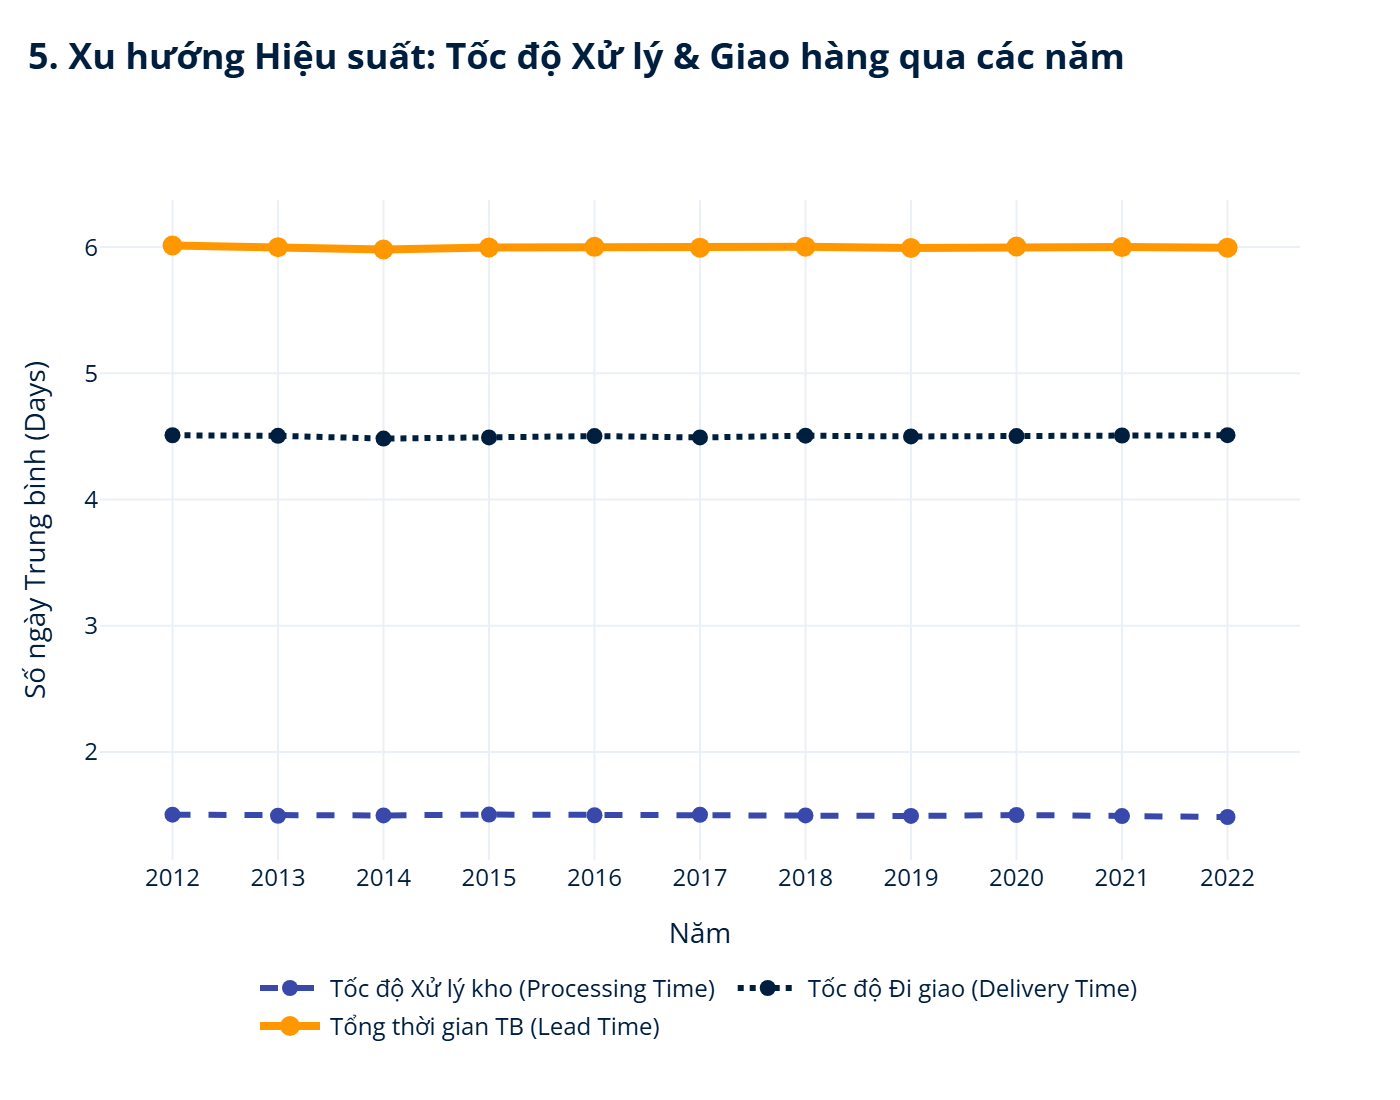
\includegraphics[width=0.8\textwidth]{figures/Hình 2.20.png}
    \caption{Hình 2.20}
    \label{fig:2.20}
\end{figure}

\begin{figure}[H]
    \centering
    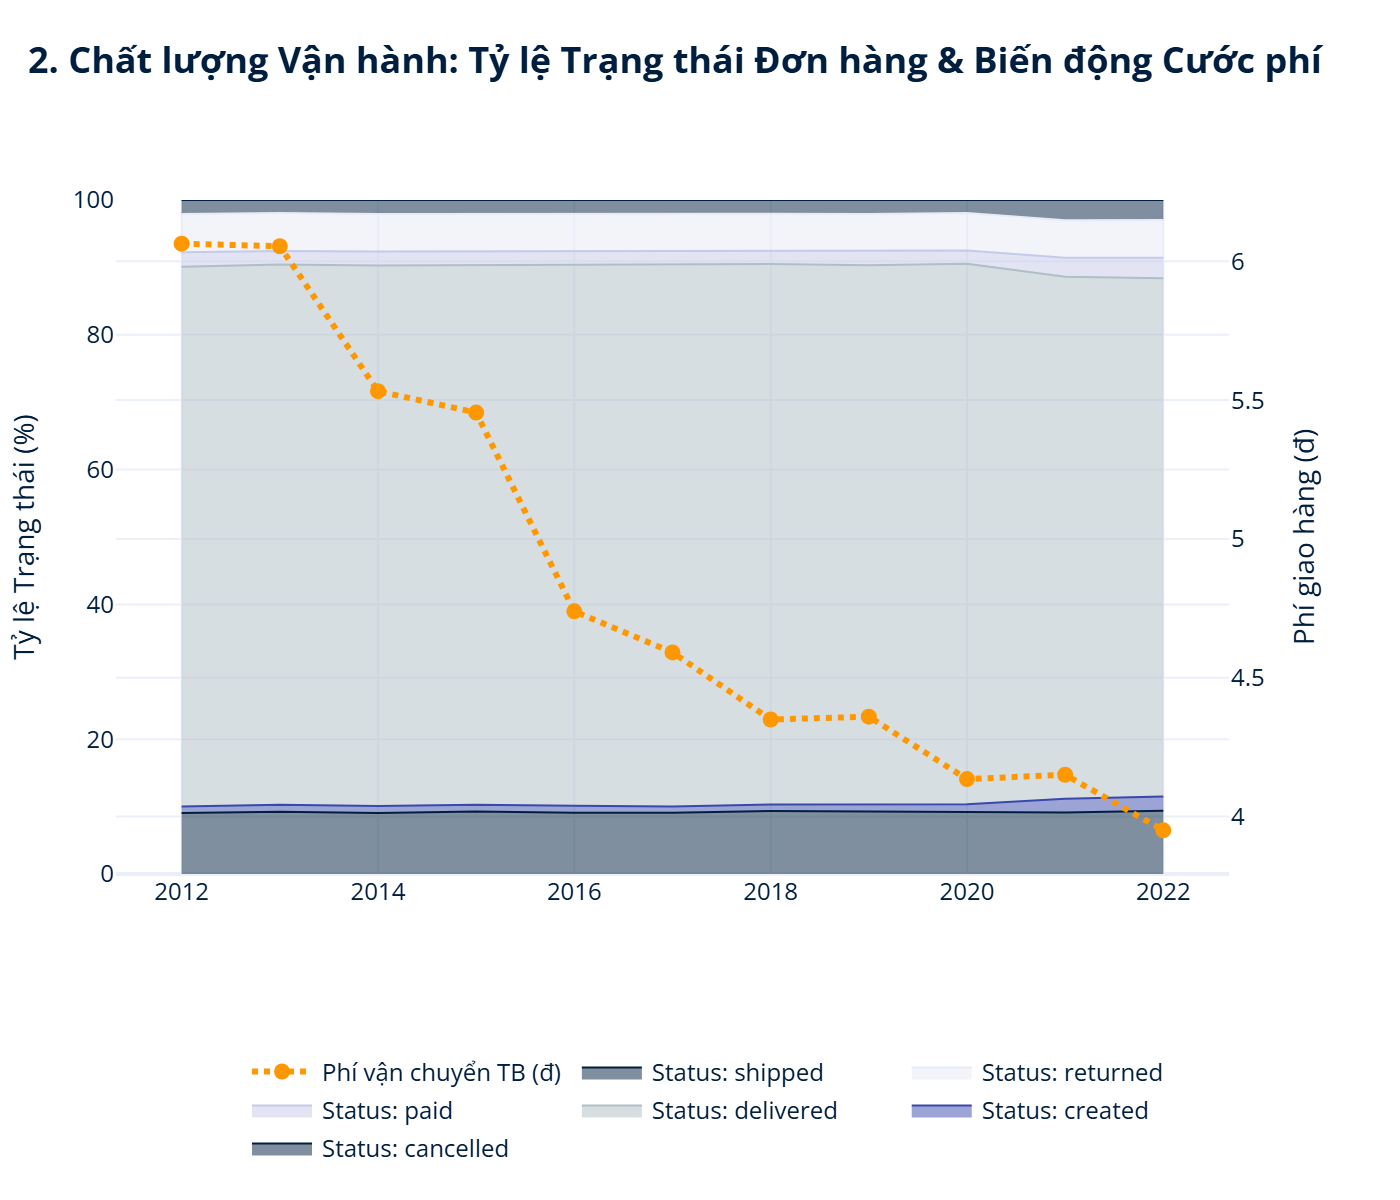
\includegraphics[width=0.8\textwidth]{figures/Hình 2.21.png}
    \caption{Hình 2.21}
    \label{fig:2.21}
\end{figure}

\begin{figure}[H]
    \centering
    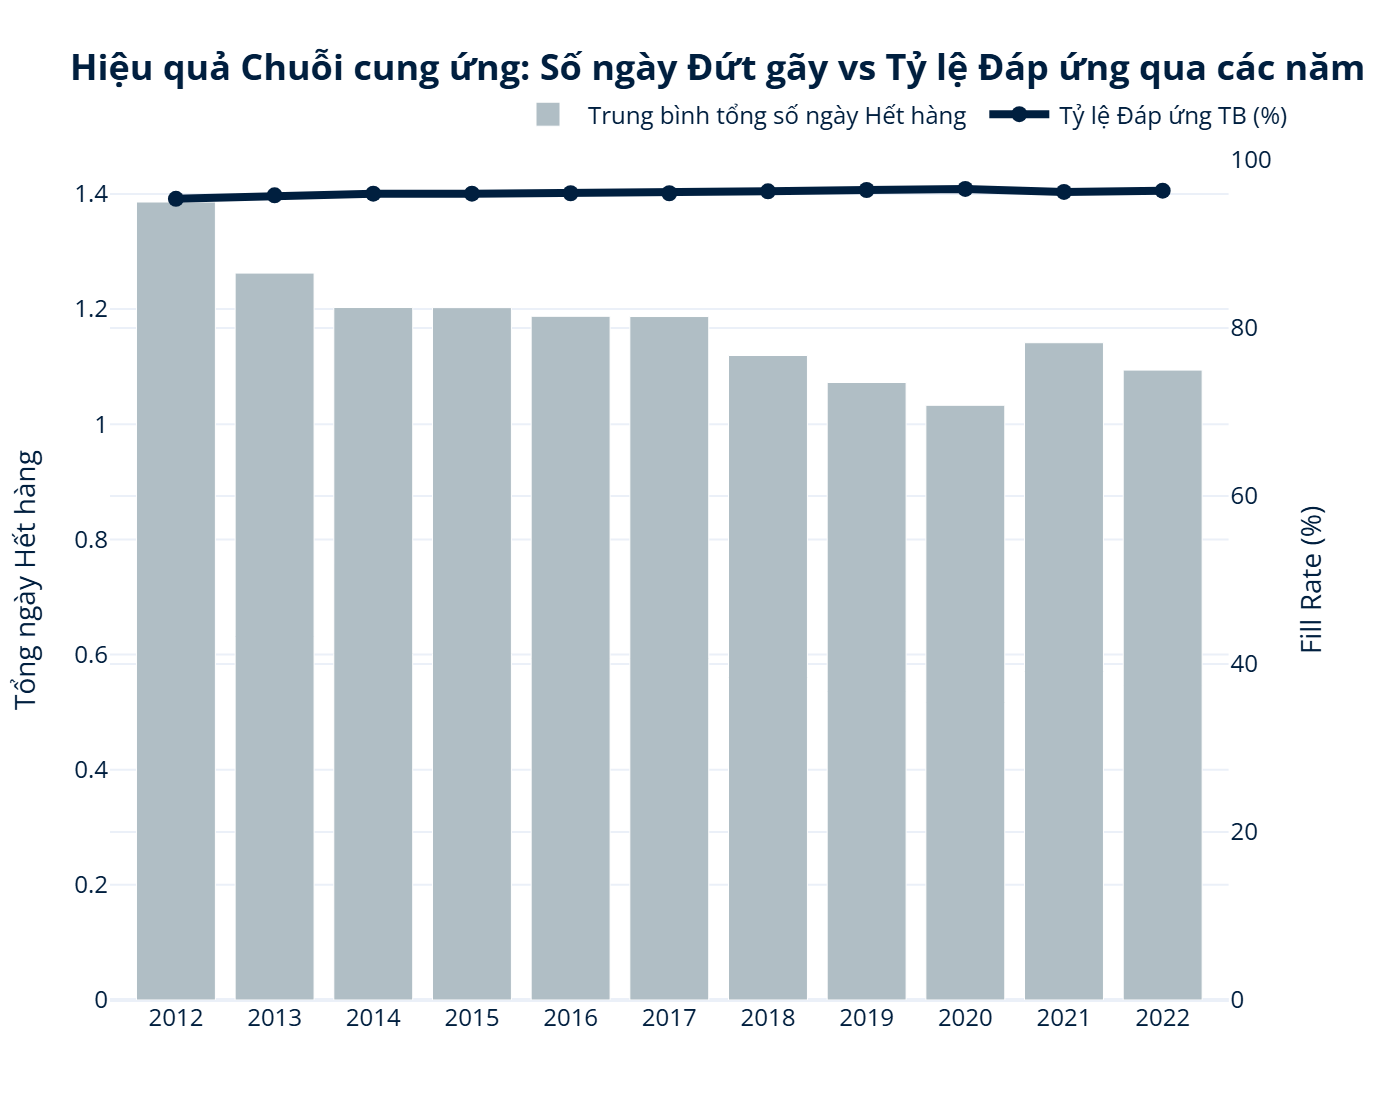
\includegraphics[width=0.8\textwidth]{figures/Hình 2.22.png}
    \caption{Hình 2.22}
    \label{fig:2.22}
\end{figure}

\begin{figure}[H]
    \centering
    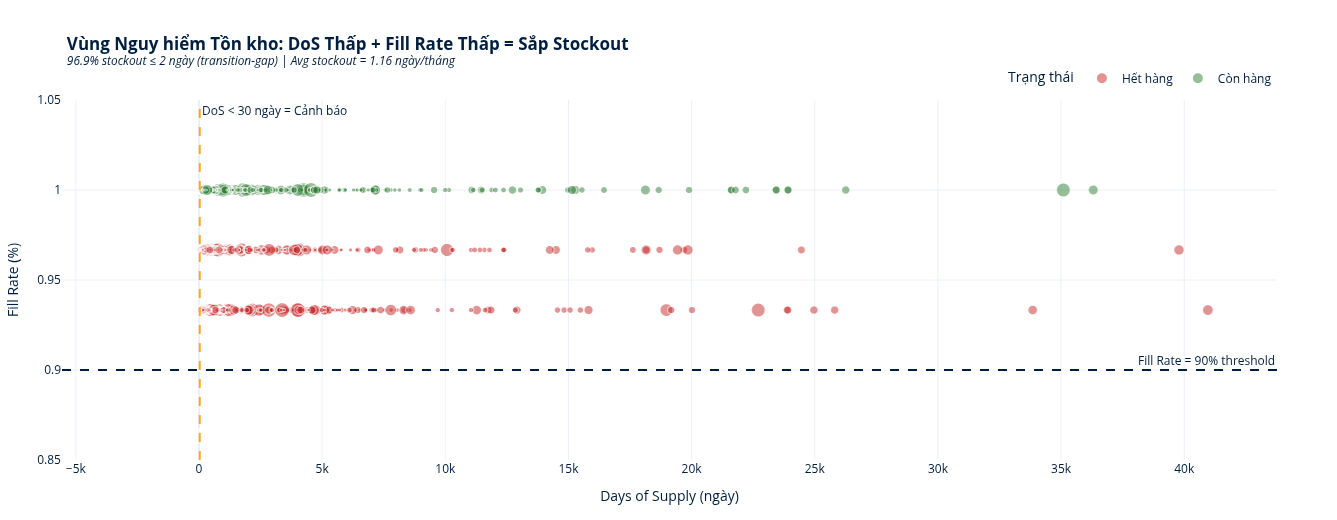
\includegraphics[width=0.8\textwidth]{figures/Hình 2.23.png}
    \caption{Hình 2.23}
    \label{fig:2.23}
\end{figure}

\begin{figure}[H]
    \centering
    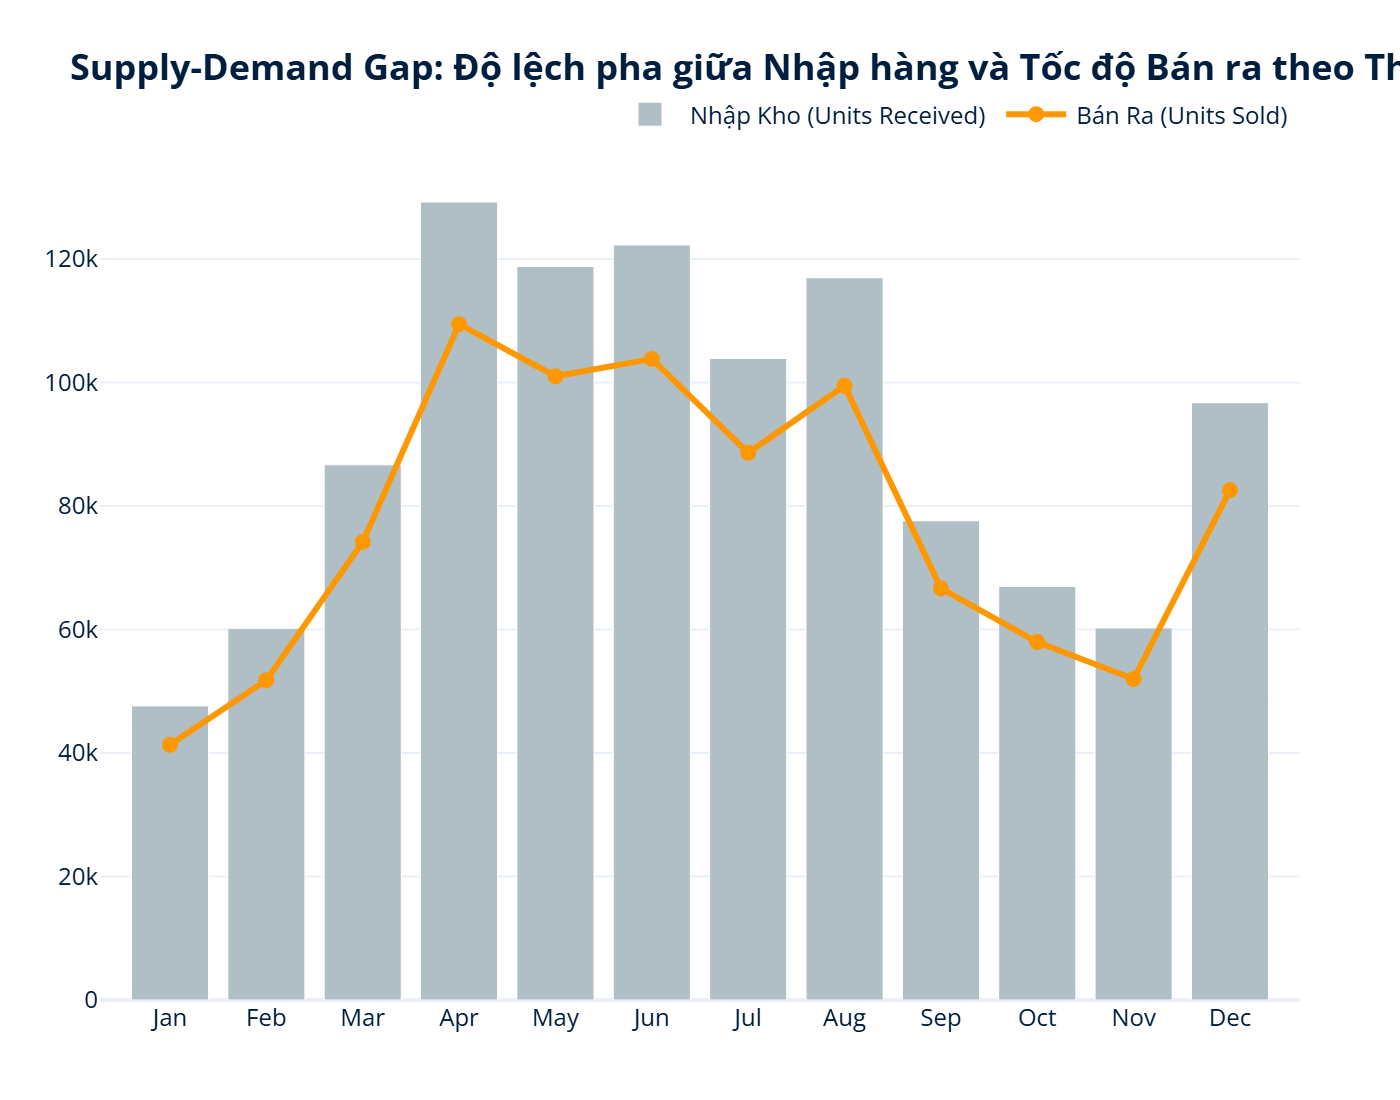
\includegraphics[width=0.8\textwidth]{figures/Hình 2.24.png}
    \caption{Hình 2.24}
    \label{fig:2.24}
\end{figure}

\begin{figure}[H]
    \centering
    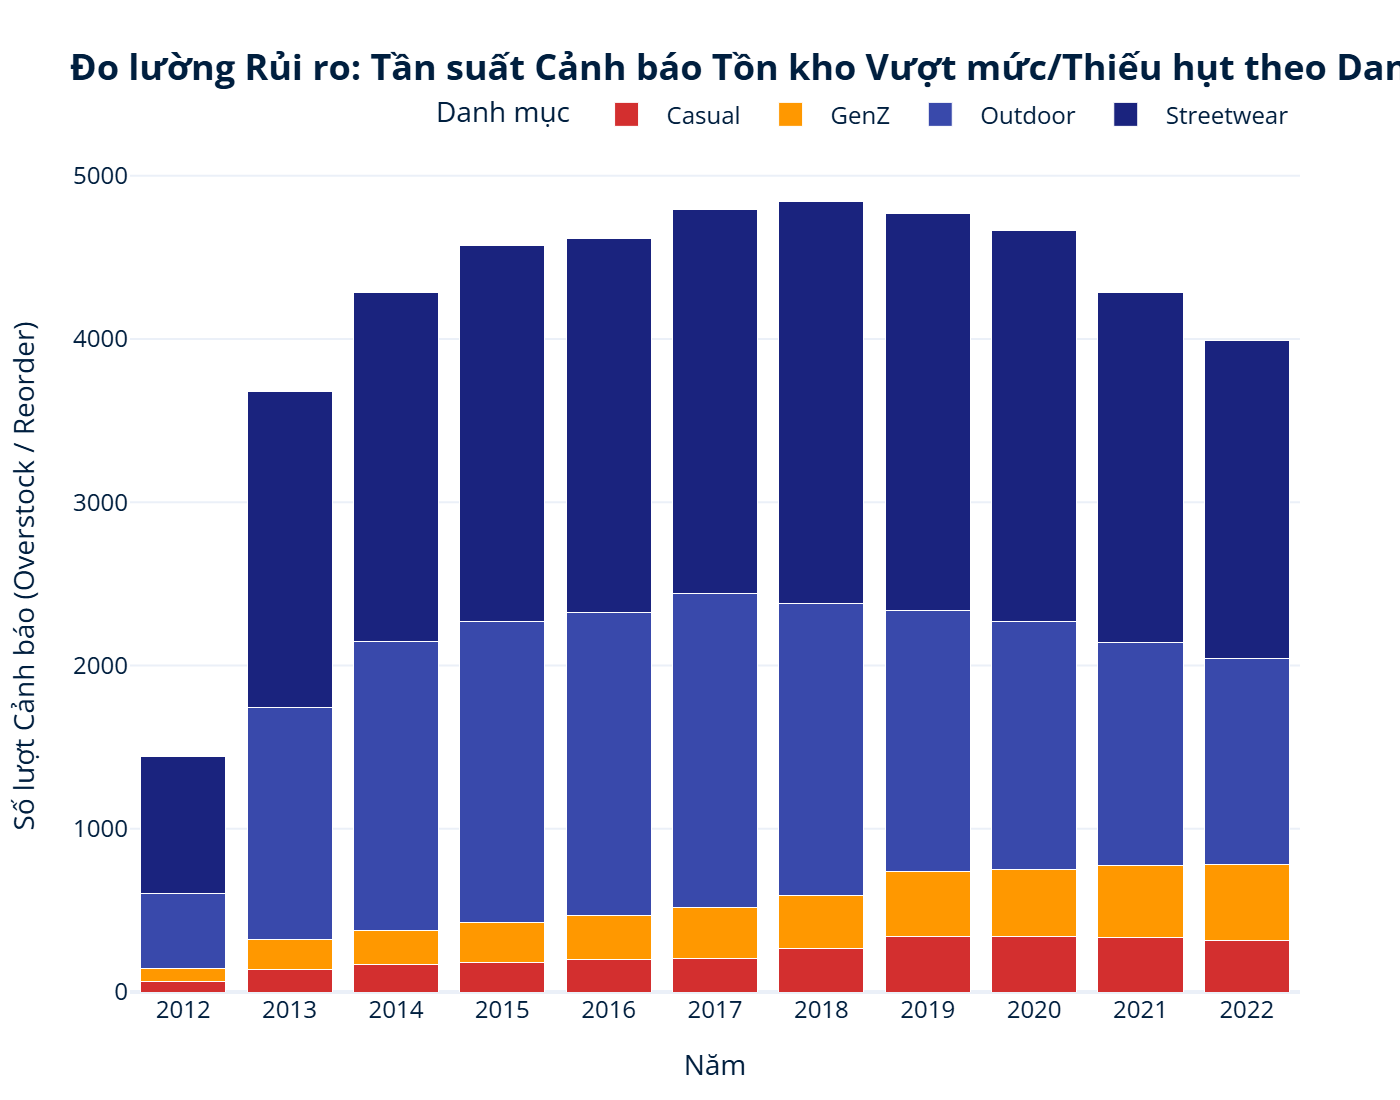
\includegraphics[width=0.8\textwidth]{figures/Hình 2.25.png}
    \caption{Hình 2.25}
    \label{fig:2.25}
\end{figure}

\begin{figure}[H]
    \centering
    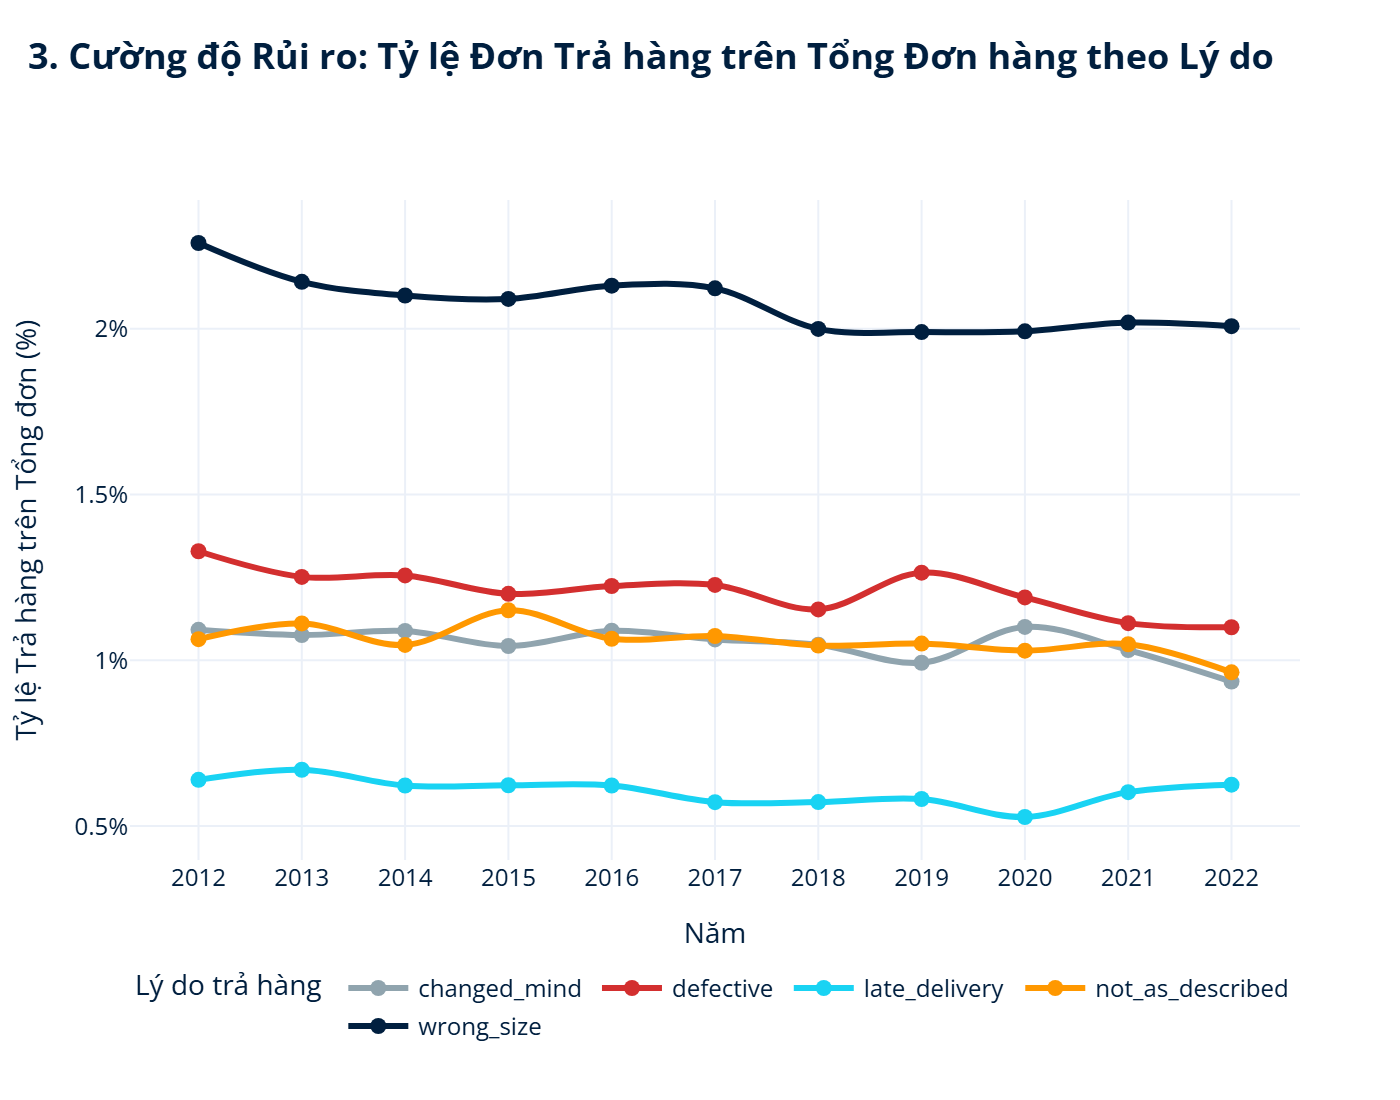
\includegraphics[width=0.8\textwidth]{figures/Hình 2.26.png}
    \caption{Hình 2.26}
    \label{fig:2.26}
\end{figure}

\begin{figure}[H]
    \centering
    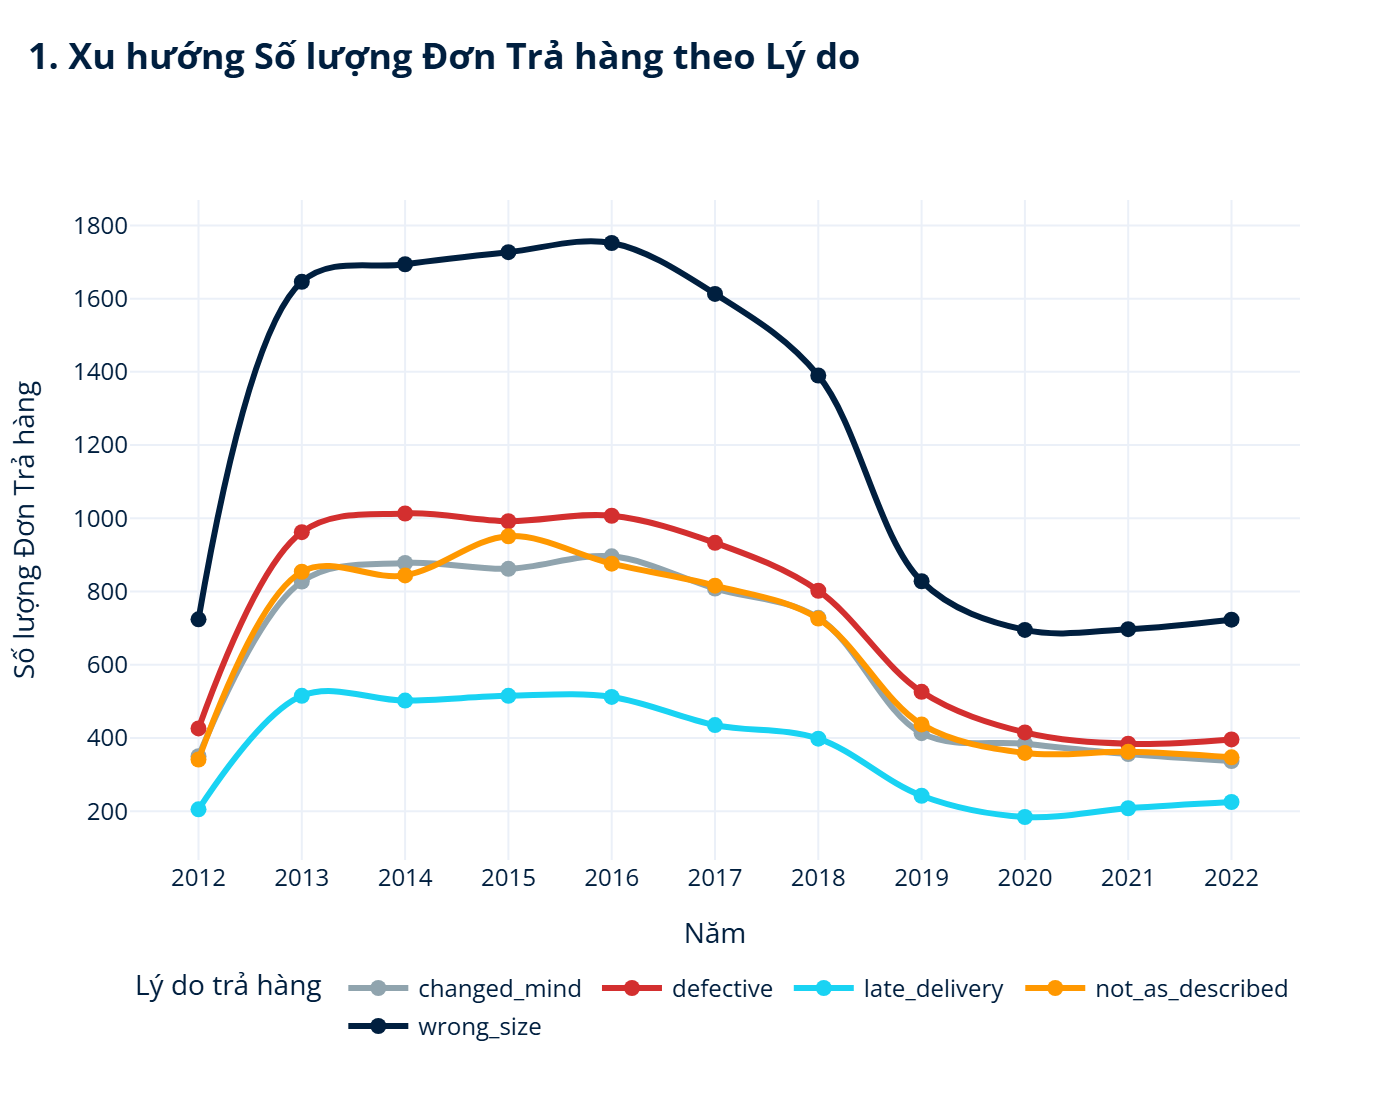
\includegraphics[width=0.8\textwidth]{figures/Hình 2.27.png}
    \caption{Hình 2.27}
    \label{fig:2.27}
\end{figure}

\begin{figure}[H]
    \centering
    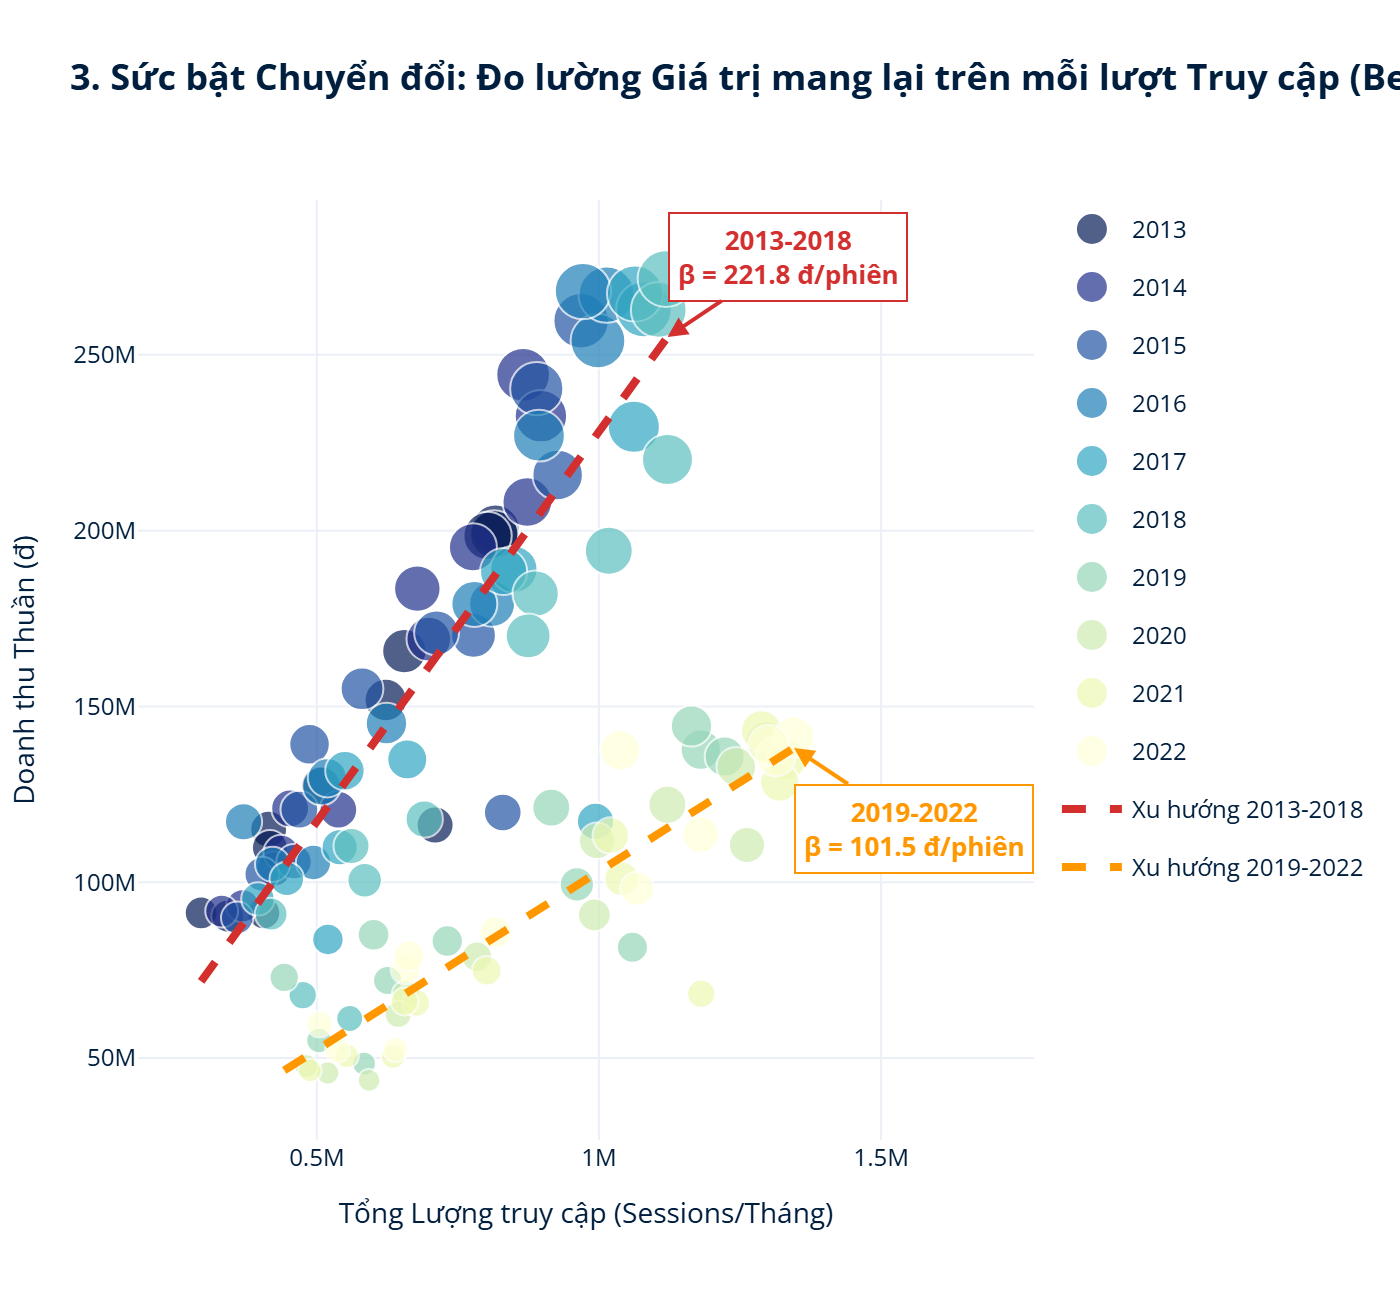
\includegraphics[width=0.8\textwidth]{figures/Hình 2.28.png}
    \caption{Hình 2.28}
    \label{fig:2.28}
\end{figure}

\begin{figure}[H]
    \centering
    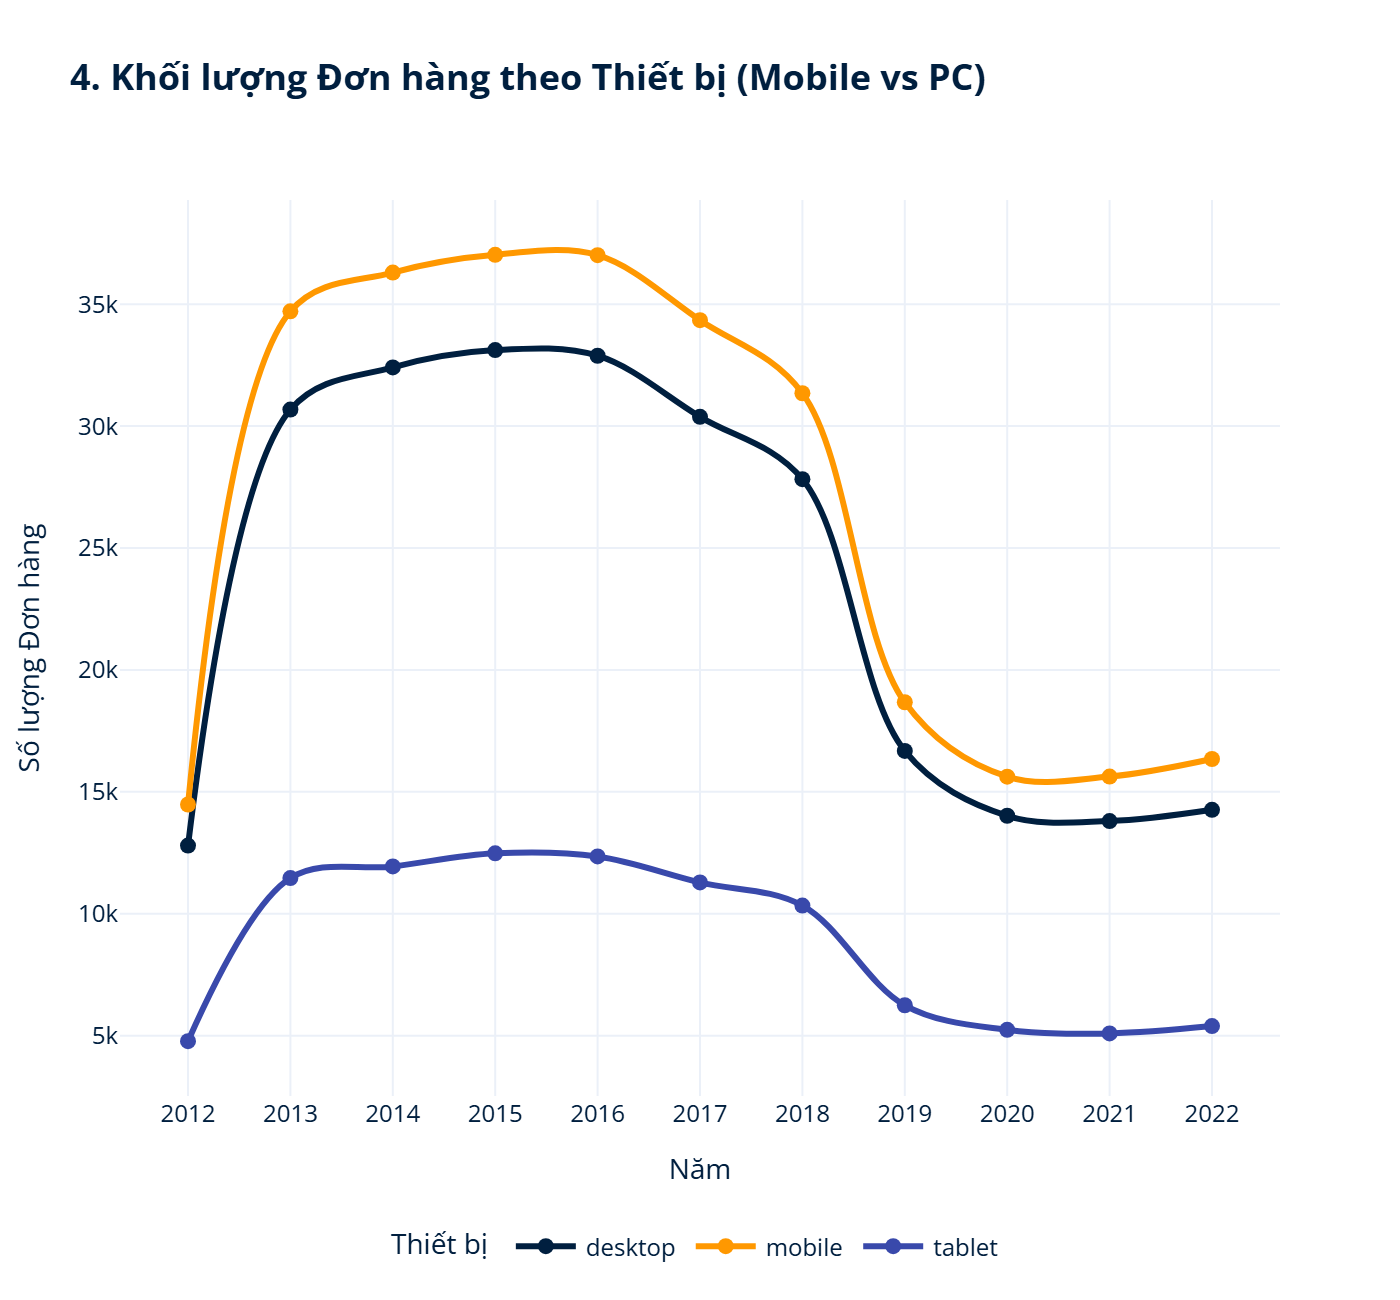
\includegraphics[width=0.8\textwidth]{figures/Hình 2.29.png}
    \caption{Hình 2.29}
    \label{fig:2.29}
\end{figure}

\begin{figure}[H]
    \centering
    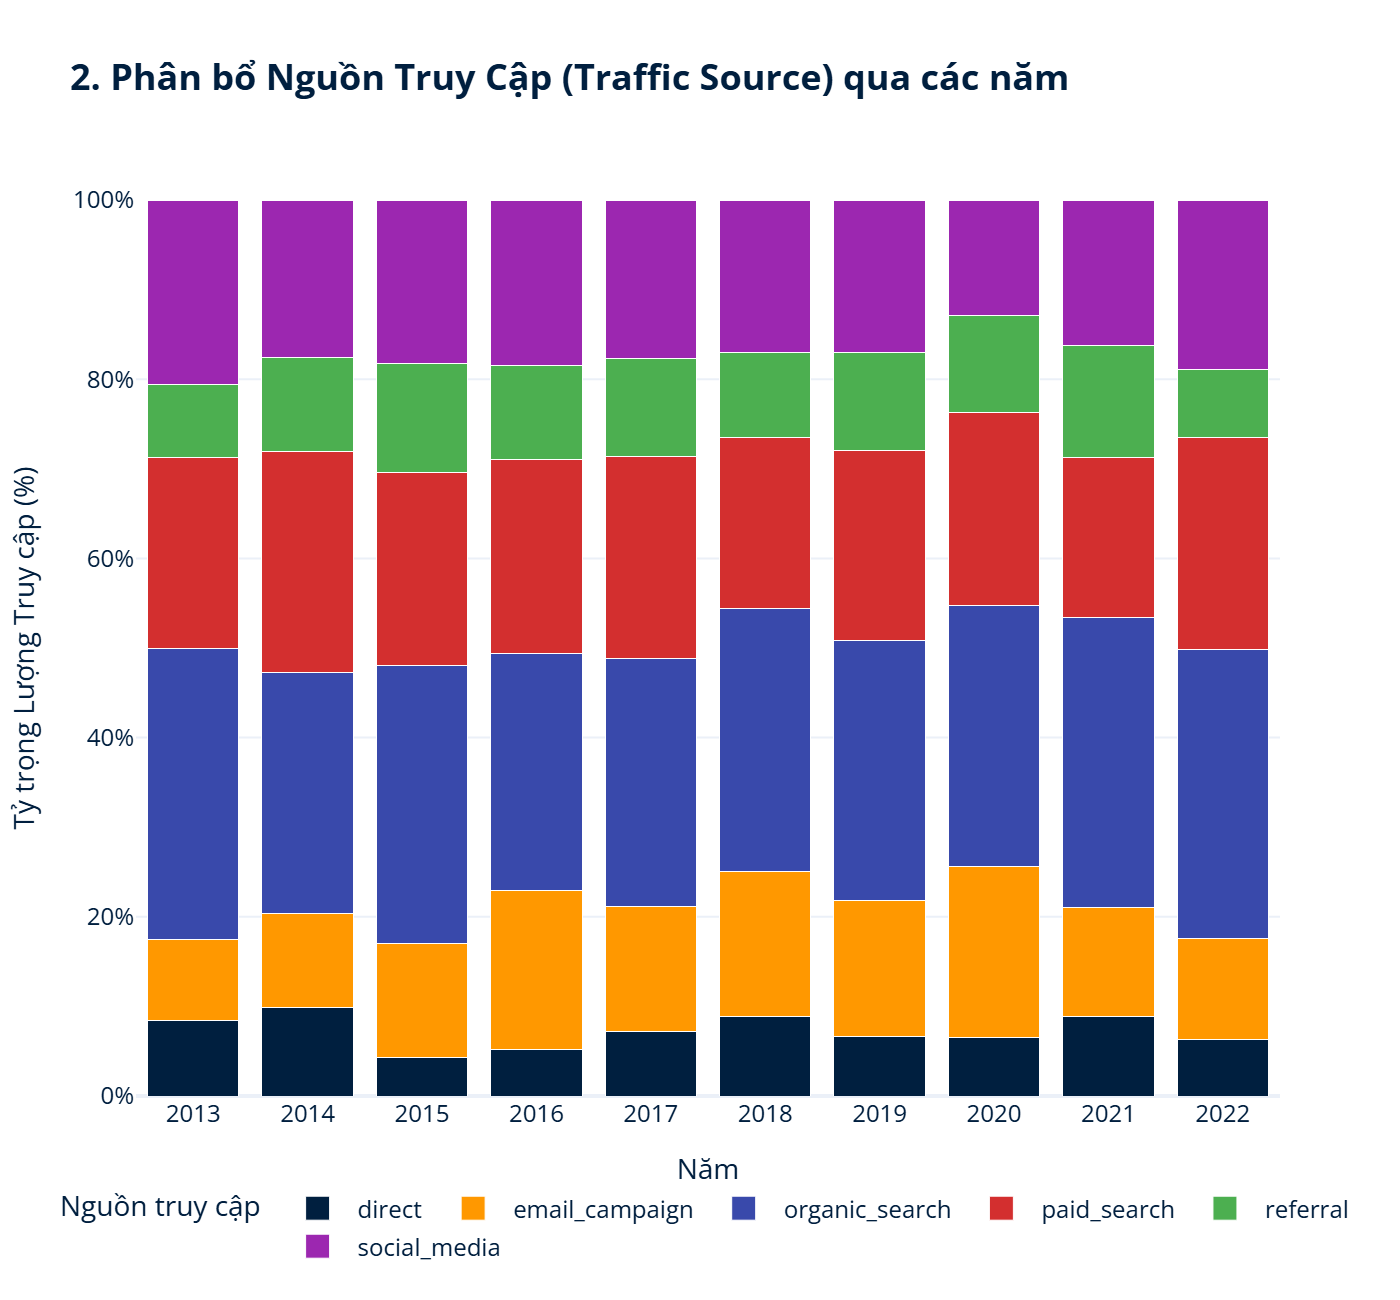
\includegraphics[width=0.8\textwidth]{figures/Hình 2.30.png}
    \caption{Hình 2.30}
    \label{fig:2.30}
\end{figure}

\begin{figure}[H]
    \centering
    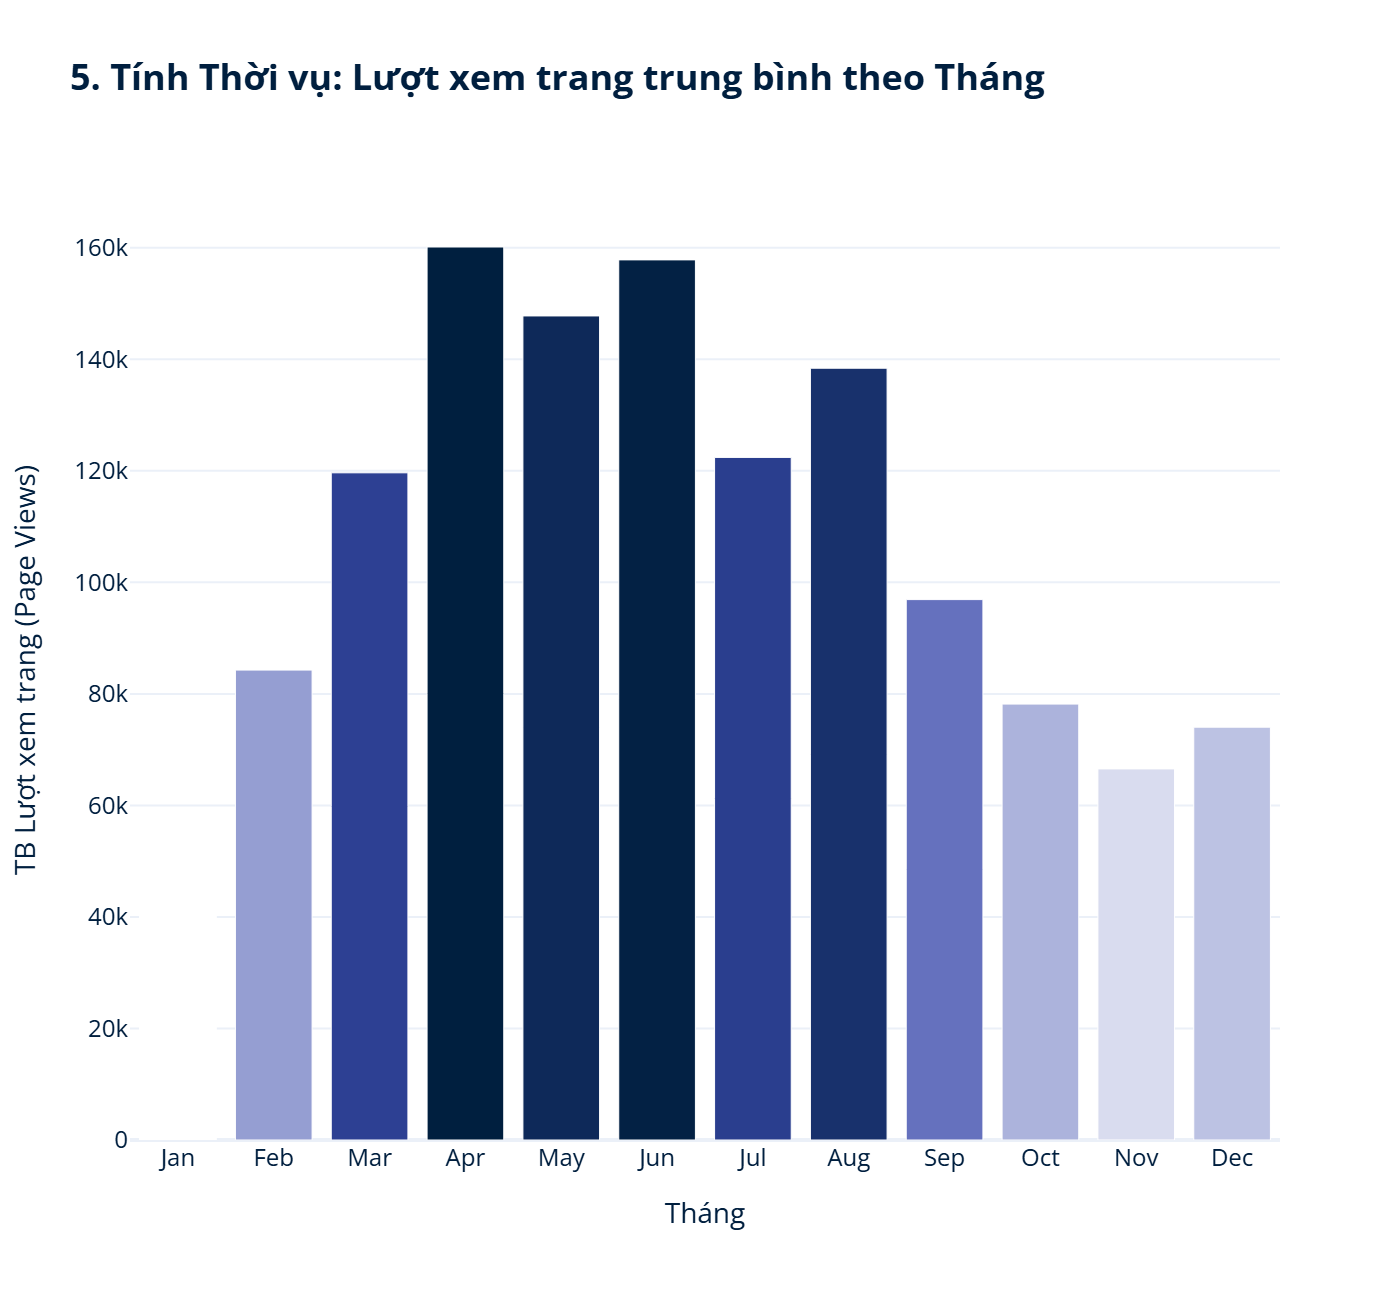
\includegraphics[width=0.8\textwidth]{figures/Hình 2.31.png}
    \caption{Hình 2.31}
    \label{fig:2.31}
\end{figure}

\begin{figure}[H]
    \centering
    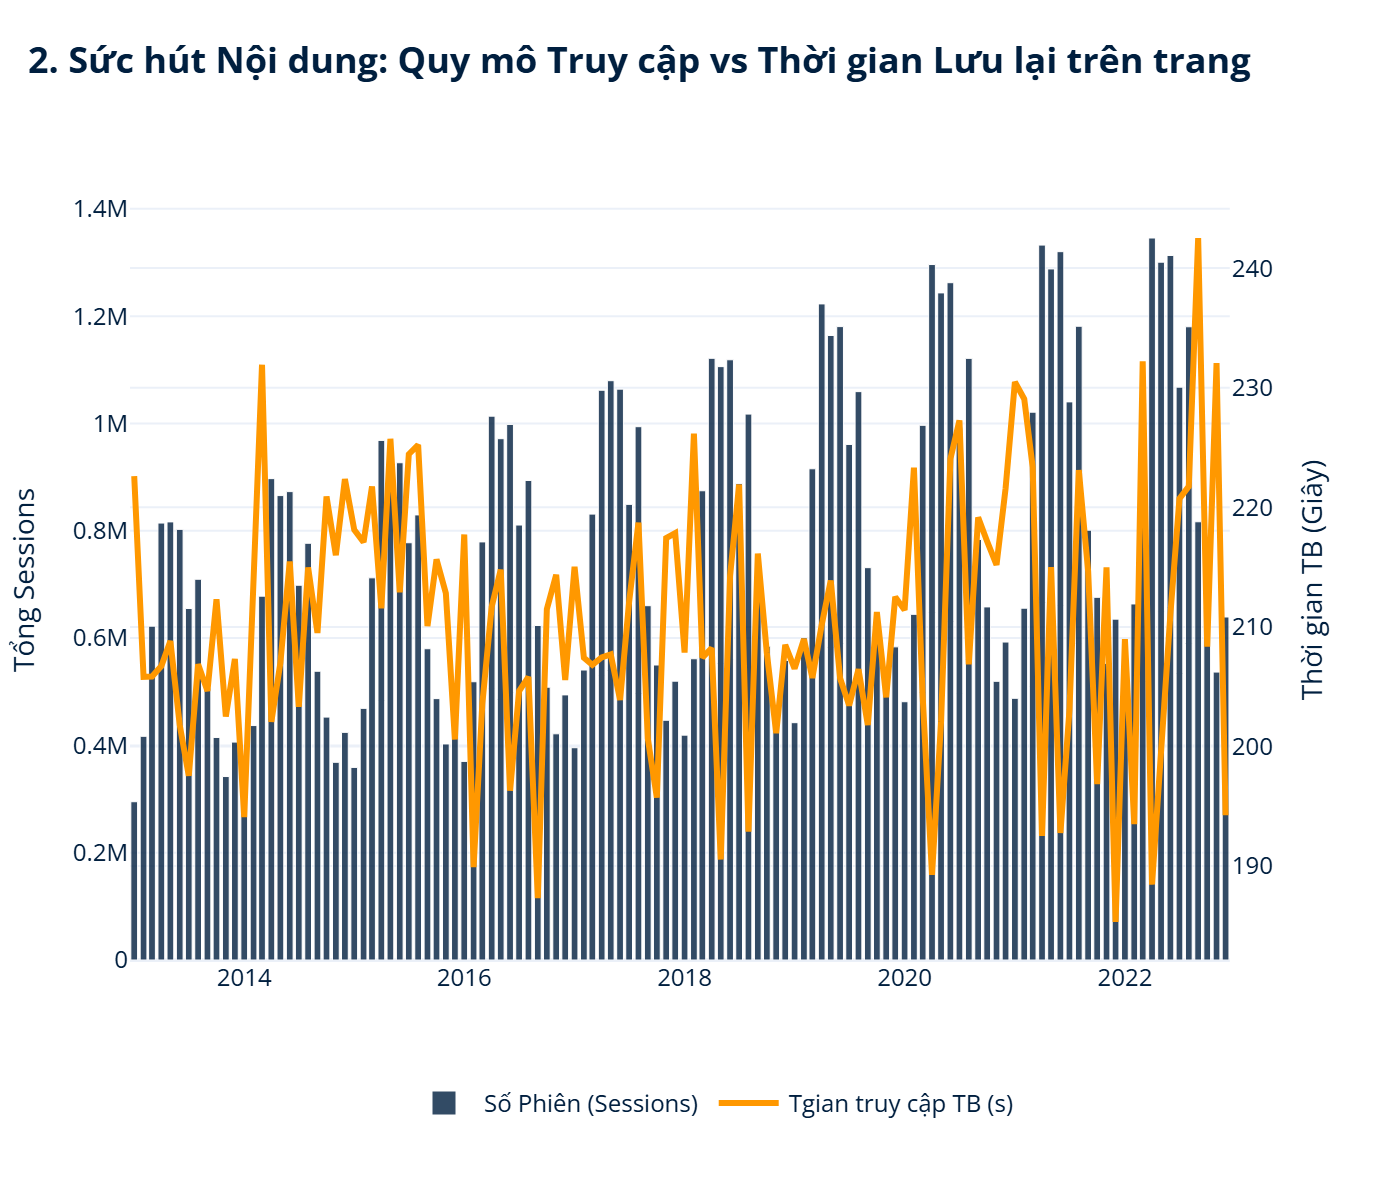
\includegraphics[width=0.8\textwidth]{figures/Hình 2.32.png}
    \caption{Hình 2.32}
    \label{fig:2.32}
\end{figure}

\begin{figure}[H]
    \centering
    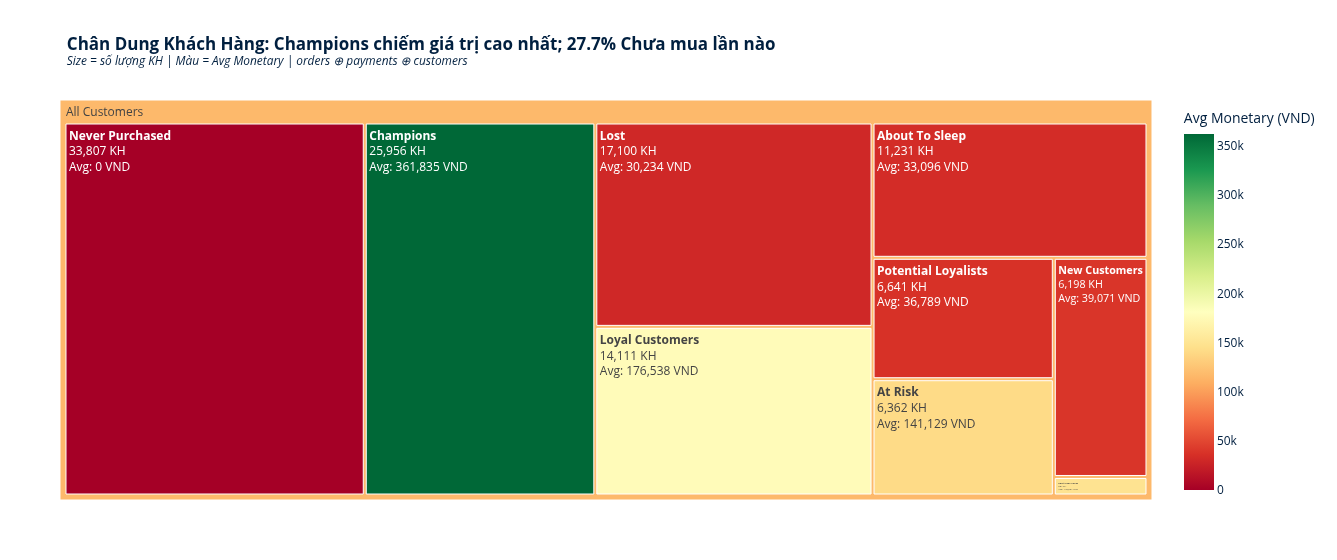
\includegraphics[width=0.8\textwidth]{figures/Hình 2.33a.png}
    \caption{Hình 2.33a}
    \label{fig:2.33a}
\end{figure}

\begin{figure}[H]
    \centering
    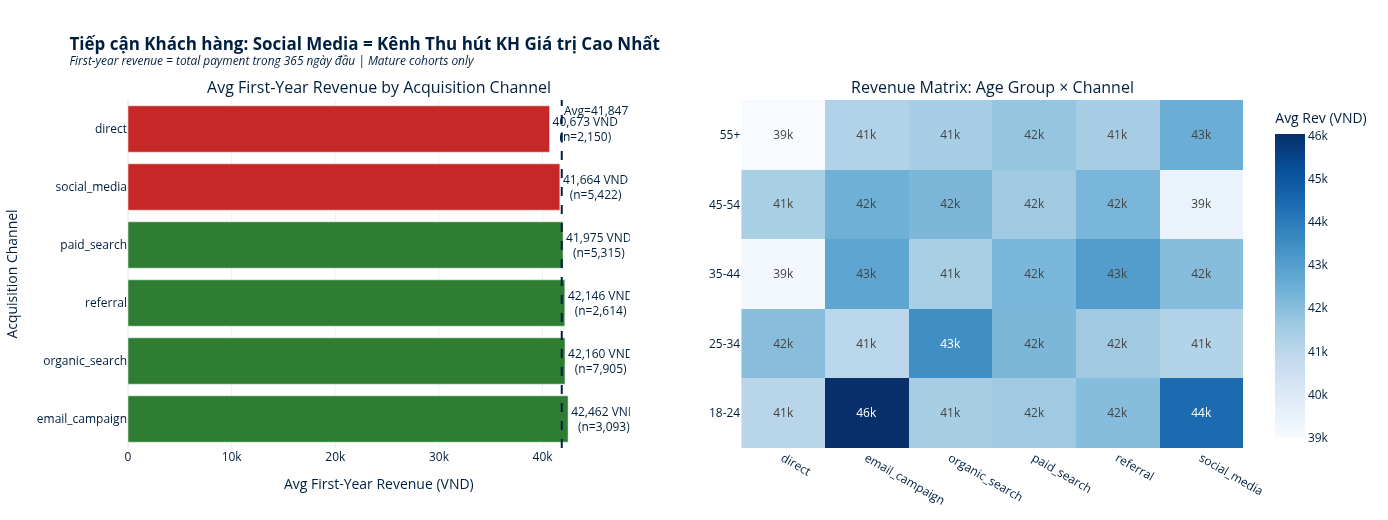
\includegraphics[width=0.8\textwidth]{figures/Hình 2.33b.png}
    \caption{Hình 2.33b}
    \label{fig:2.33b}
\end{figure}

\begin{figure}[H]
    \centering
    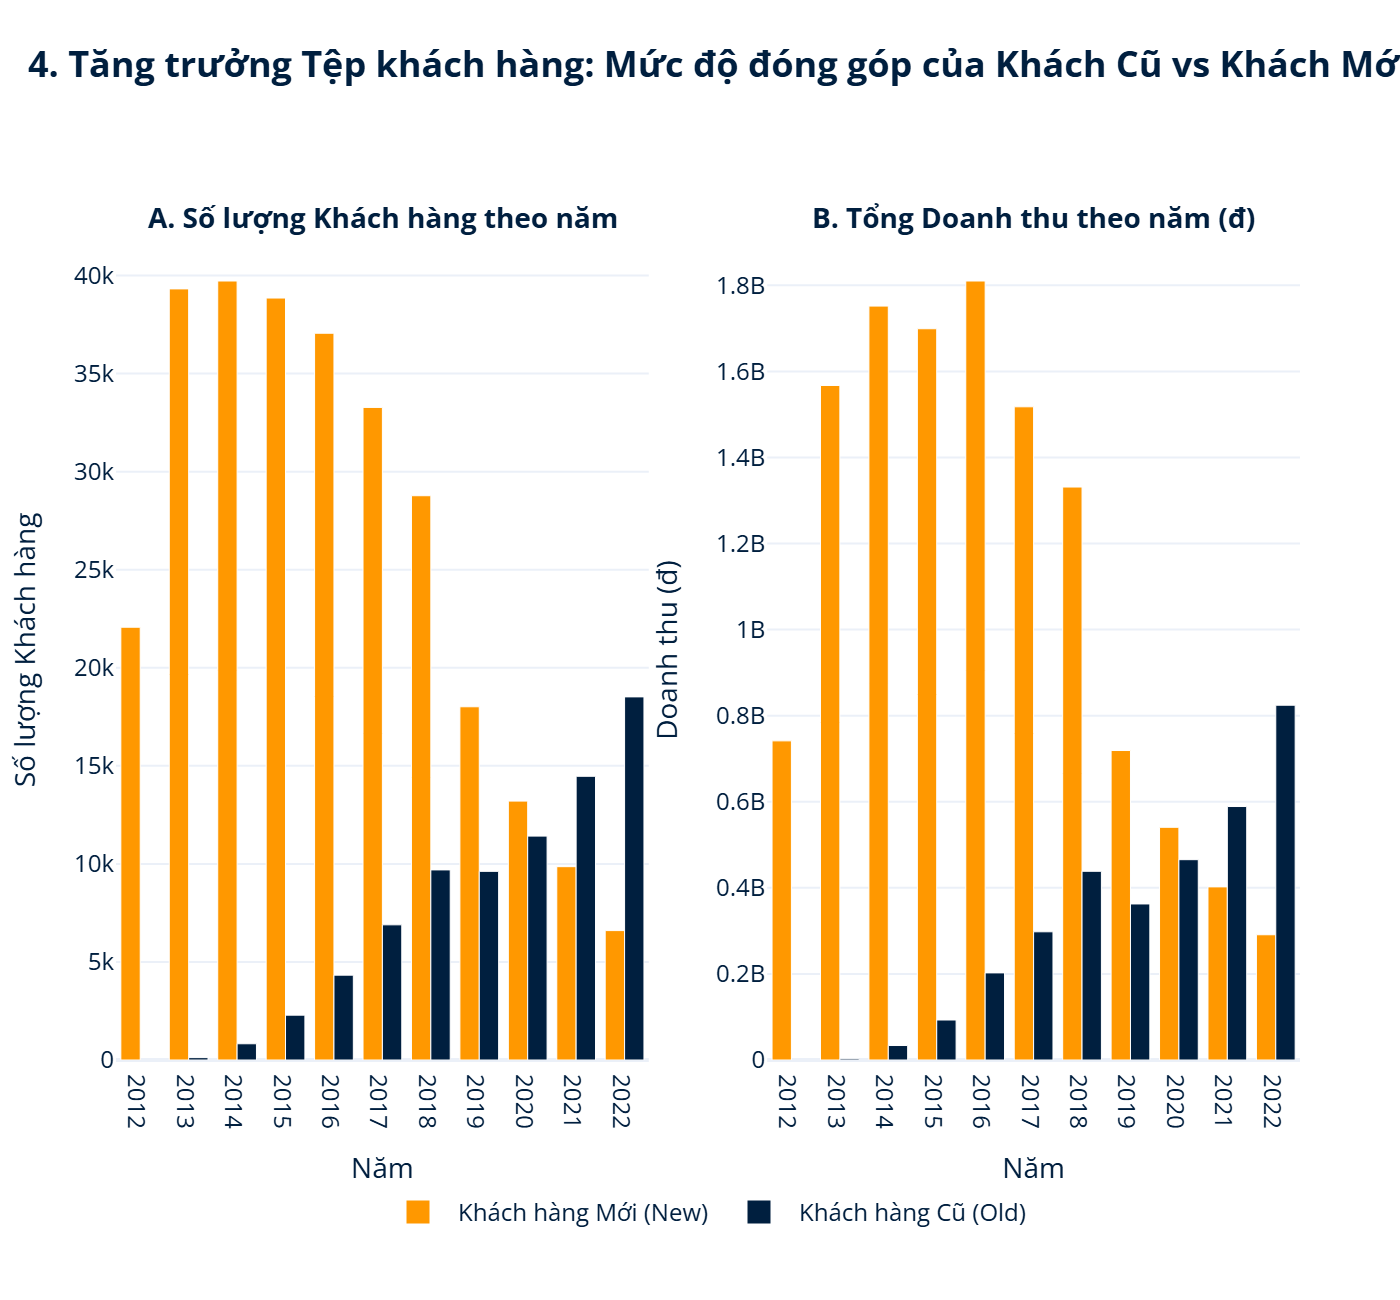
\includegraphics[width=0.8\textwidth]{figures/Hình 2.34.png}
    \caption{Hình 2.34}
    \label{fig:2.34}
\end{figure}

\begin{figure}[H]
    \centering
    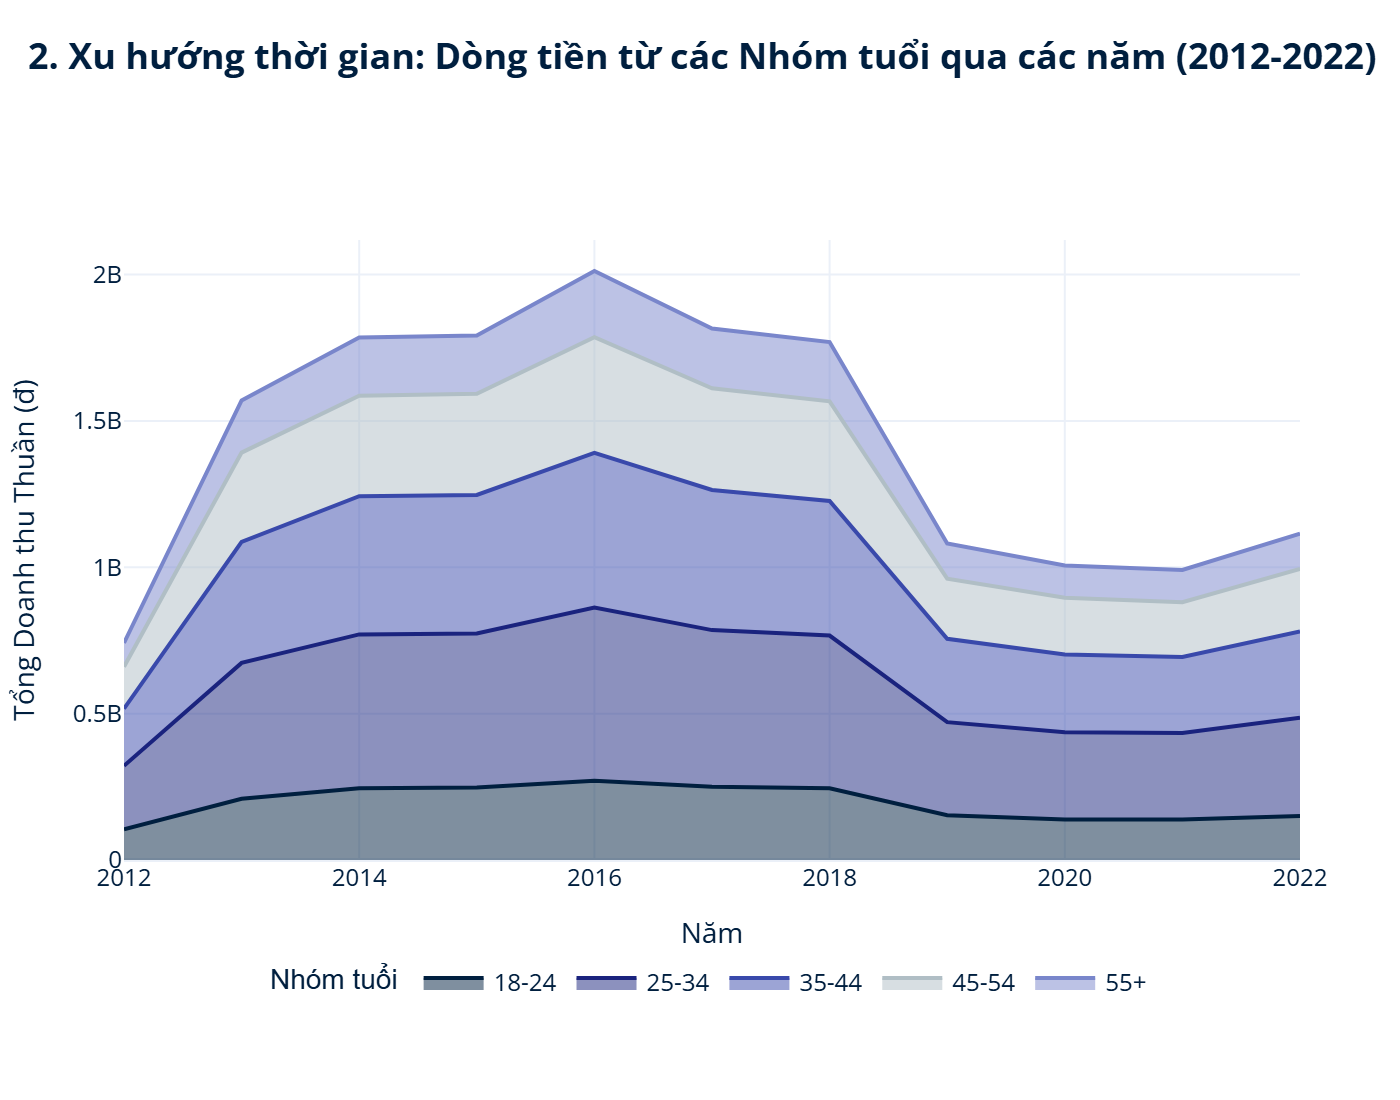
\includegraphics[width=0.8\textwidth]{figures/Hình 2.35.png}
    \caption{Hình 2.35}
    \label{fig:2.35}
\end{figure}

\subsection{Chi tiết khả năng giải thích của mô hình}
\label{app:explainability}

Hình~\ref{fig:shap} và Hình~\ref{fig:gain} trình bày xếp hạng đặc trưng theo hai phương pháp tiếp cận khác nhau. Cả hai phương pháp đều xác nhận vai trò chủ đạo của \texttt{Revenue\_lag\_1} và \texttt{COGS\_lag\_1}.

\begin{figure}[H]
    \centering
    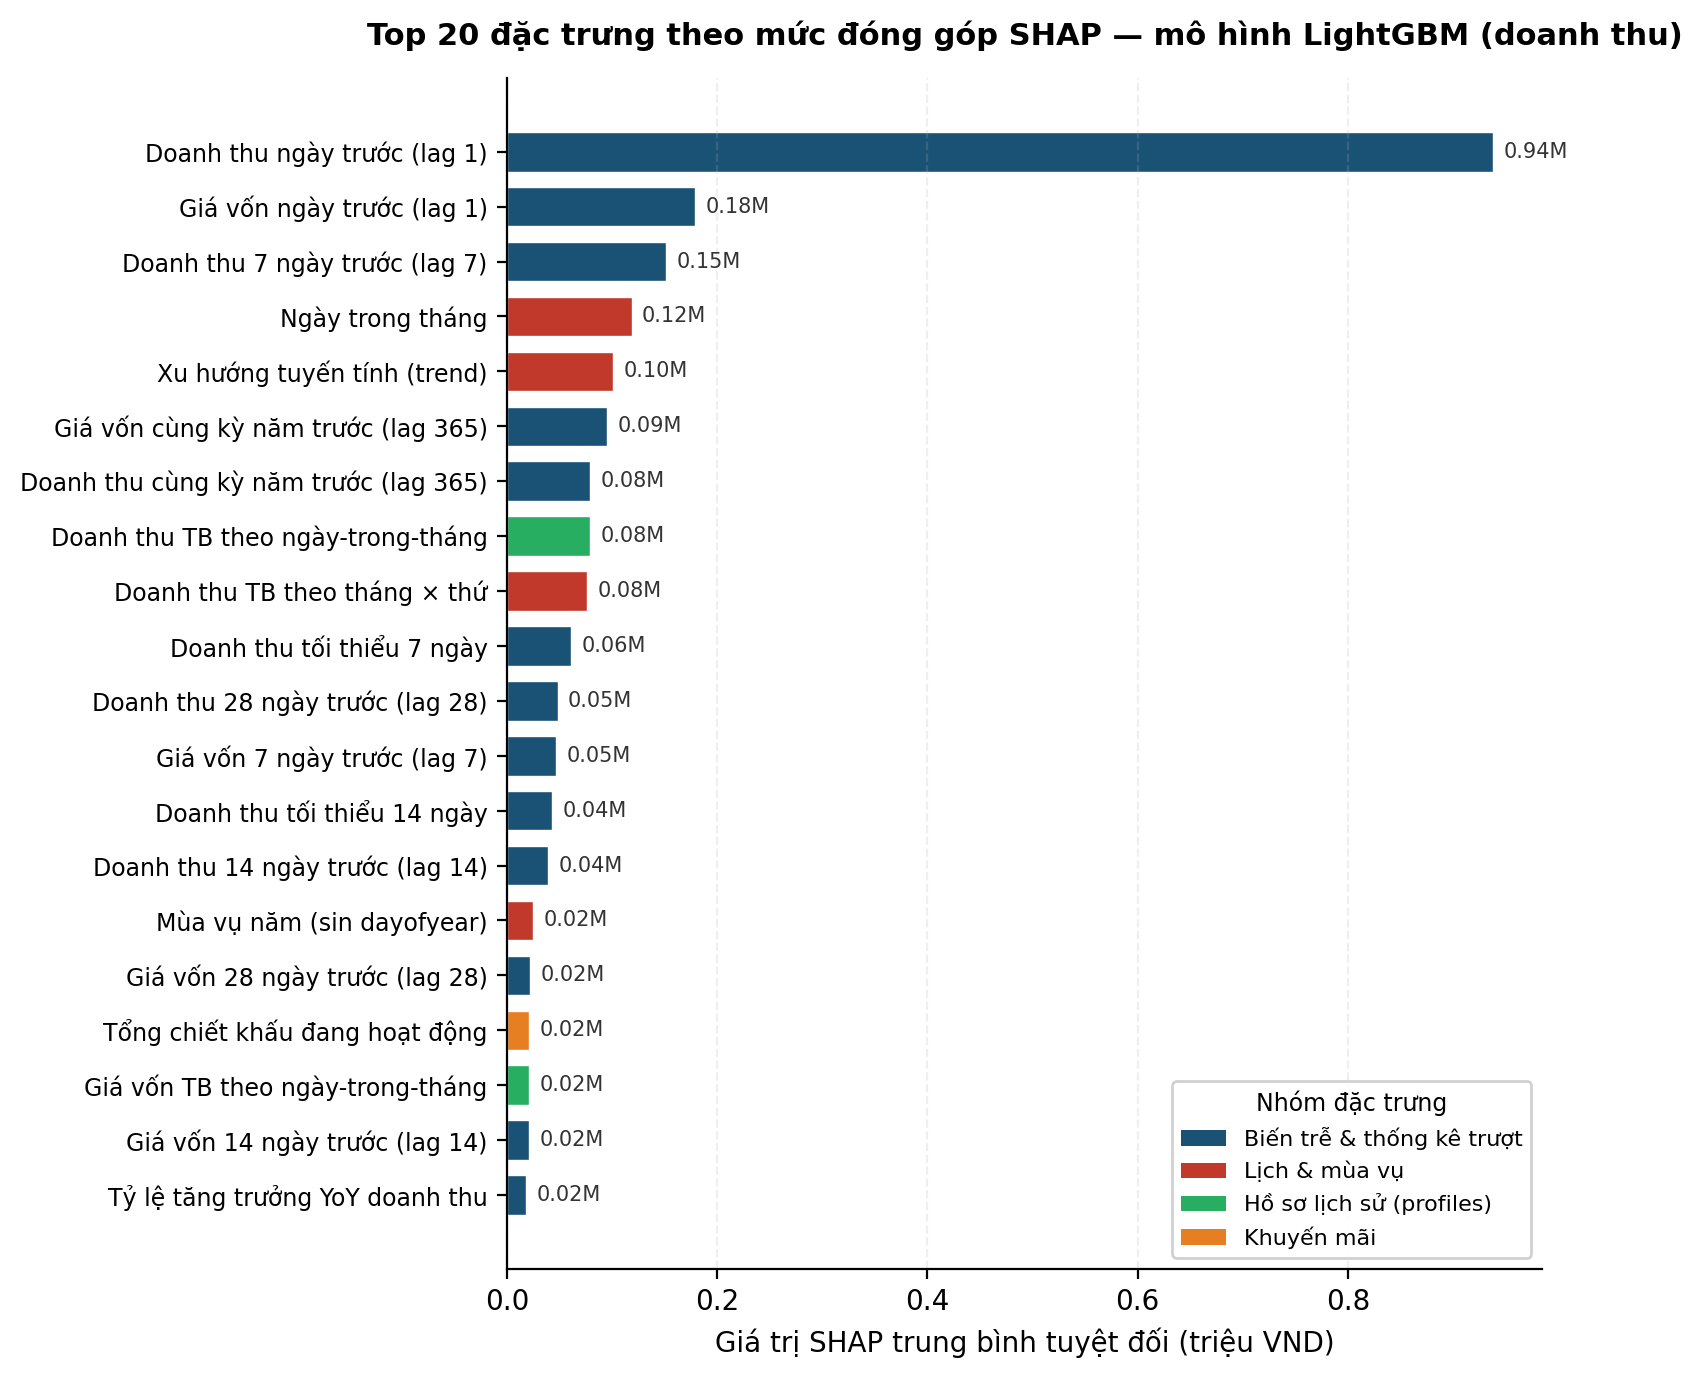
\includegraphics[width=0.82\textwidth]{figures/shap_feature_importance.png}
    \vspace{-0.5em}
    \caption{Top 20 đặc trưng theo giá trị SHAP trung bình tuyệt đối ($\text{mean}\,|\phi_j|$). Màu sắc phân loại: biến trễ \& thống kê trượt (xanh đậm), lịch \& mùa vụ (đỏ), hồ sơ lịch sử (xanh lá), khuyến mãi (cam).}
    \label{fig:shap}
\end{figure}

\begin{figure}[H]
    \centering
    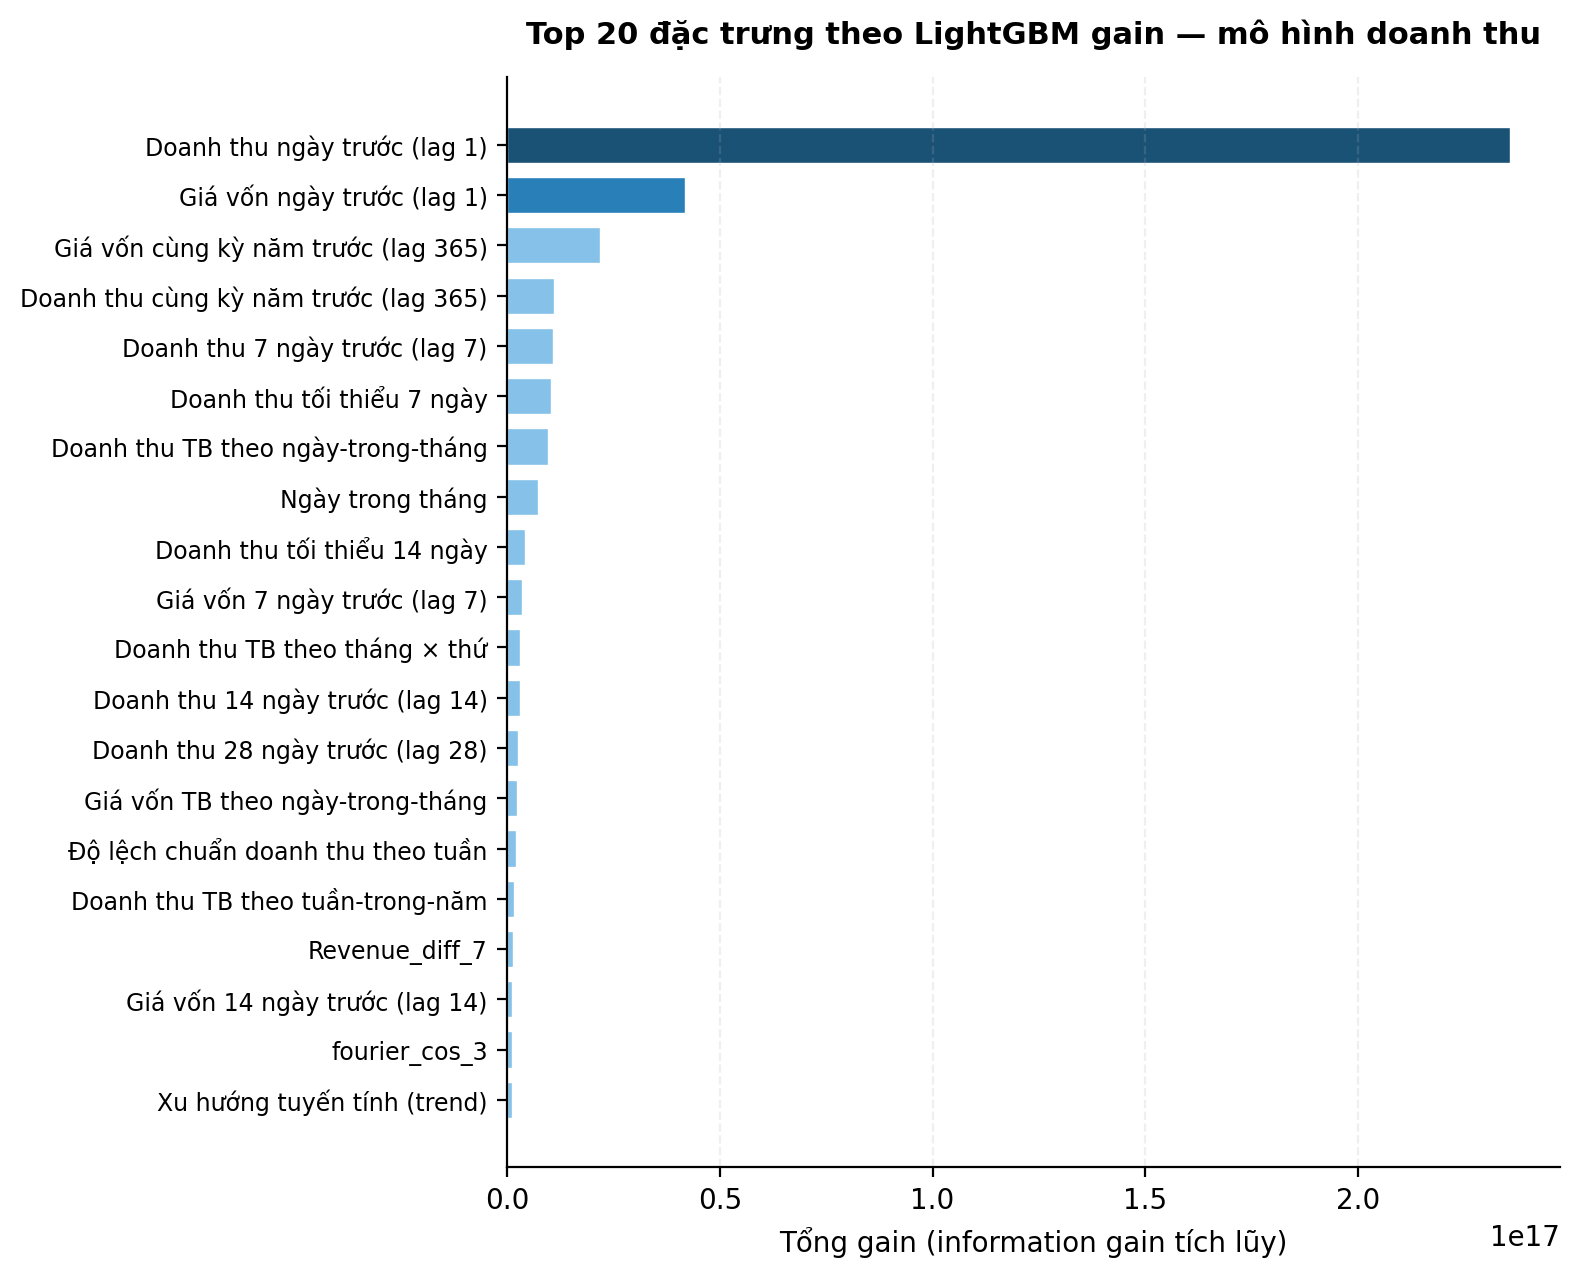
\includegraphics[width=0.78\textwidth]{figures/lgbm_gain_importance.png}
    \vspace{-0.5em}
    \caption{Top 20 đặc trưng theo tổng information gain tích lũy từ cấu trúc cây LightGBM. Cường độ màu tỷ lệ với mức đóng góp tương đối so với đặc trưng hàng đầu.}
    \label{fig:gain}
\end{figure}

Biểu đồ beeswarm (Hình~\ref{fig:beeswarm}) mở rộng phân tích từ giá trị trung bình sang phân phối đầy đủ của các giá trị SHAP, phản ánh phân phối tác động theo chiều giá trị đặc trưng. Hình~\ref{fig:dependence} trình bày biểu đồ phụ thuộc SHAP cho bốn đặc trưng có đóng góp cao nhất, giúp làm rõ hàm quan hệ mà mô hình đã học giữa giá trị đặc trưng và tác động lên dự báo.

\begin{figure}[H]
    \centering
    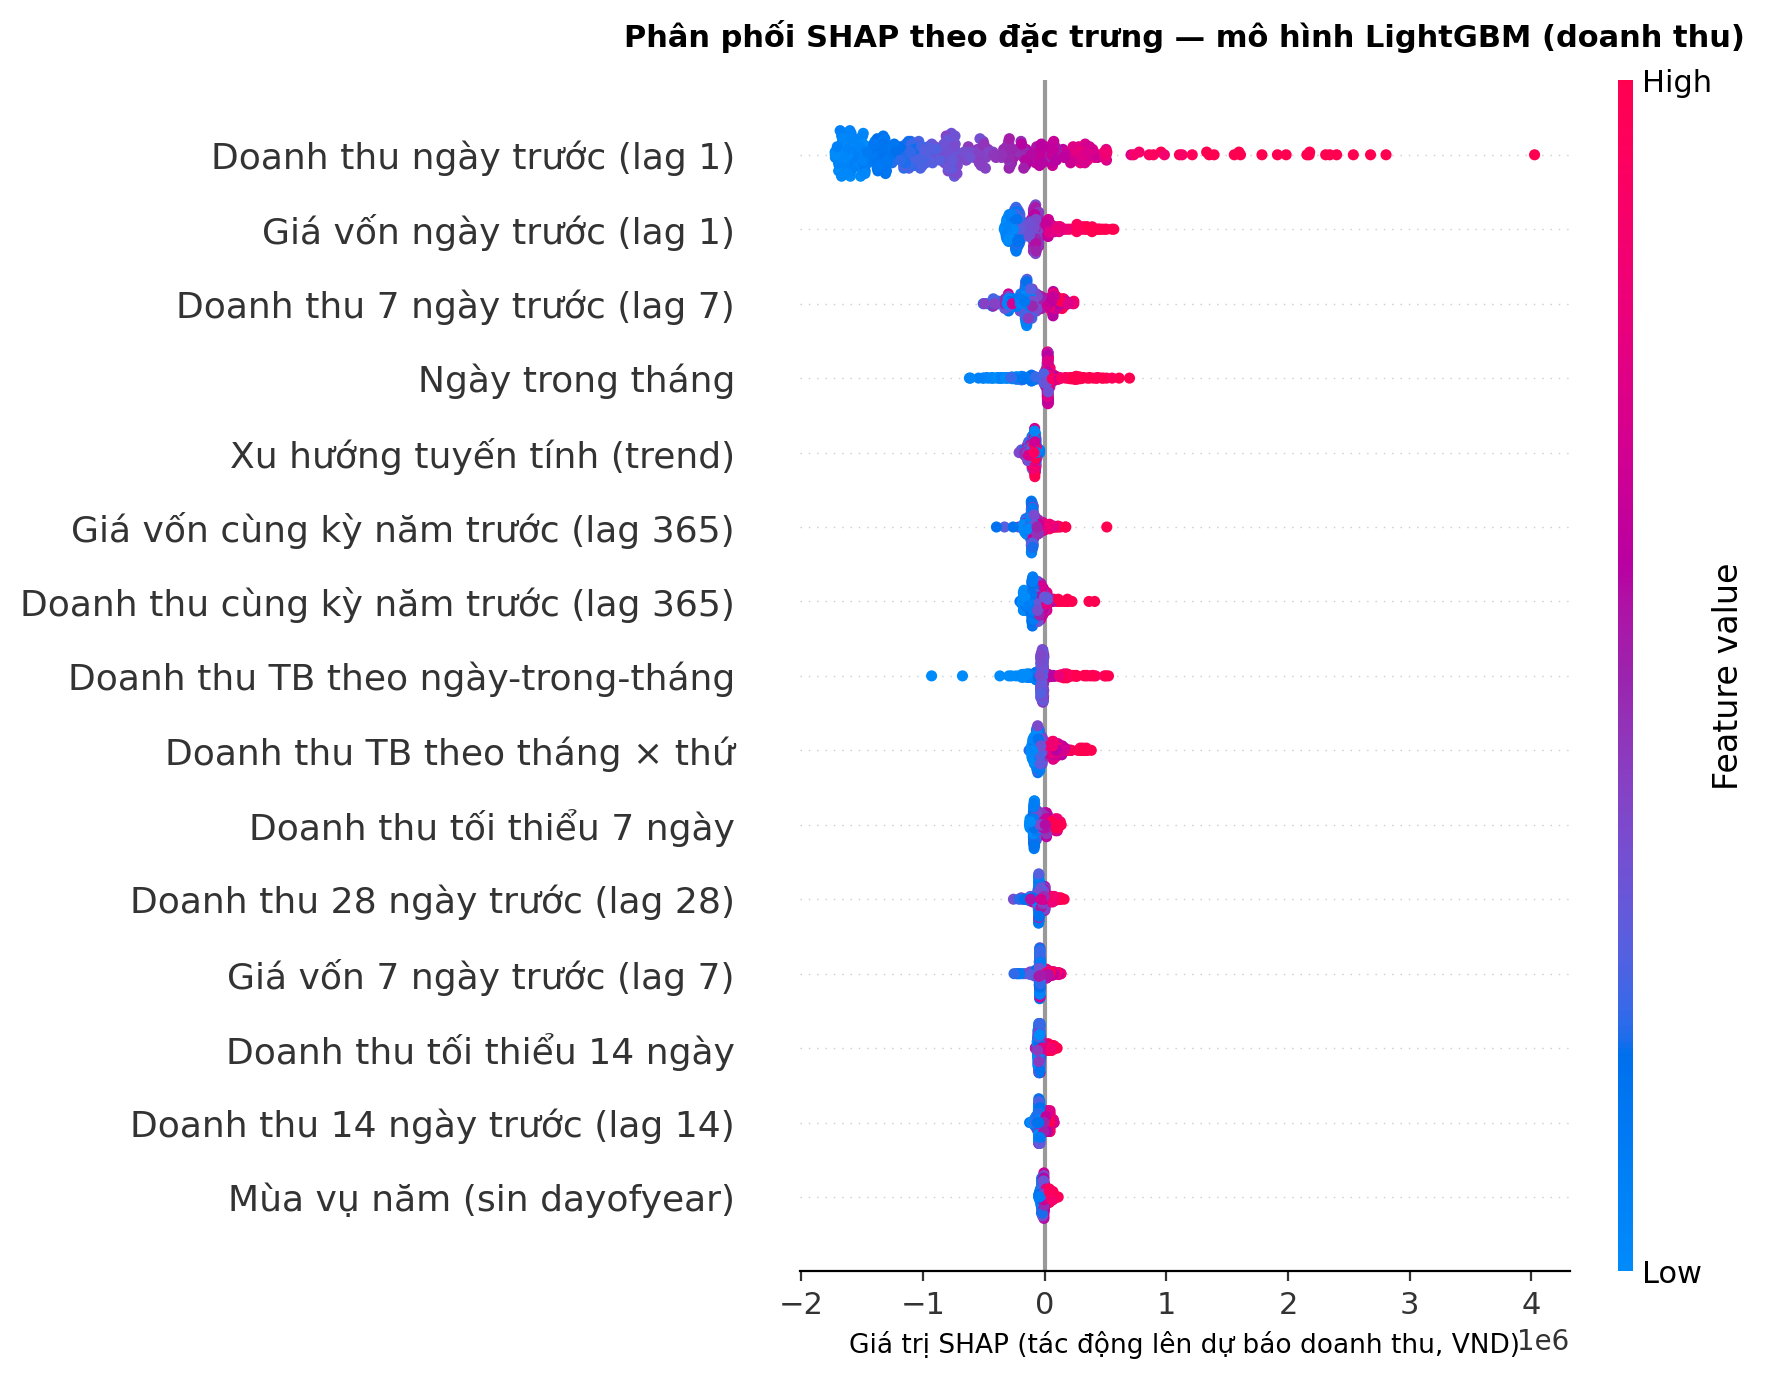
\includegraphics[width=0.82\textwidth]{figures/shap_beeswarm.png}
    \vspace{-0.5em}
    \caption{Biểu đồ beeswarm SHAP cho 15 đặc trưng hàng đầu. Mỗi điểm là một mẫu quan sát; trục hoành là giá trị SHAP (VND); màu sắc mã hóa giá trị gốc của đặc trưng (đỏ = cao, xanh = thấp).}
    \label{fig:beeswarm}
\end{figure}

\begin{figure}[H]
    \centering
    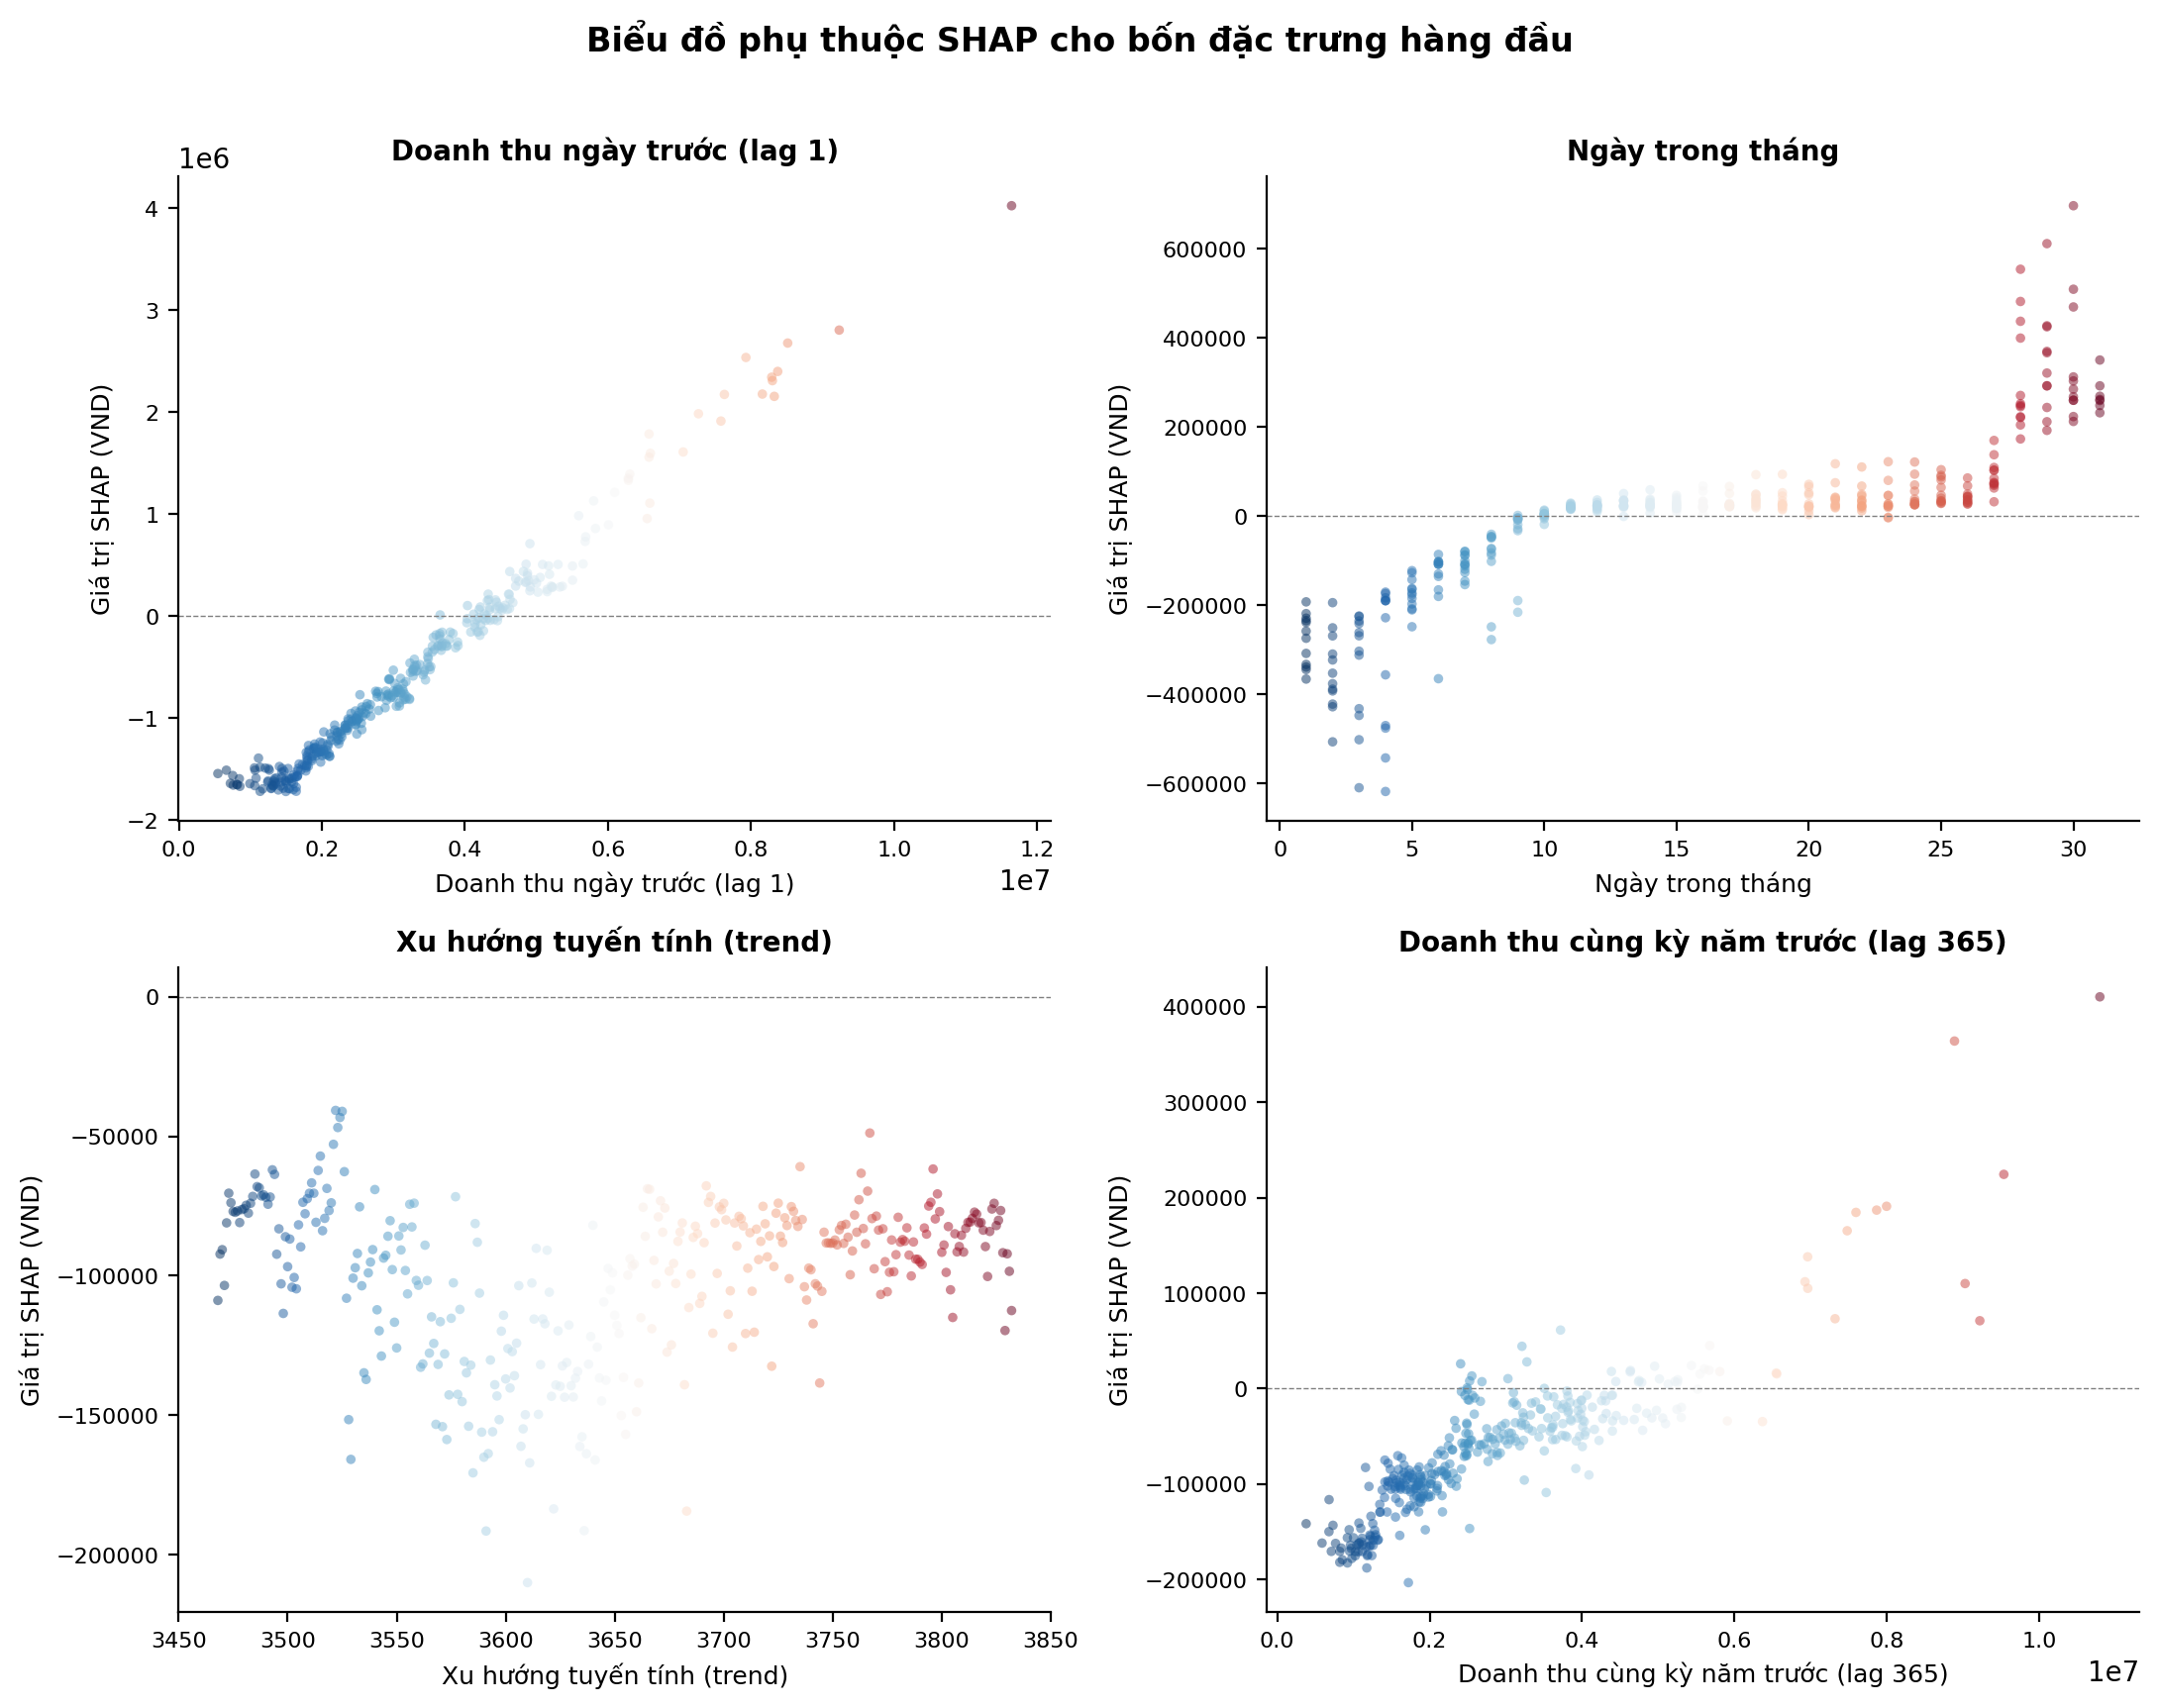
\includegraphics[width=0.7\textwidth]{figures/shap_dependence_top4.png}
    \vspace{-0.5em}
    \caption{Biểu đồ phụ thuộc SHAP cho bốn đặc trưng hàng đầu. Trục hoành: giá trị gốc của đặc trưng; trục tung: giá trị SHAP (VND); màu sắc mã hóa giá trị đặc trưng. Đường nét đứt đánh dấu mức tác động bằng không.}
    \label{fig:dependence}
\end{figure}

\subsection{Nhật ký cấu hình mô hình thực nghiệm cốt lõi}
\label{app:experiments}

Bảng~\ref{tab:experiments} hệ thống hóa 20 cột mốc nghiên cứu định lượng đóng vai trò định hình lại toàn bộ không gian tham số và phương pháp biểu diễn mô hình trong quá trình phát triển hệ thống học máy.

\begin{table}[H]
\caption{Nhật ký cấu hình các mô hình thực nghiệm cốt lõi (model R\&D tracker)}
\label{tab:experiments}
\centering
\small
\begin{tabular}{@{}llp{7cm}rr@{}}
\toprule
EX & Tên mô hình / cấu trúc & Định nghĩa \& phương pháp cải tiến & CV MAE & LB MAE \\
\midrule
01 & Naive Baseline & Dự báo kỳ vọng qua trung bình mùa vụ quá khứ. & 837,000 & 1,247,026 \\
03 & LightGBM Recursive & Sử dụng tập đặc trưng cơ bản và tự hồi quy. & 560,000 & 973,611 \\
05 & N-HiTS Deep Learning & Kiến trúc mạng nơ-ron dự báo trực tiếp đa bước. & 557,000 & 1,287,946 \\
06 & Weighted Ensemble & Thử nghiệm kết hợp mô hình tuyến tính đơn giản. & - & 861,132 \\
18 & Ensemble-Step Research & Đánh giá hàm lượng thông tin đa mô hình đệ quy. & 570,000 & 859,853 \\
19 & Robust Dual-Weight & Phân phối hàm trọng số hội tụ phi đối xứng. & 599,000 & 834,681 \\
20 & Recency-Weighted & Thiết lập trọng số qua độ tương đồng chu kỳ gần. & 564,000 & 830,584 \\
21 & Deep FE Recency & Bổ sung phân bố cấu trúc hành vi khách hàng mới. & - & 820,000 \\
22 & \textbf{Deep FE Holidays} & \textbf{Tích hợp đặc trưng khoảng cách chu kỳ nghỉ lễ.} & 554,000 & 796,018 \\
24 & \textbf{Deep FE + Double Date} & \textbf{Mô hình đệ quy: tích hợp hiệu ứng sự kiện chuỗi.} & 590,000 & 795,838 \\
25 & Context-Aware FE & Đặc trưng sự kiện nhị phân ngắt quãng (quá khớp). & 617,000 & 842,405 \\
26 & Clean Continuous FE & Lượng hóa nhị phân bằng hàm khoảng cách. & 613,000 & - \\
49 & YoY-Growth Stateless & Cấu trúc phi trạng thái tham chiếu tăng trưởng YoY. & 752,000 & 978,938 \\
50 & Lag-365 Direct Model & Dự báo trực tiếp thông qua biên độ tự hồi quy dài. & 805,000 & - \\
51 & Lag-365 Recursive & Kết hợp Lag-365 và tự hồi quy giữ mức cơ sở. & 769,000 & 917,935 \\
-- & \textit{Bridge Blends (w10)} & Kết hợp lai 90\% đệ quy (EX-24) \& 10\% (EX-51). & - & $\approx$792,300 \\
-- & \textbf{EX-51 Bridge w15} & \textbf{Kiến trúc lai: 85\% đệ quy + 15\% phi trạng thái.} & - & \textbf{791,764} \\
52 & Monthly Recalibration & Tái chuẩn hóa phân phối dư lượng hàng tháng. & \textbf{726,000} & 923,416 \\
52 & Recalib Bridge w15/w30 & Kiểm thử lai có tái hiệu chuẩn dư lượng hàng tháng. & - & $>$798,000 \\
\bottomrule
\end{tabular}
\end{table}

\end{document}